\chapter{Results}
\label{chap:results}

This works goals were divided in basically three steps, configuration, transmission
and reception, having these three steps barely working it is possible to make a
transmission and analyze data. It is possible to see in figure \ref{fig:setup}
how the hardware is arranged and in figure \ref{fig:setupbd} it is possible to
behold the setup's block diagram, which gives the idea of the complexity behind
the design and how each component is connected.

%foto setup pronto
\begin{figure}[htbp]
    \centering
    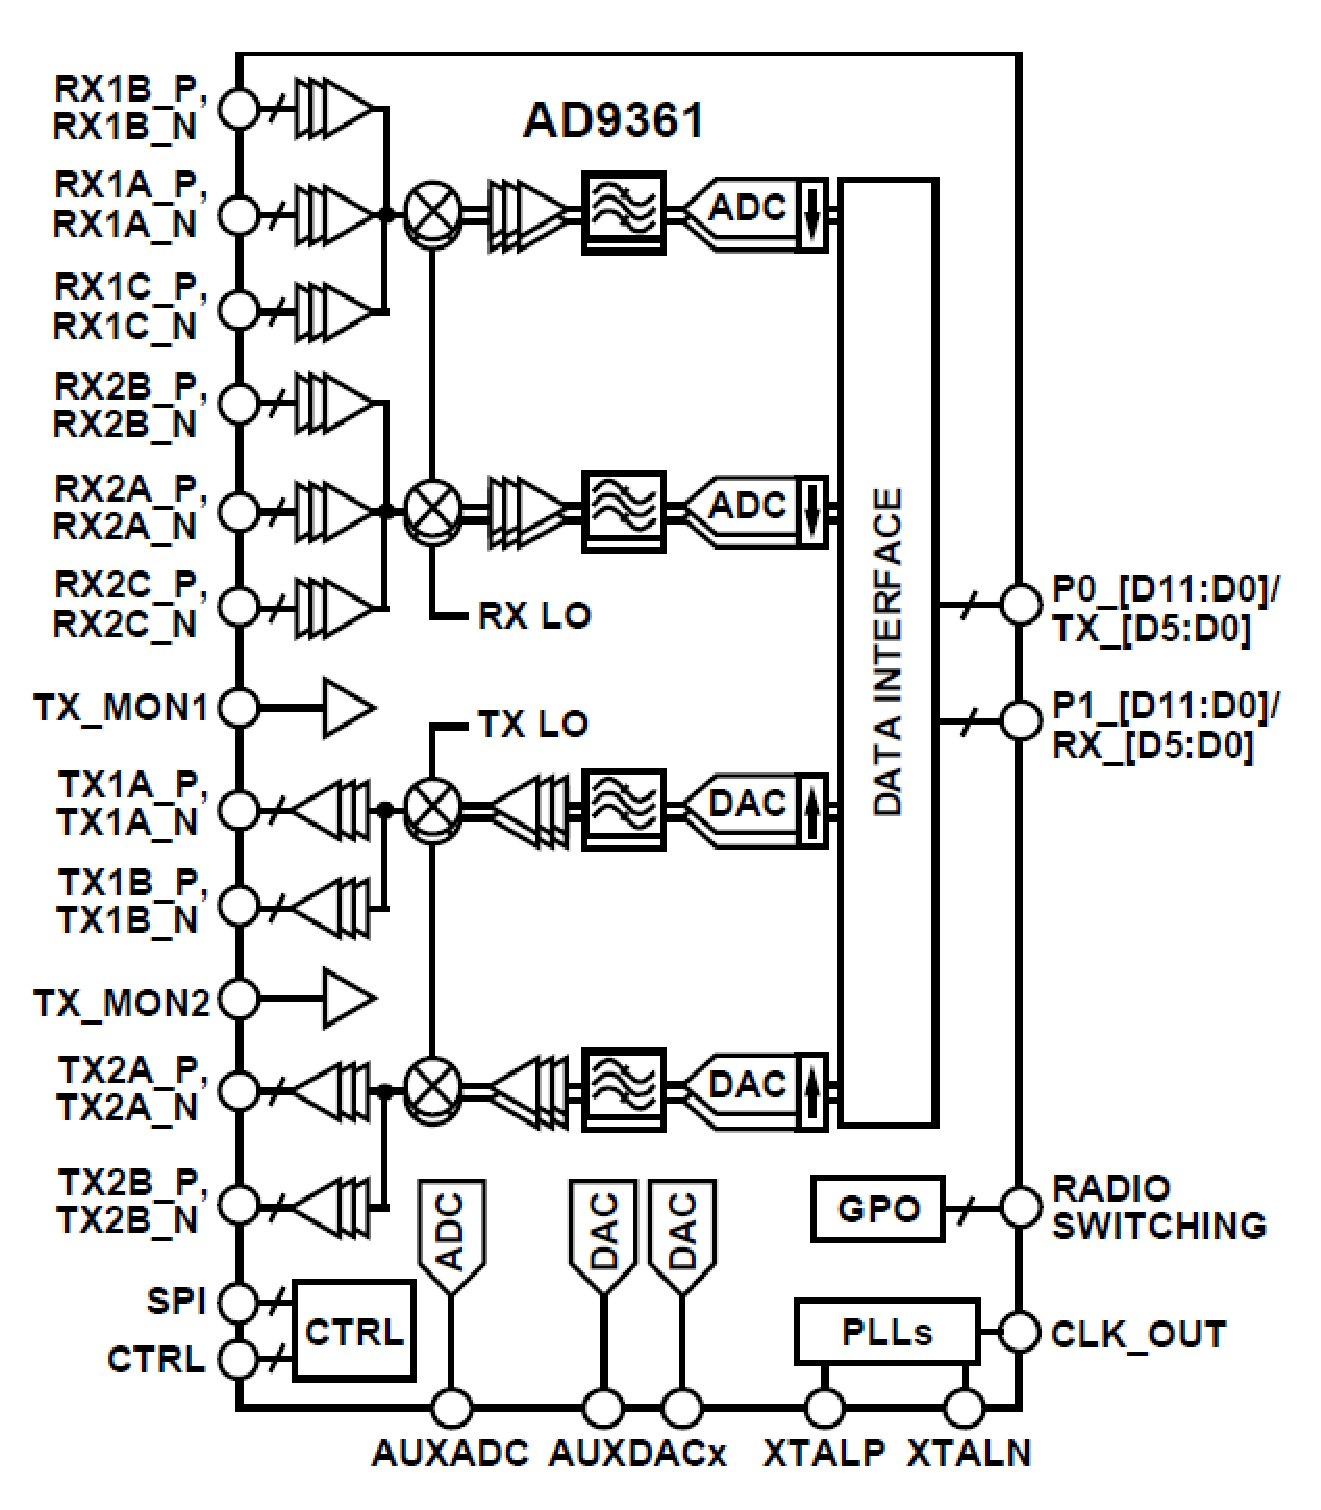
\includegraphics[width=0.45\textwidth]{./figures/ad9361_functional_diagram}
    \caption{ Image of the Setup Hardware
    \label{fig:setup}}
\end{figure}

\begin{figure}[htbp]
    \centering
    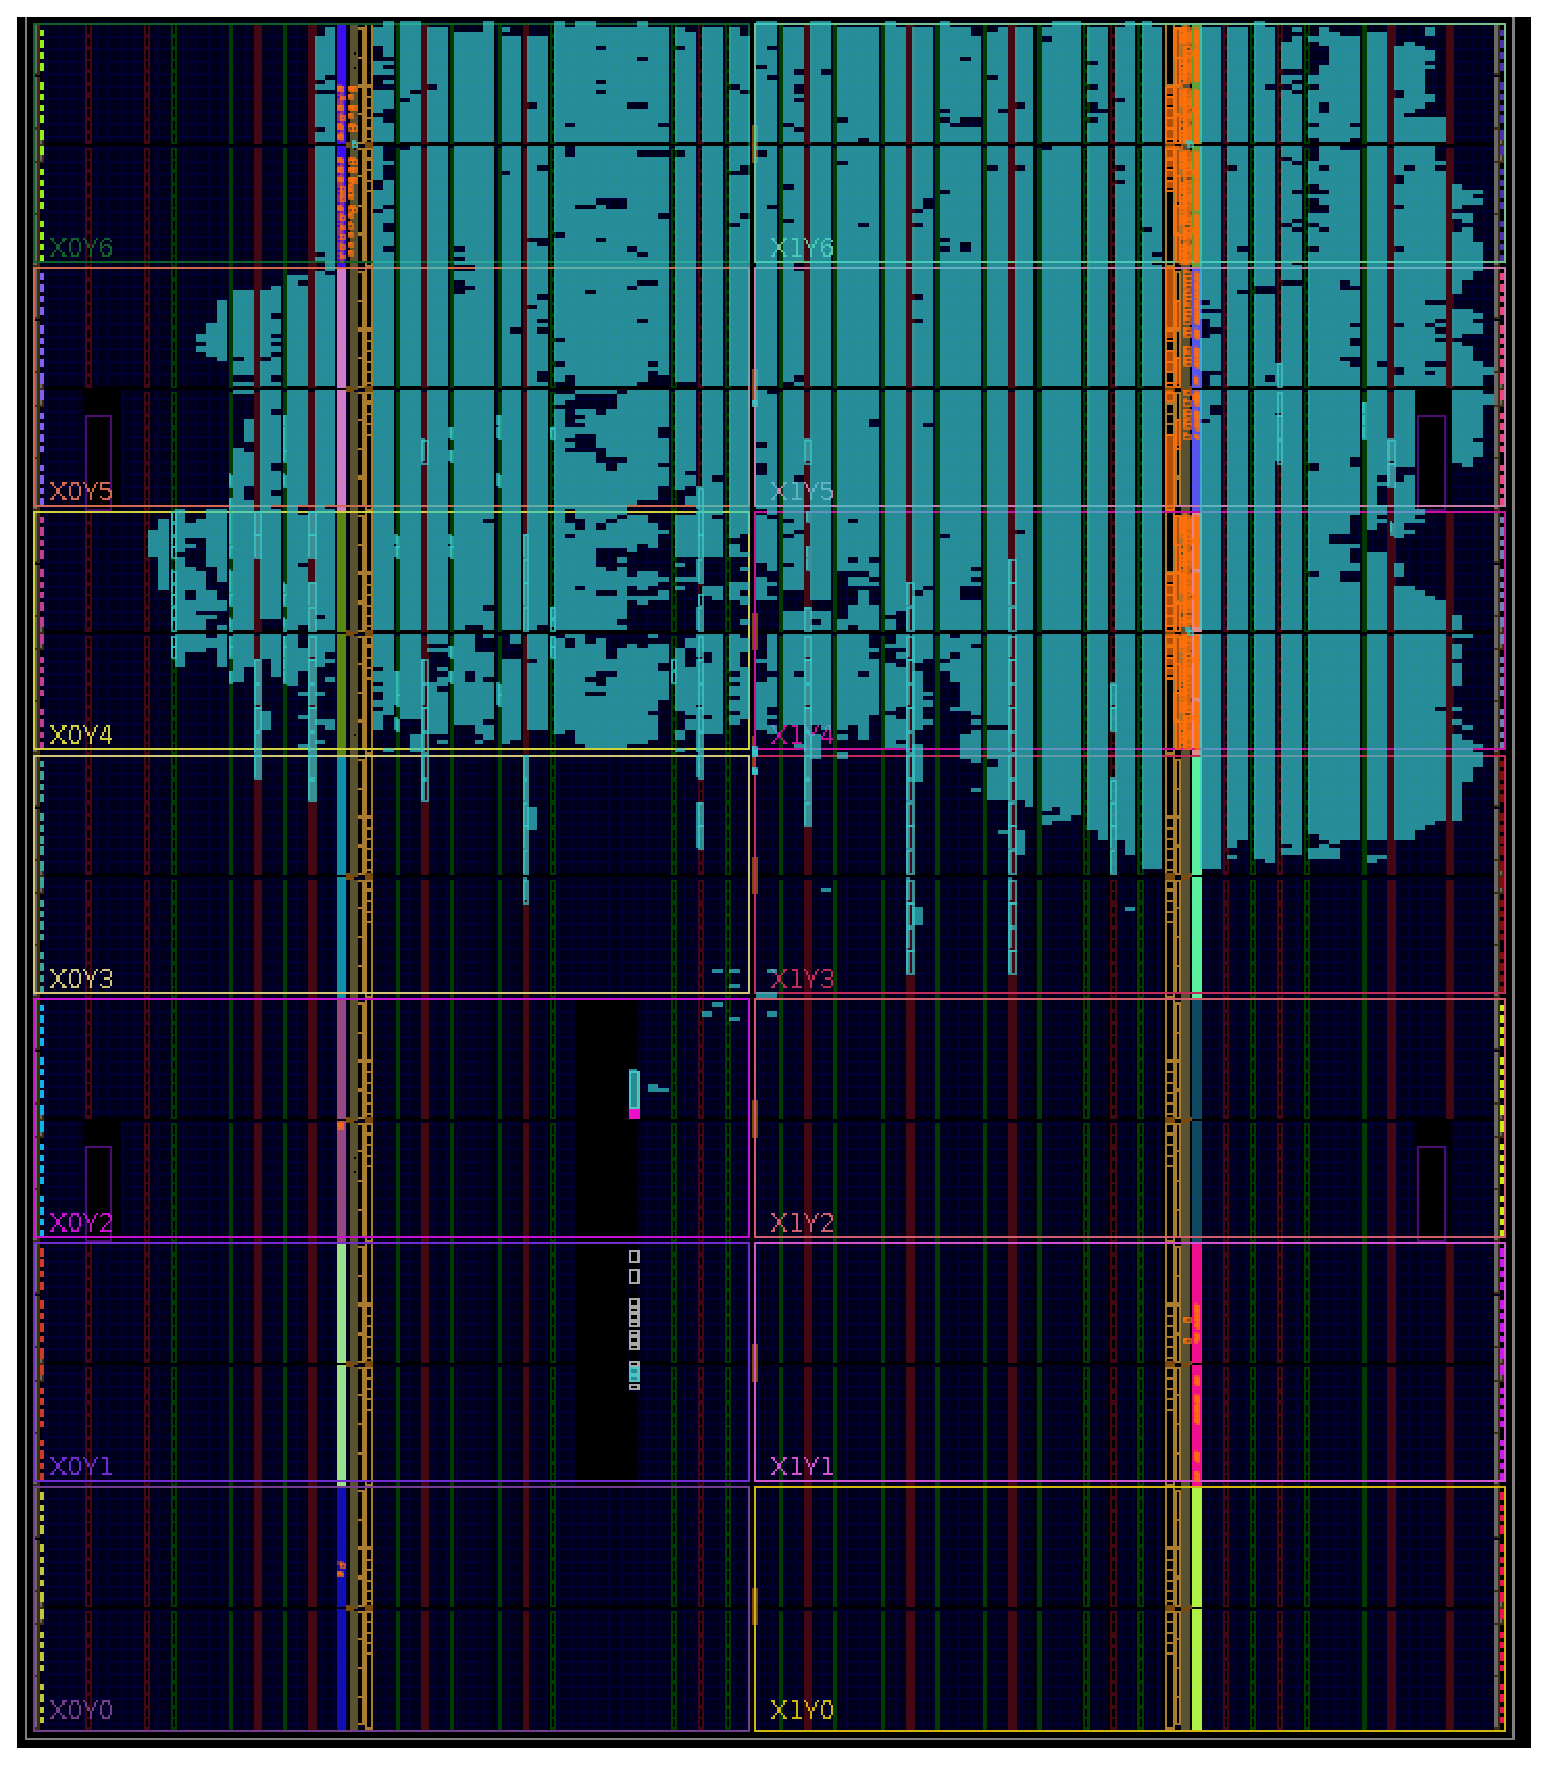
\includegraphics[width=0.35\textwidth]{./figures/fpga_area}
    \caption{ FPGA area used in this Setup
    \label{fig:fpgaarea}}
\end{figure}

%foto diagrama de blocos
\begin{figure}[htbp]
    \centering
    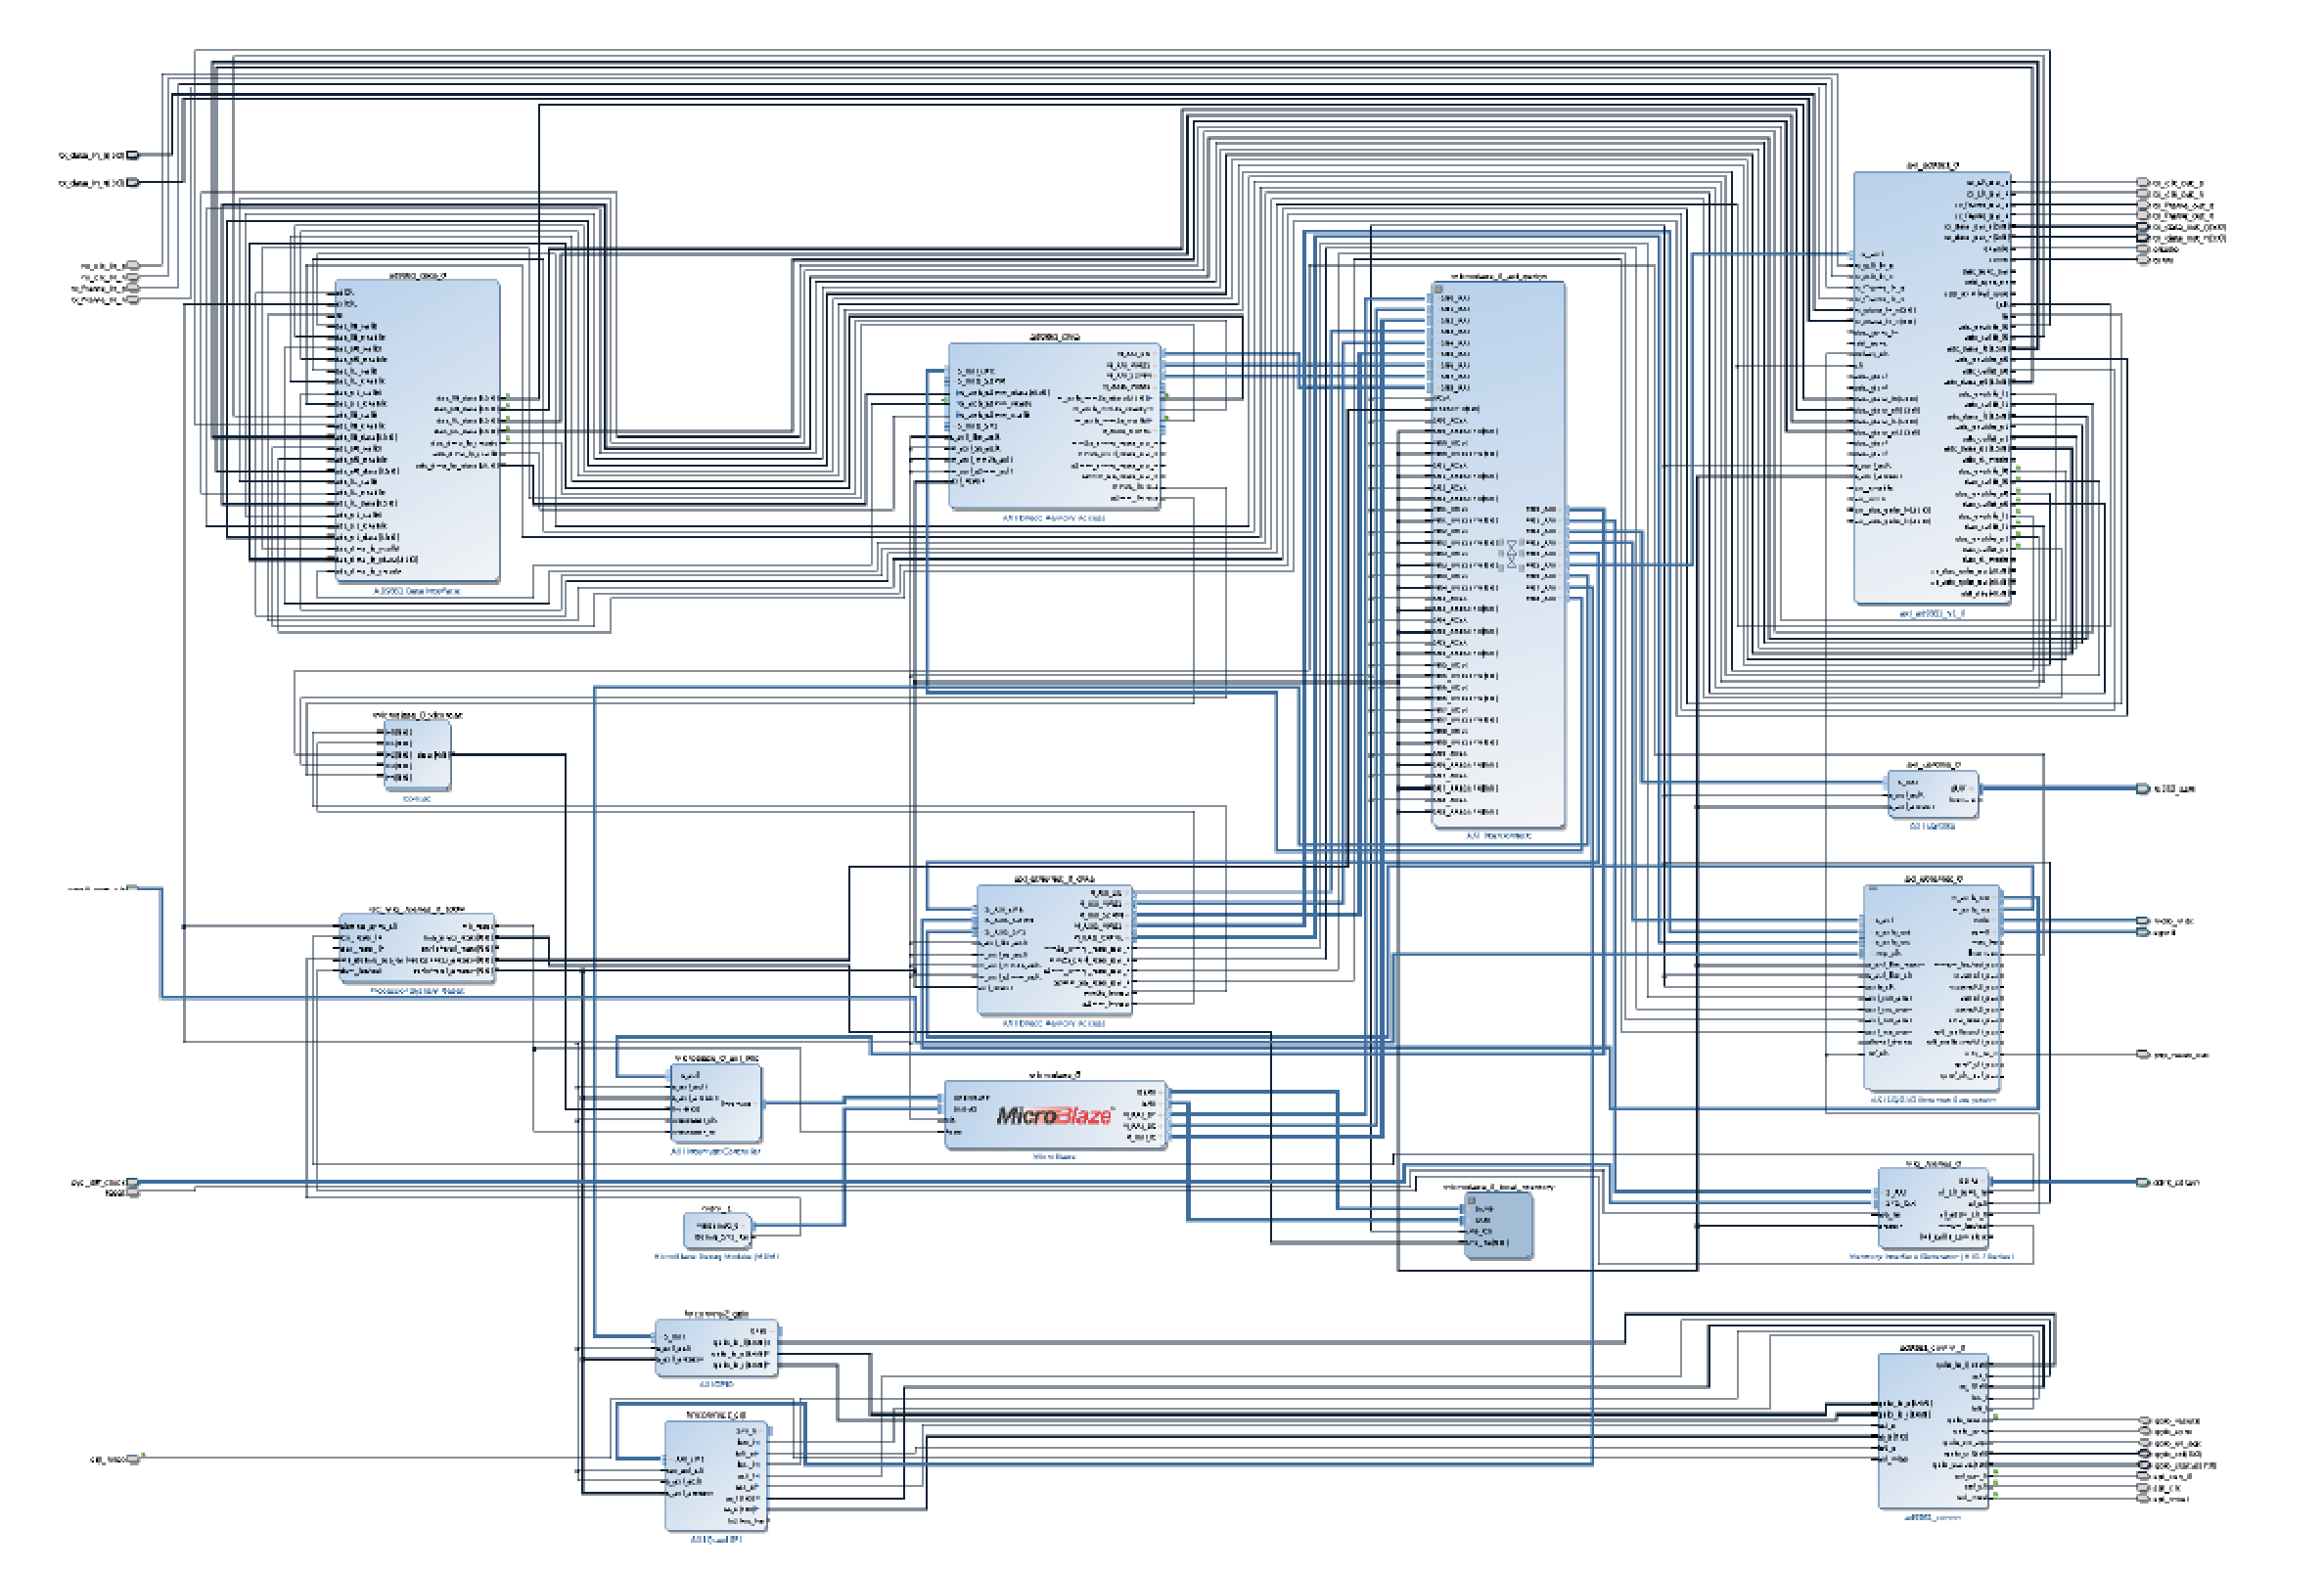
\includegraphics[width=0.95\textwidth]{./figures/setup_bd}
    \caption{ Image of the Setup Block diagram
    \label{fig:setupbd}}
\end{figure}

\vfill
\clearpage

\section{Preliminary Tests}
\label{result:conf}

The preliminary tests were focusing on initializing and communication between FPGA
and the FMComms2 board, in the previous chapter the steps of setting up communication
and control interface were described, and it describes also how this interface works
and how a block was made to implement such, in short it was needed to set up SPI and GPIO
modules and make the right input and output ports specified in \ref{subs:controlif} and
after the initialization and callibration is finished, it is possible to observ the
carrier wave centralized at the frequency 2.4 Ghz.

To generate the outputs two analyzers were used, one oscilloscope and one spectrum analyzer,
both analyzers outputs can be seen in the figures below:

%spectrum analyser image
\begin{figure}[htbp]
    \centering
    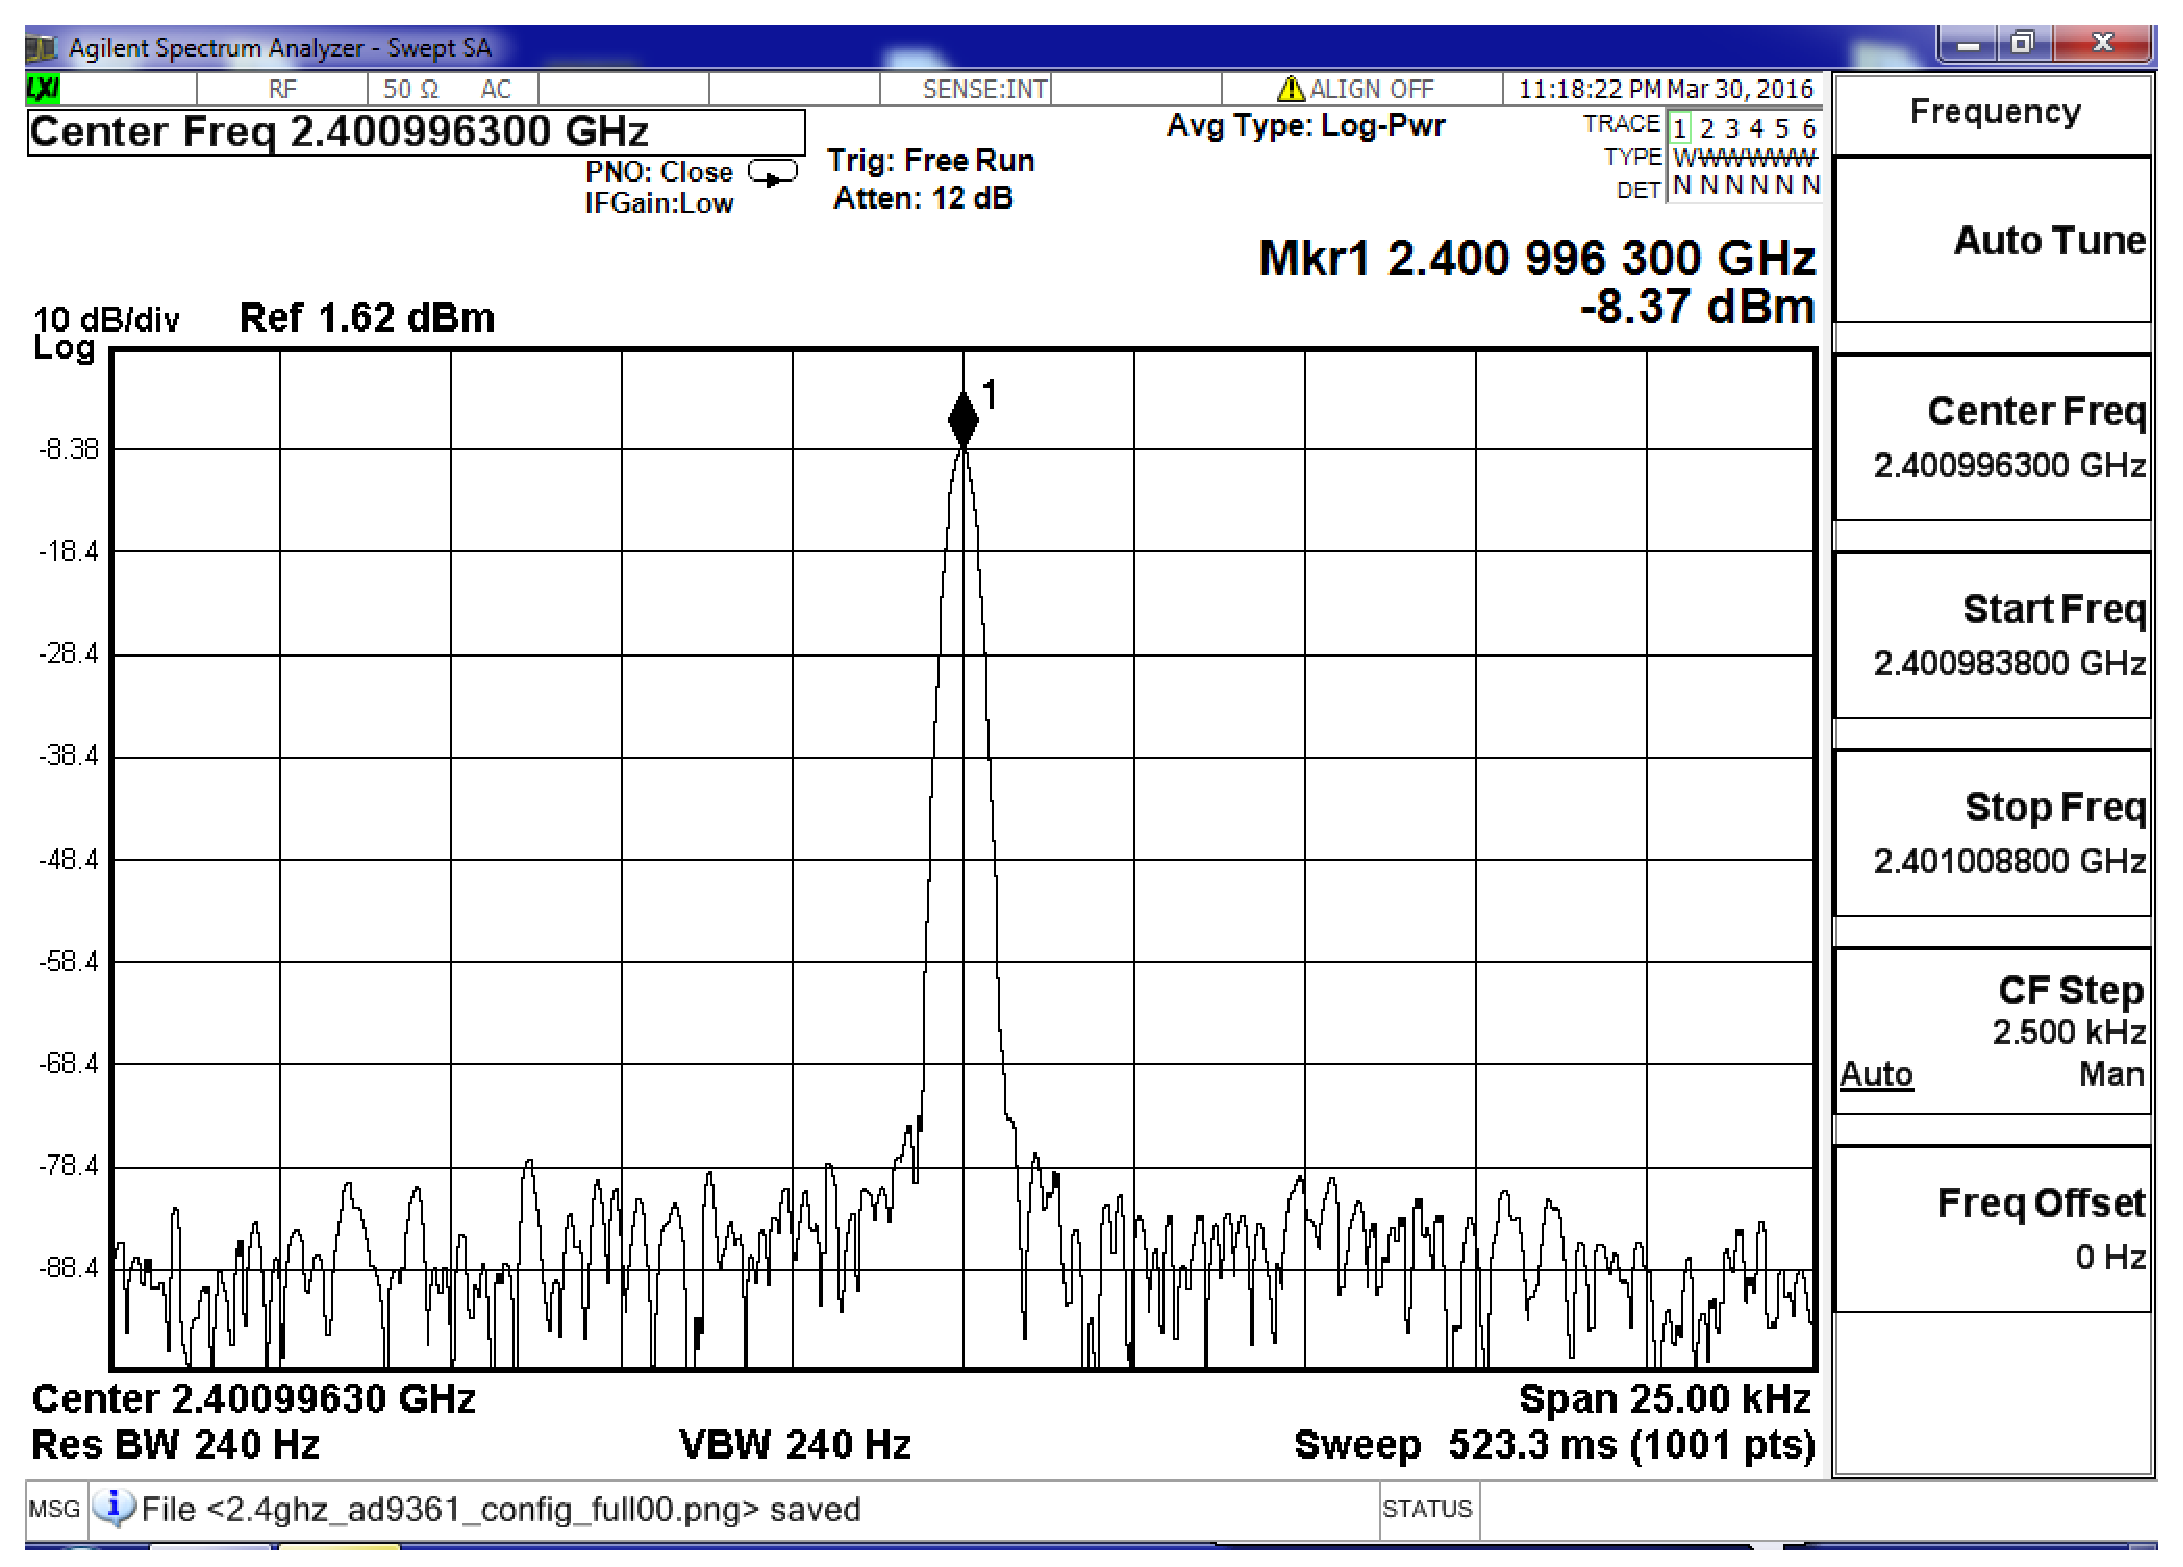
\includegraphics[width=0.85\textwidth]{./figures/spectrum_init}
    \caption{ Spectrum Analyzer Screen
    \label{fig:spec}}
\end{figure}

%initialization
\begin{figure}[htbp]
    \centering
    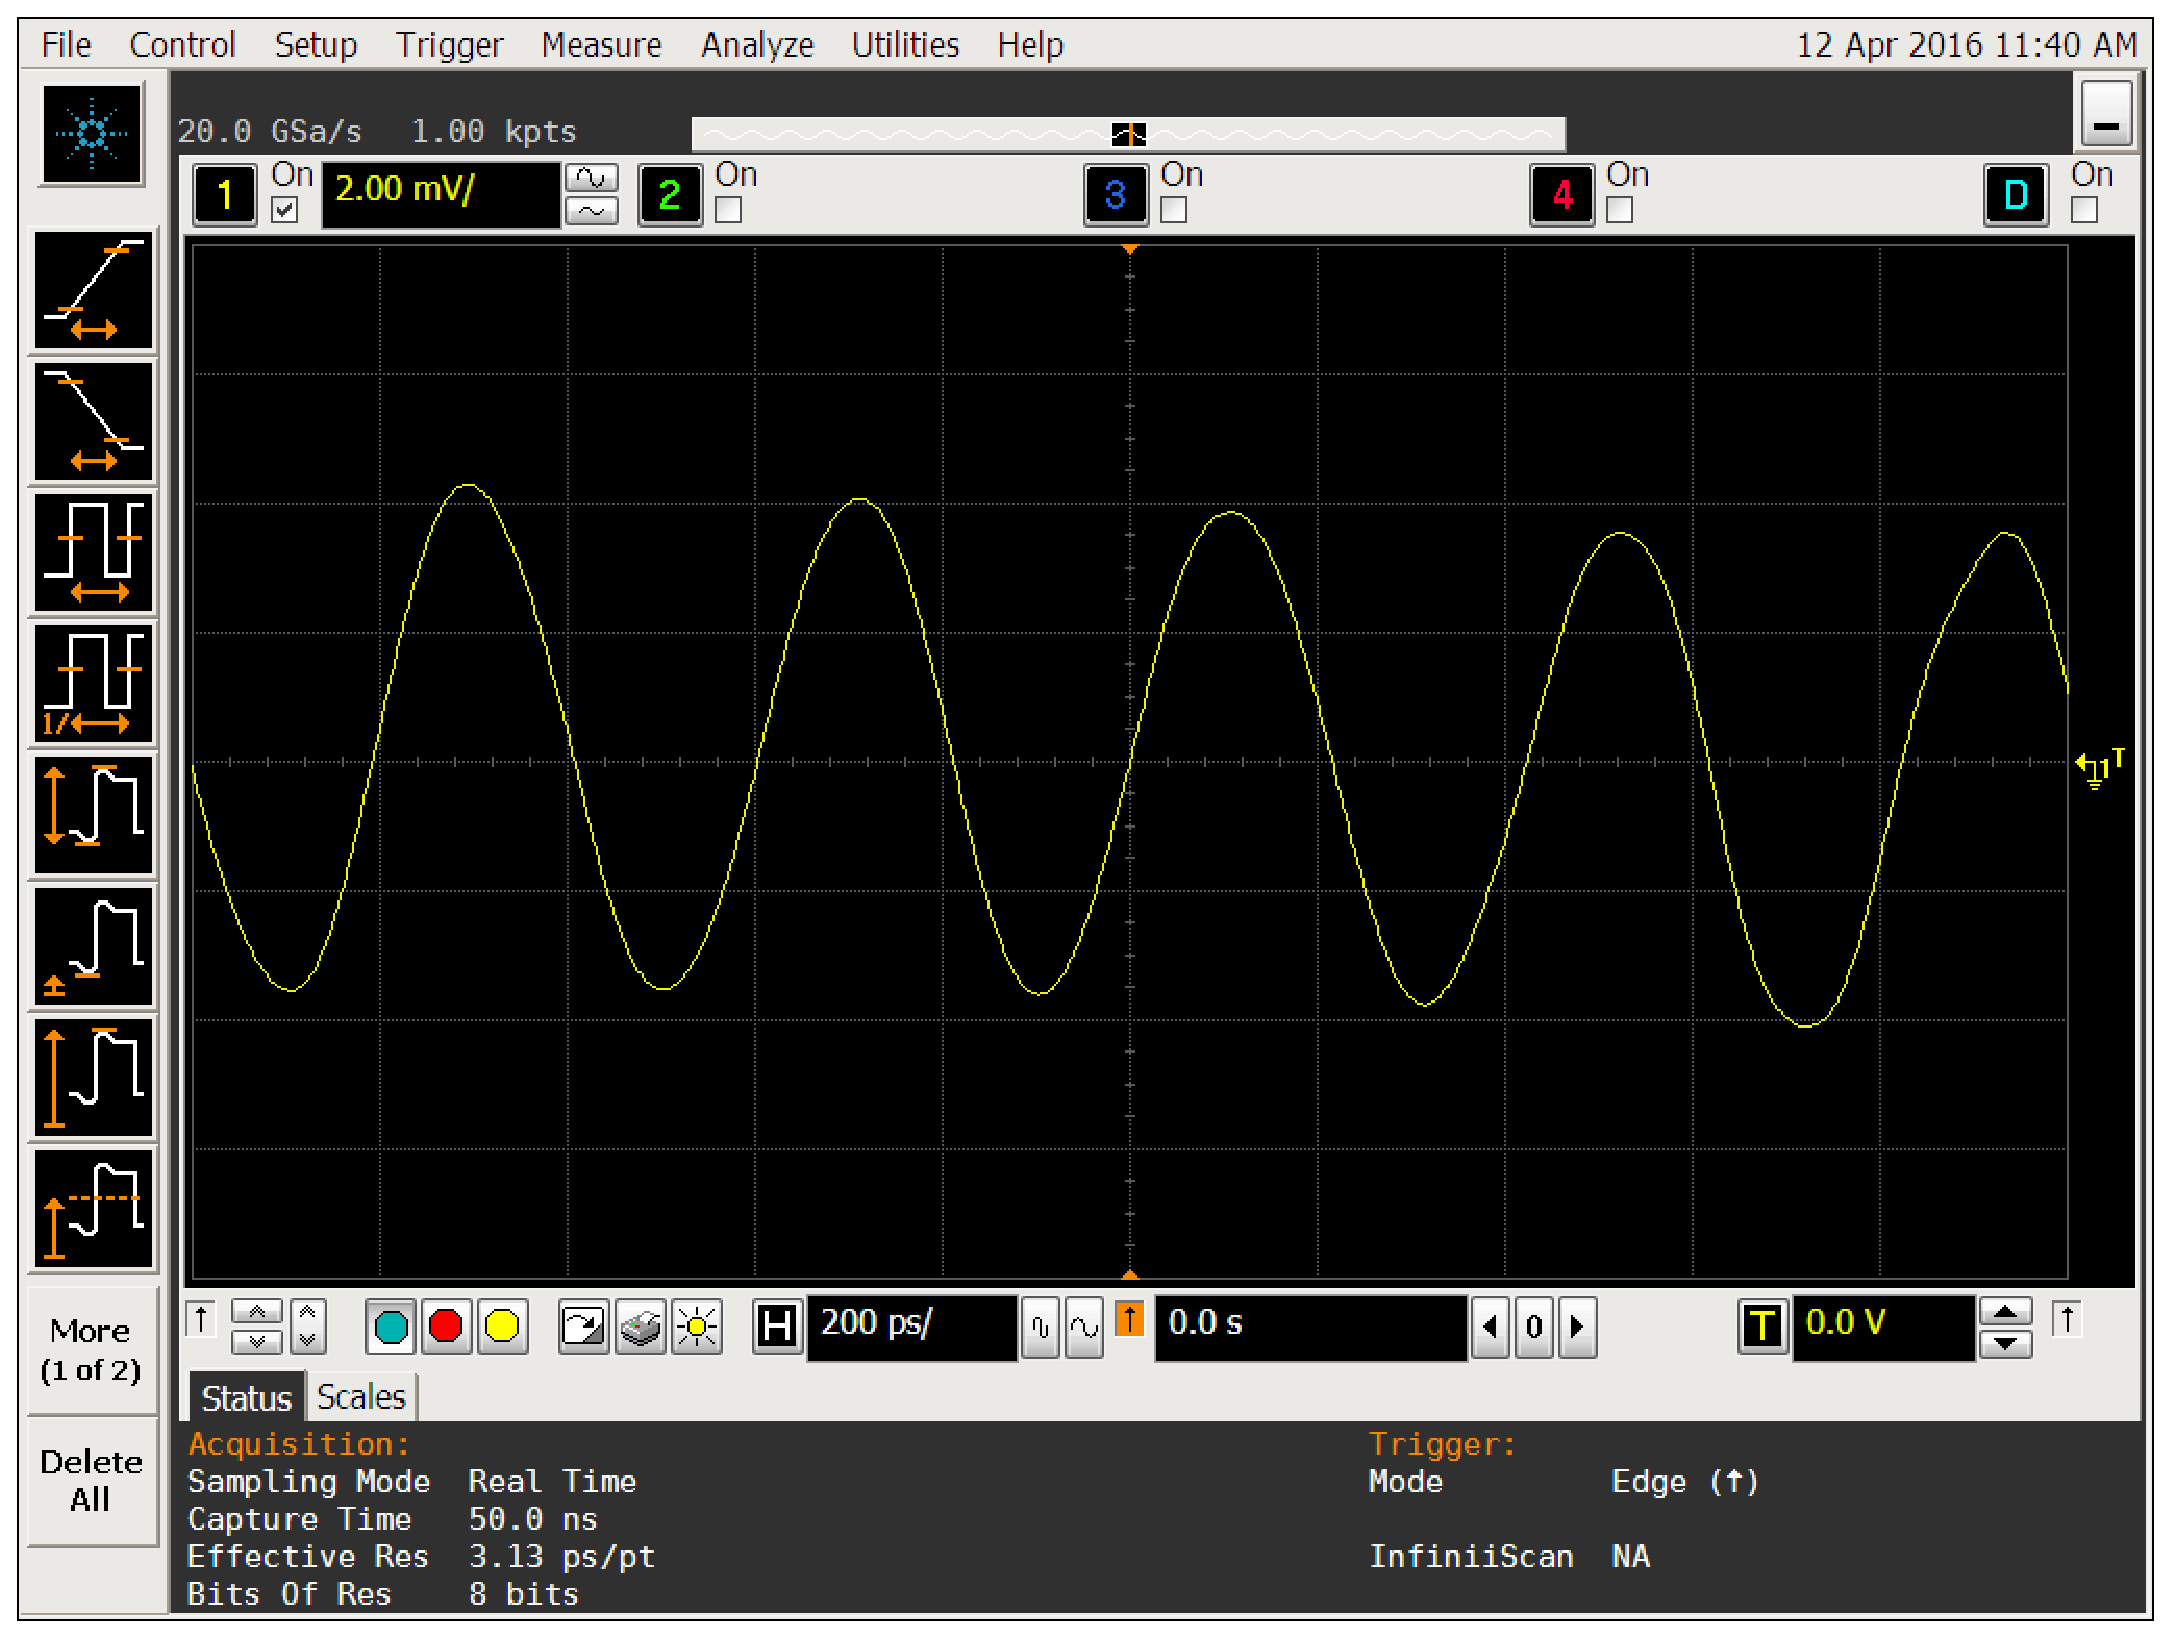
\includegraphics[width=0.85\textwidth]{./figures/oscill_init}
    \caption{ Carrier Waveform after Initialization
    \label{fig:oscillinit}}
\end{figure}

%digital tune
\begin{figure}[htbp]
    \centering
    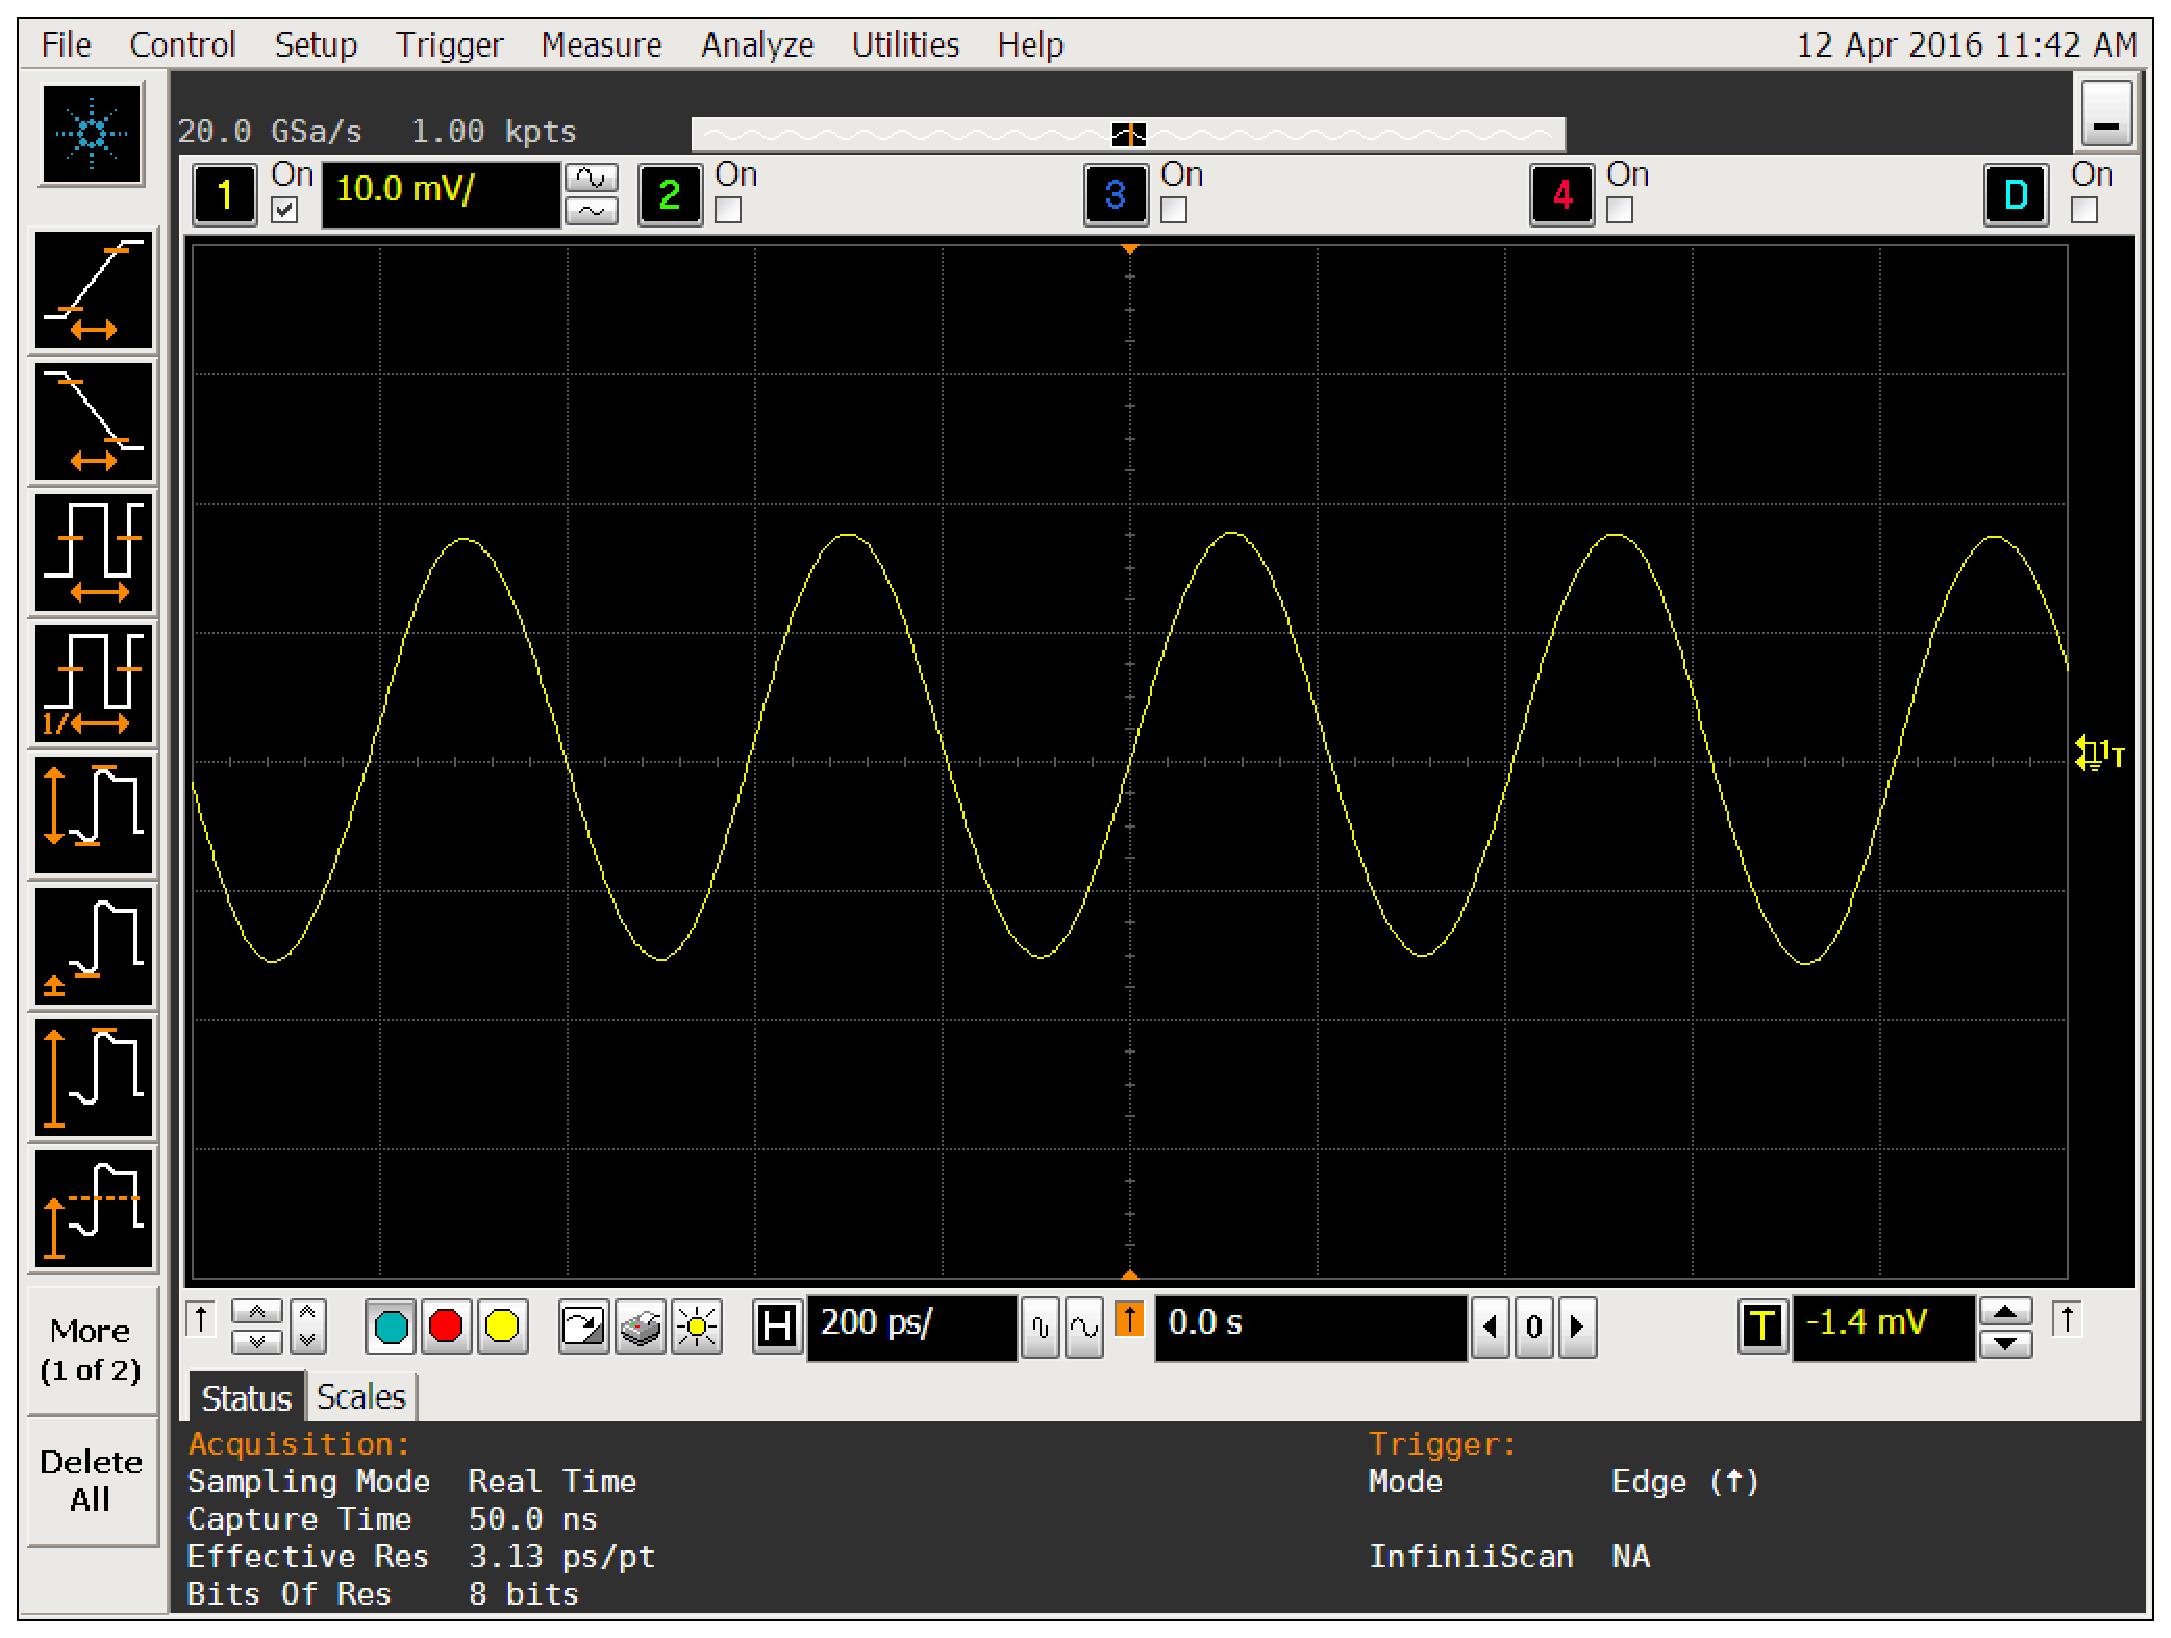
\includegraphics[width=0.85\textwidth]{./figures/oscill_dig}
    \caption{ Carrier Waveform after Tunning Digital Interface
    \label{fig:oscilldig}}
\end{figure}

%freq
\begin{figure}[htbp]
    \centering
    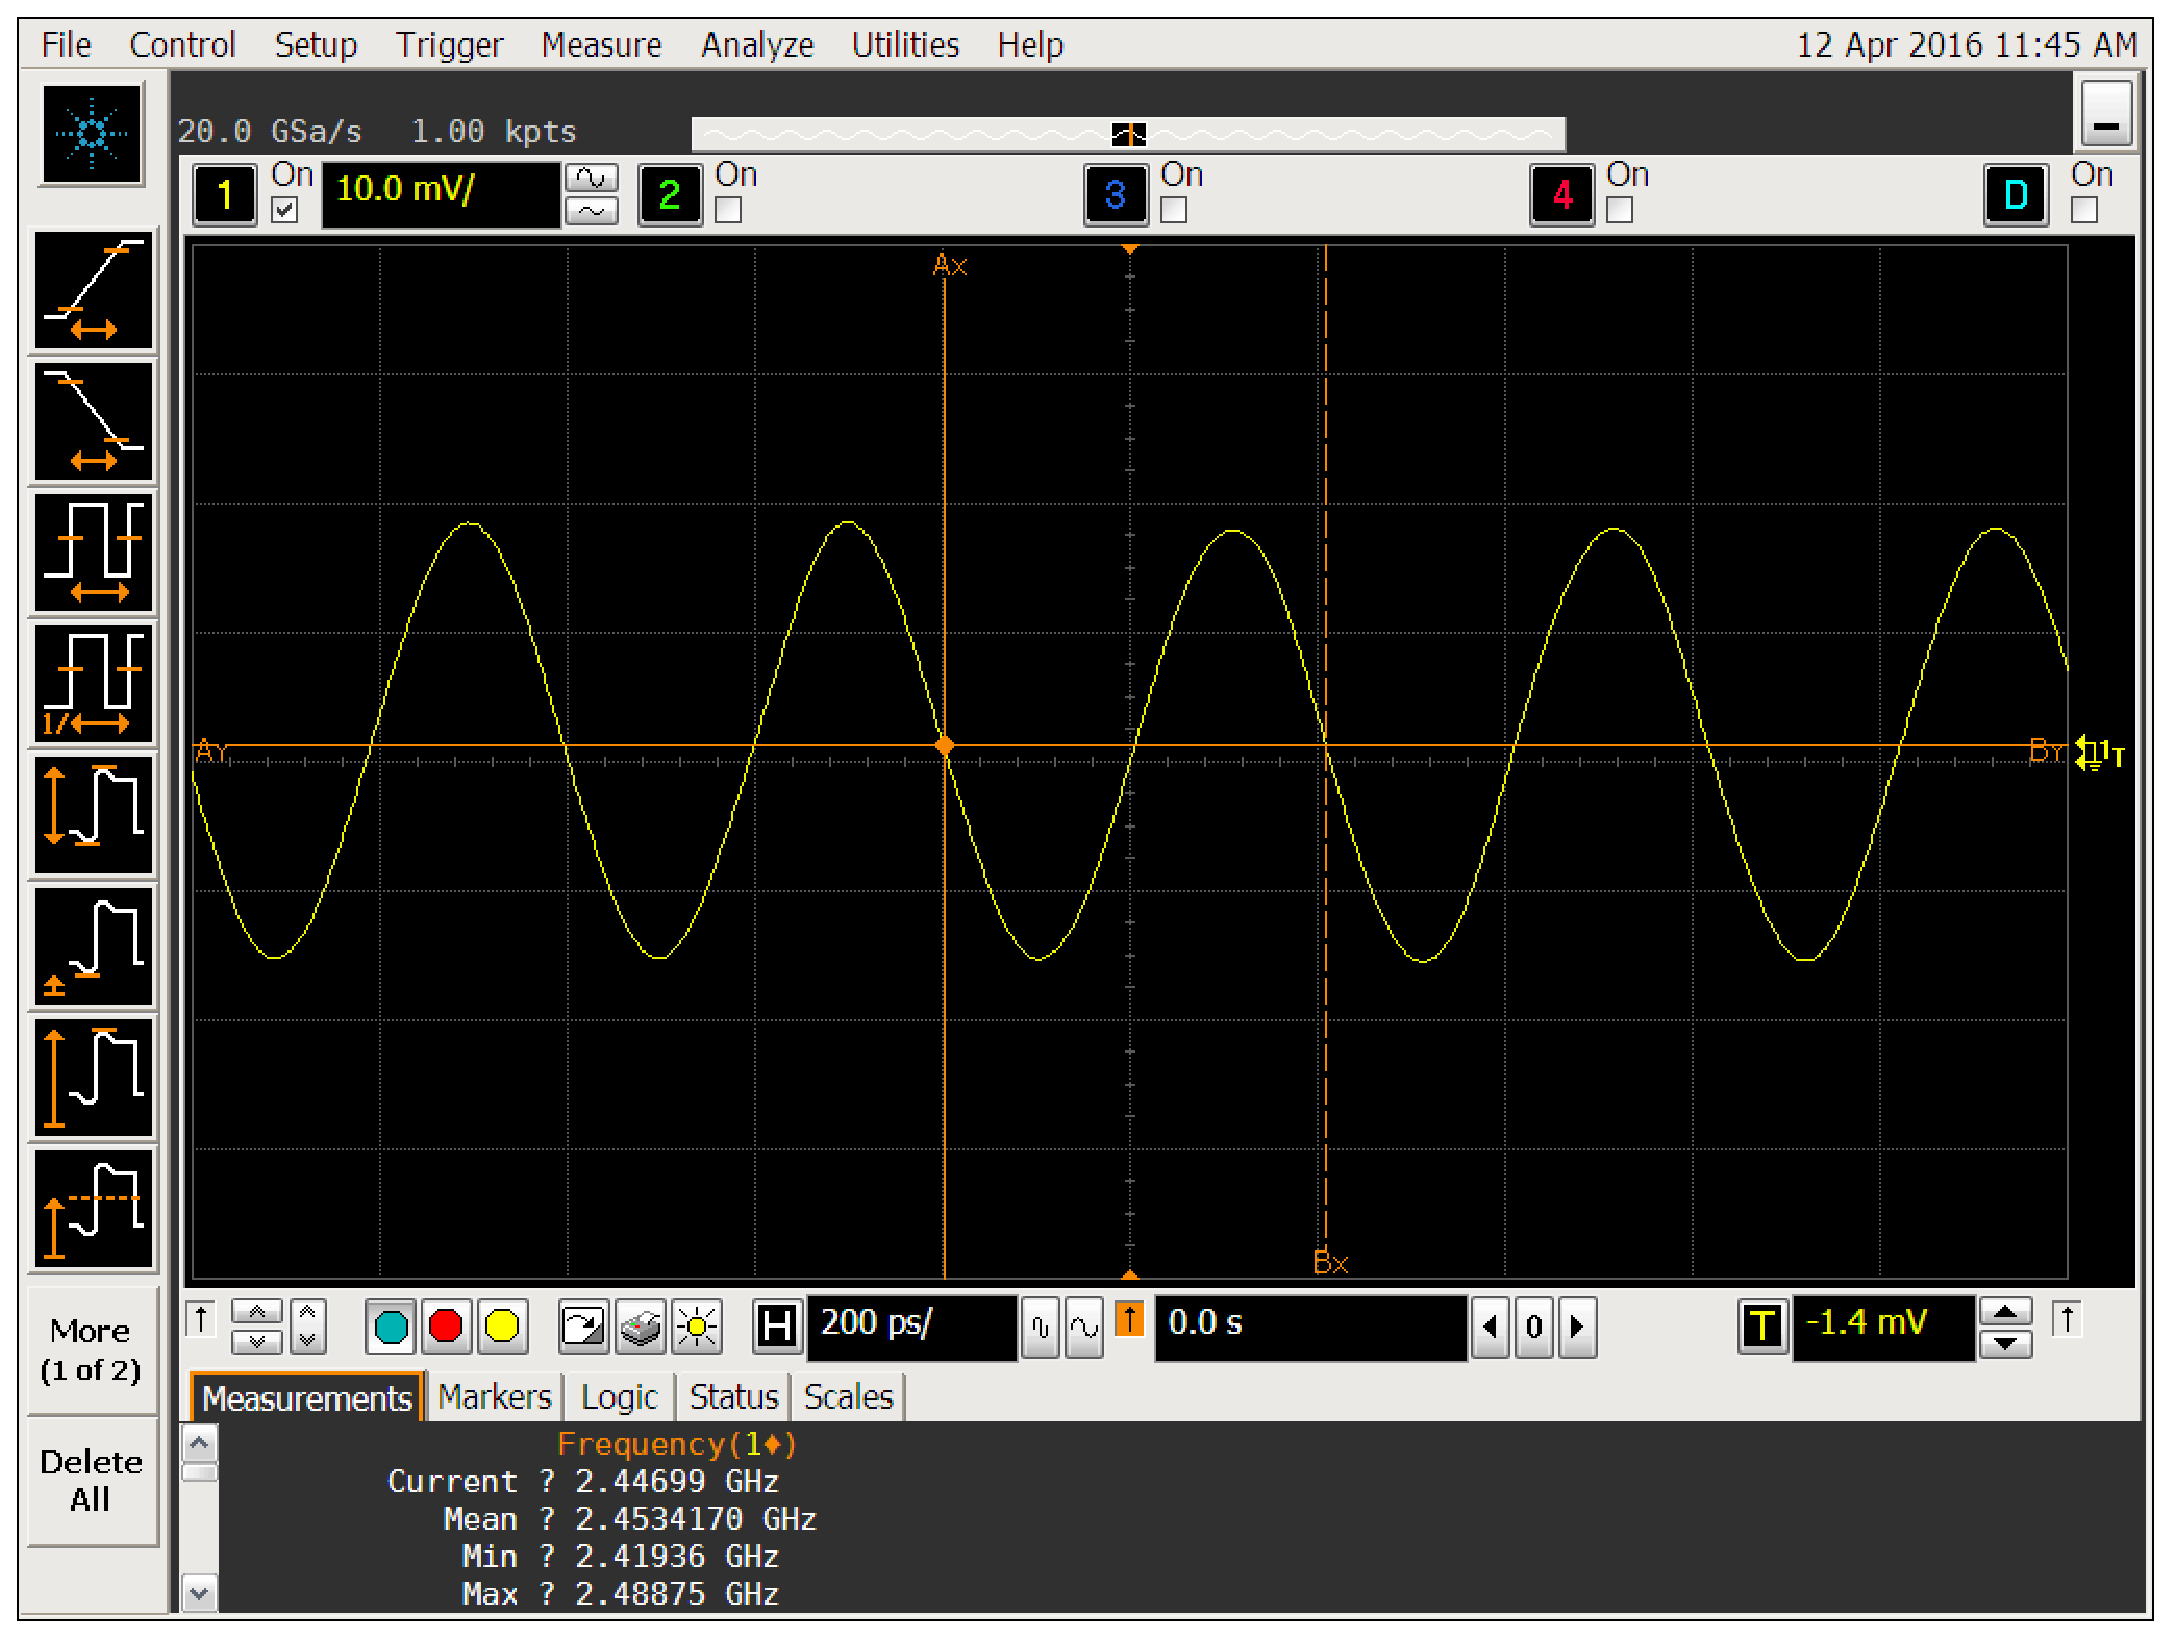
\includegraphics[width=0.85\textwidth]{./figures/oscill_freq}
    \caption{ Carrier Waveform with Frequency Measure
    \label{fig:oscillfreq}}
\end{figure}

%fft config
\begin{figure}[htbp]
    \centering
    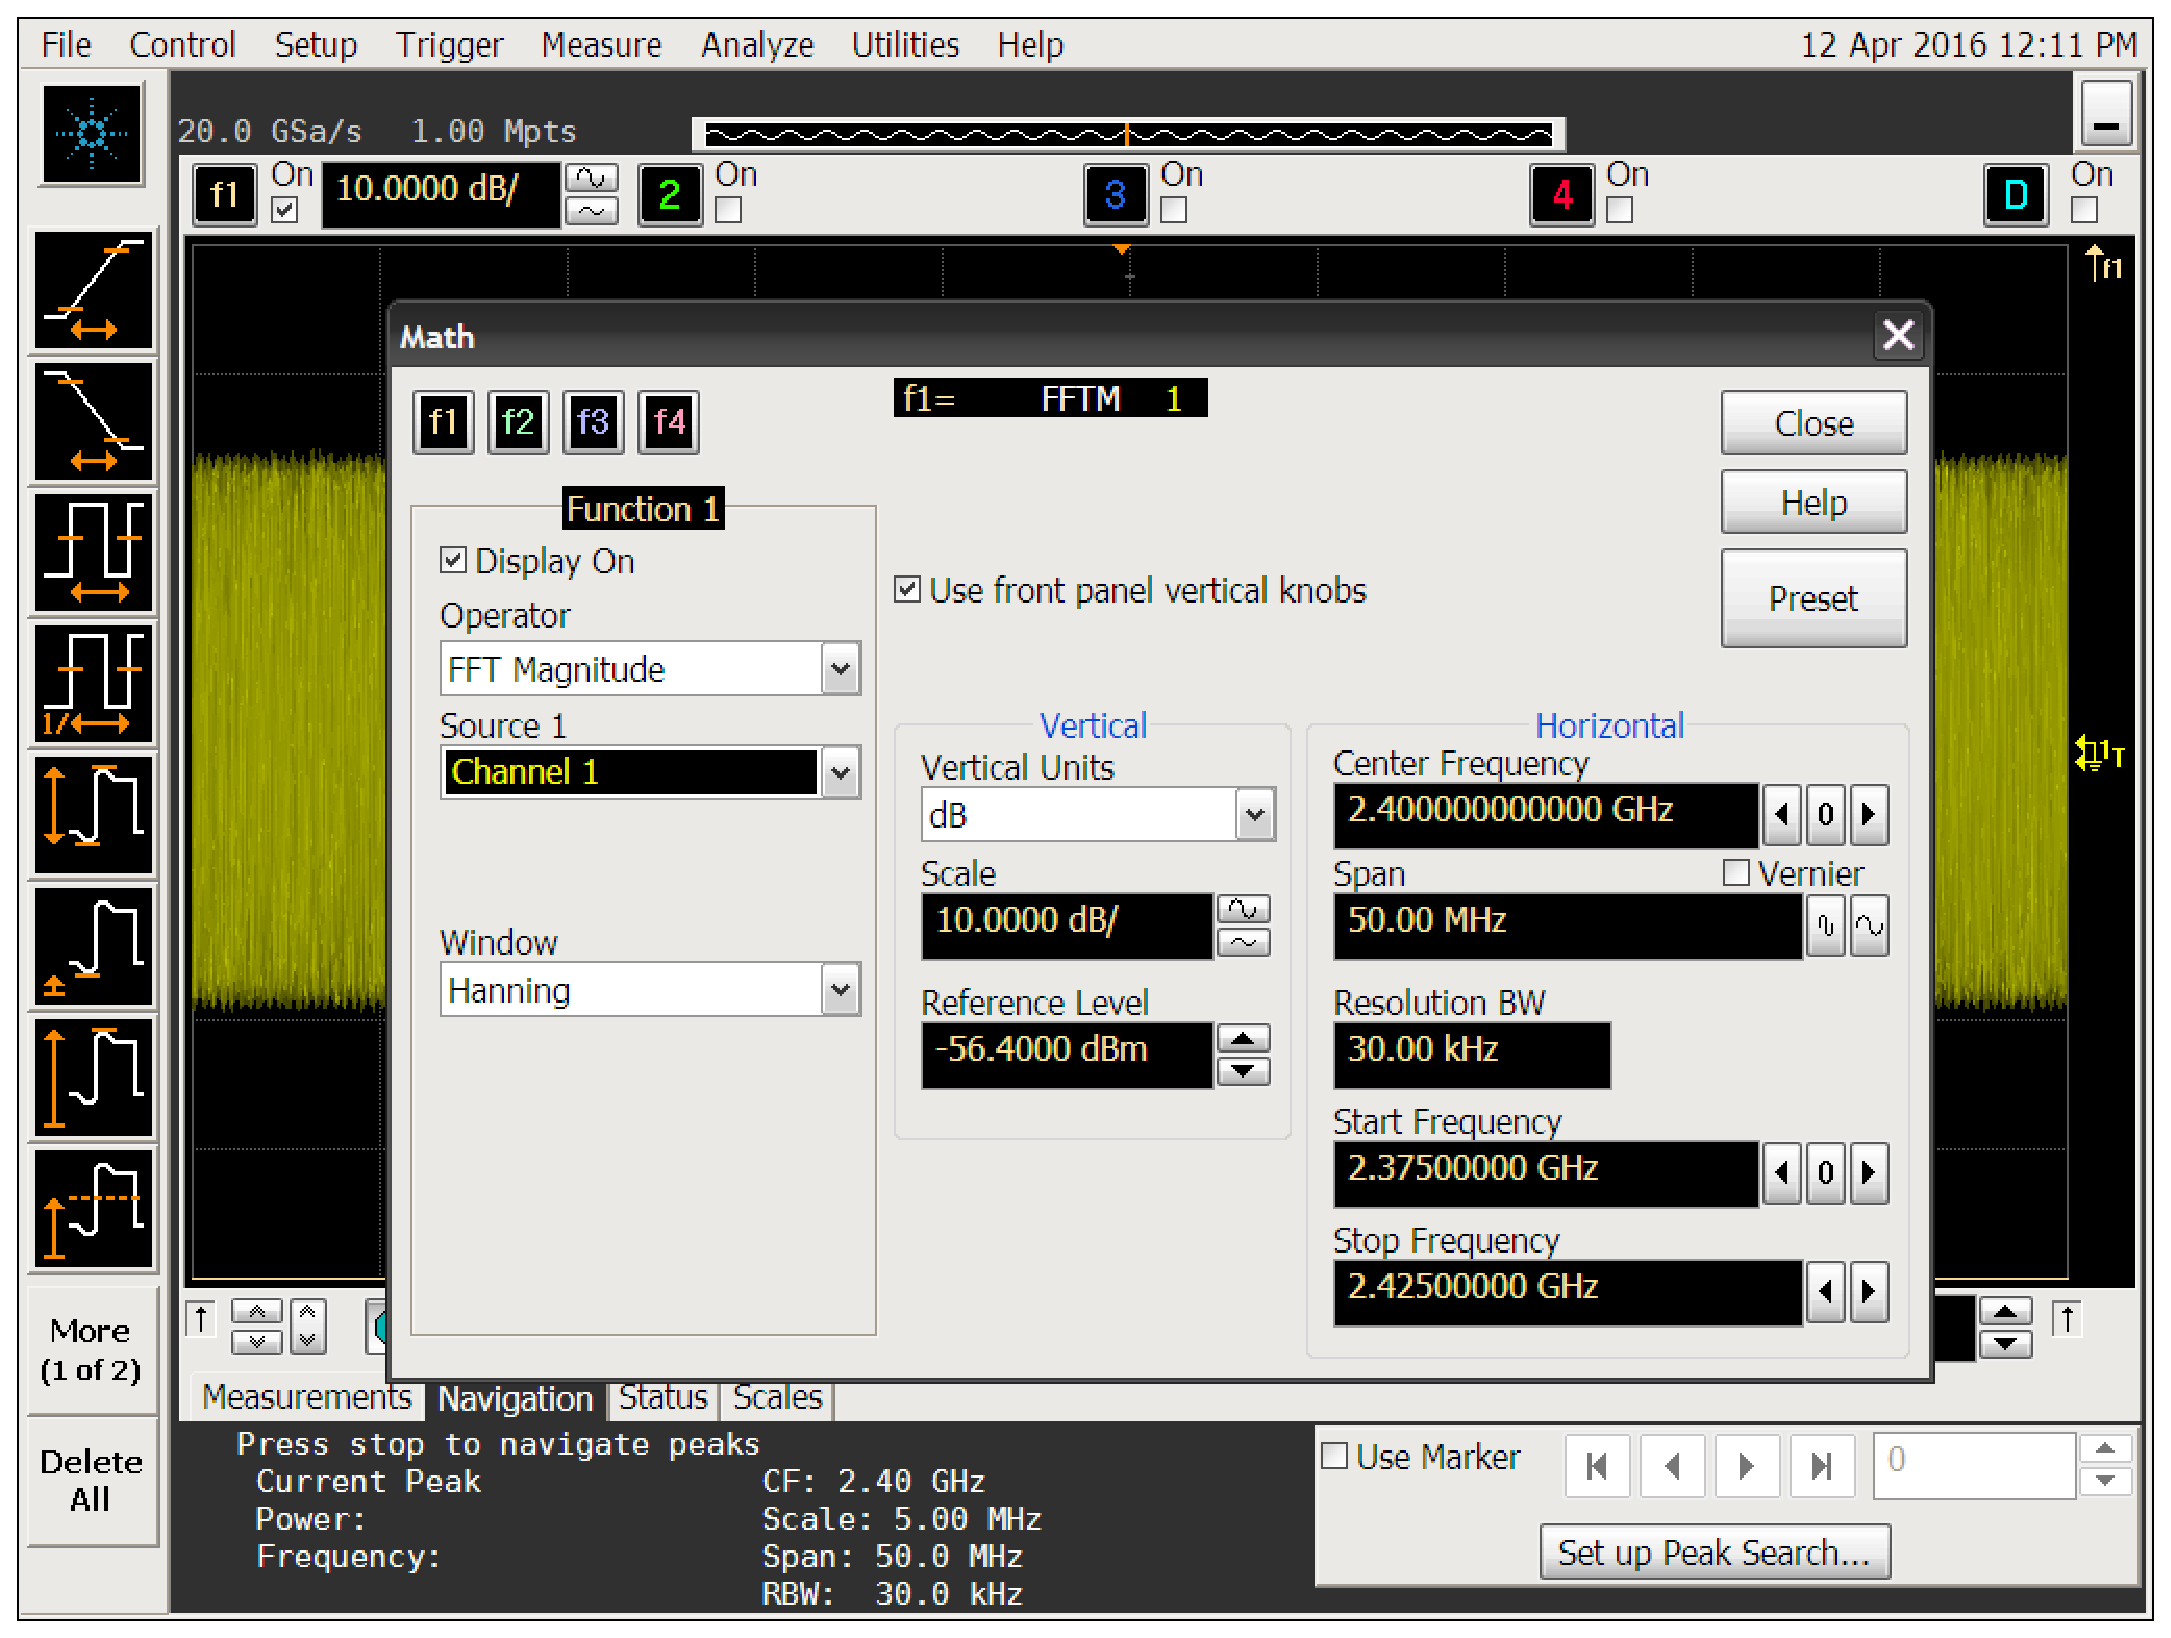
\includegraphics[width=0.85\textwidth]{./figures/oscill_fftcf}
    \caption{ FFT Configuration Parameters
    \label{fig:oscillfftcf}}
\end{figure}

%wave + fft
\begin{figure}[htbp]
    \centering
    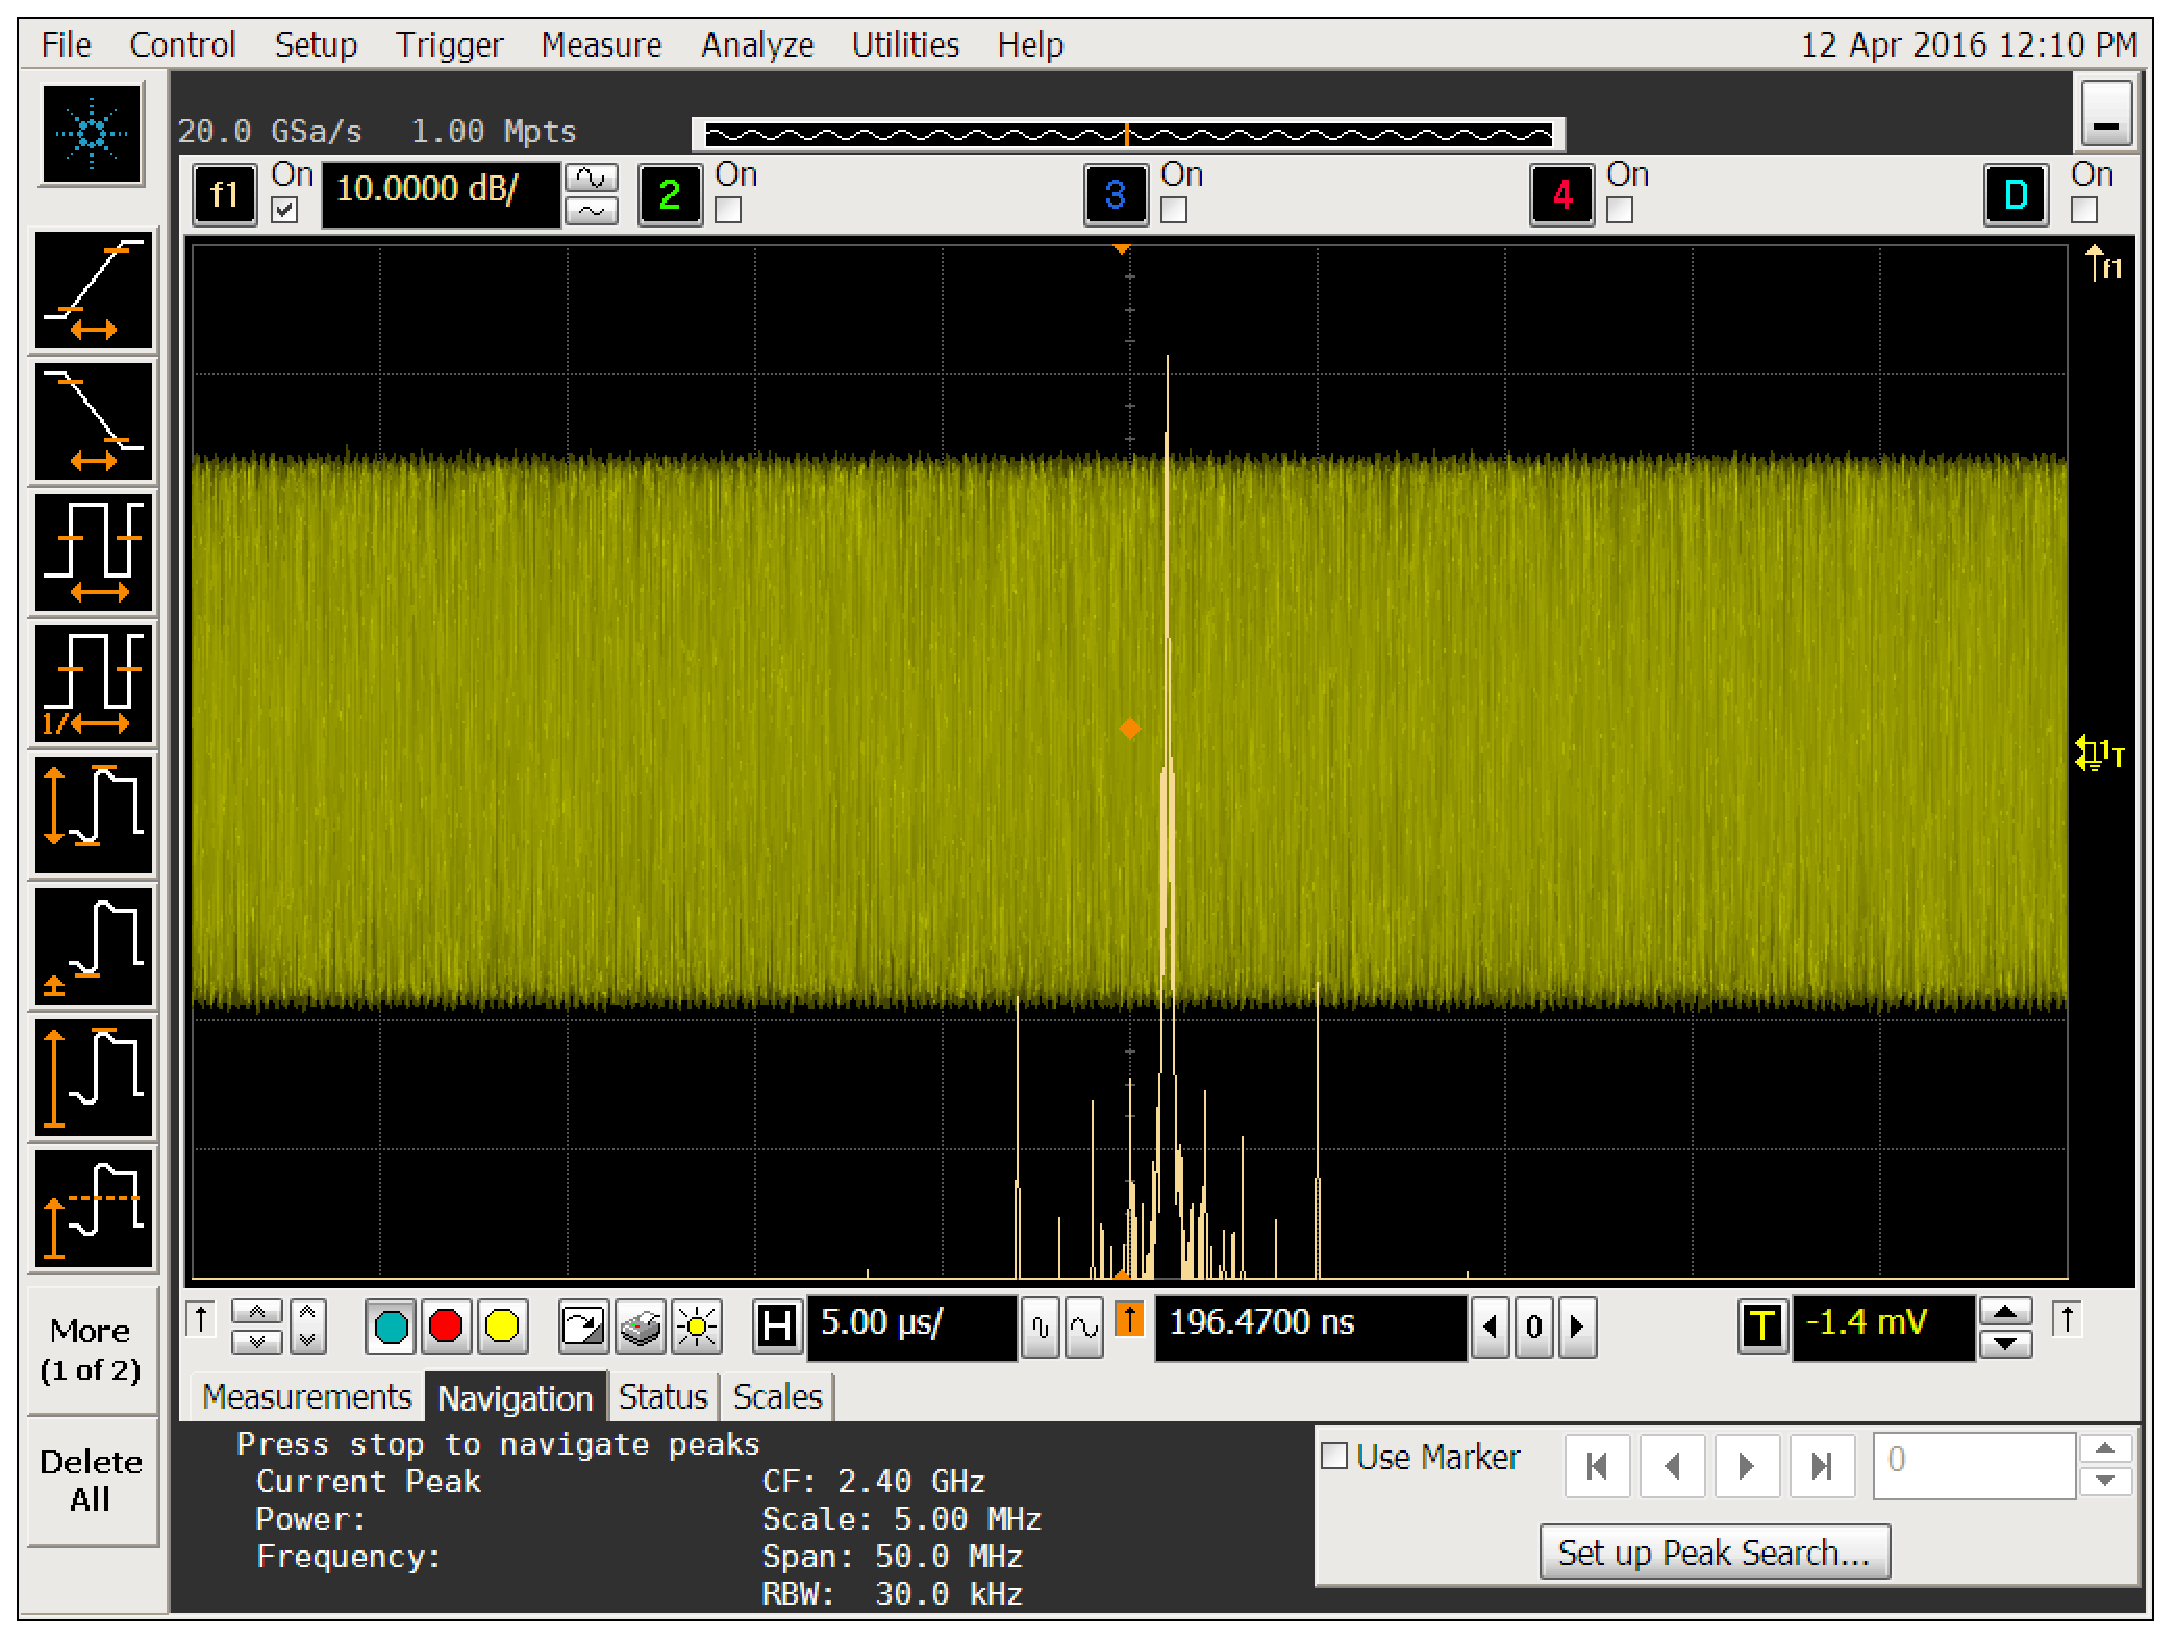
\includegraphics[width=0.85\textwidth]{./figures/oscill_fft}
    \caption{ FFT and Carrier Waveform
    \label{fig:oscillfft}}
\end{figure}

\vfill
\clearpage

\section{Simulation}

An important step in HDL development is the logic simulation of the circuit,
through this simulation it is possible to watch every port and be able to
understand the block behavior, thus correcting any problem or misbehavior.

\subsection{Transmit (DAC) Interface Simulation}

The simulation of the transmit interface, which interfaces the FPGA with DAC was
made in three steps, since the interface is composed by two blocks, there was
the need to simulate each block separately and after this simulate both blocks
connected and working together, in the figures \ref{fig:simdacdma},
\ref{fig:simdac} and \ref{fig:simtxif} it is possible to see the simulation
results and wave diagrams of the three steps.

In the figure \ref{fig:simdacdma} it is possible to watch the behavior of the
\textit{dac-dmaIterface} block where the signal \textit{sig\_dma\_data} is fed to
the block, and the signals \textit{ sig\_axis\_axc0\_itdata, sig\_axis\_axc0\_qtdata,
sig\_axis\_axc1\_itdata and sig\_axis\_axc1\_qtdata} are the \textit{IQ data} being
fed to both to the \textit{dacInterface} block.

\begin{figure}[htbp]
    \centering
    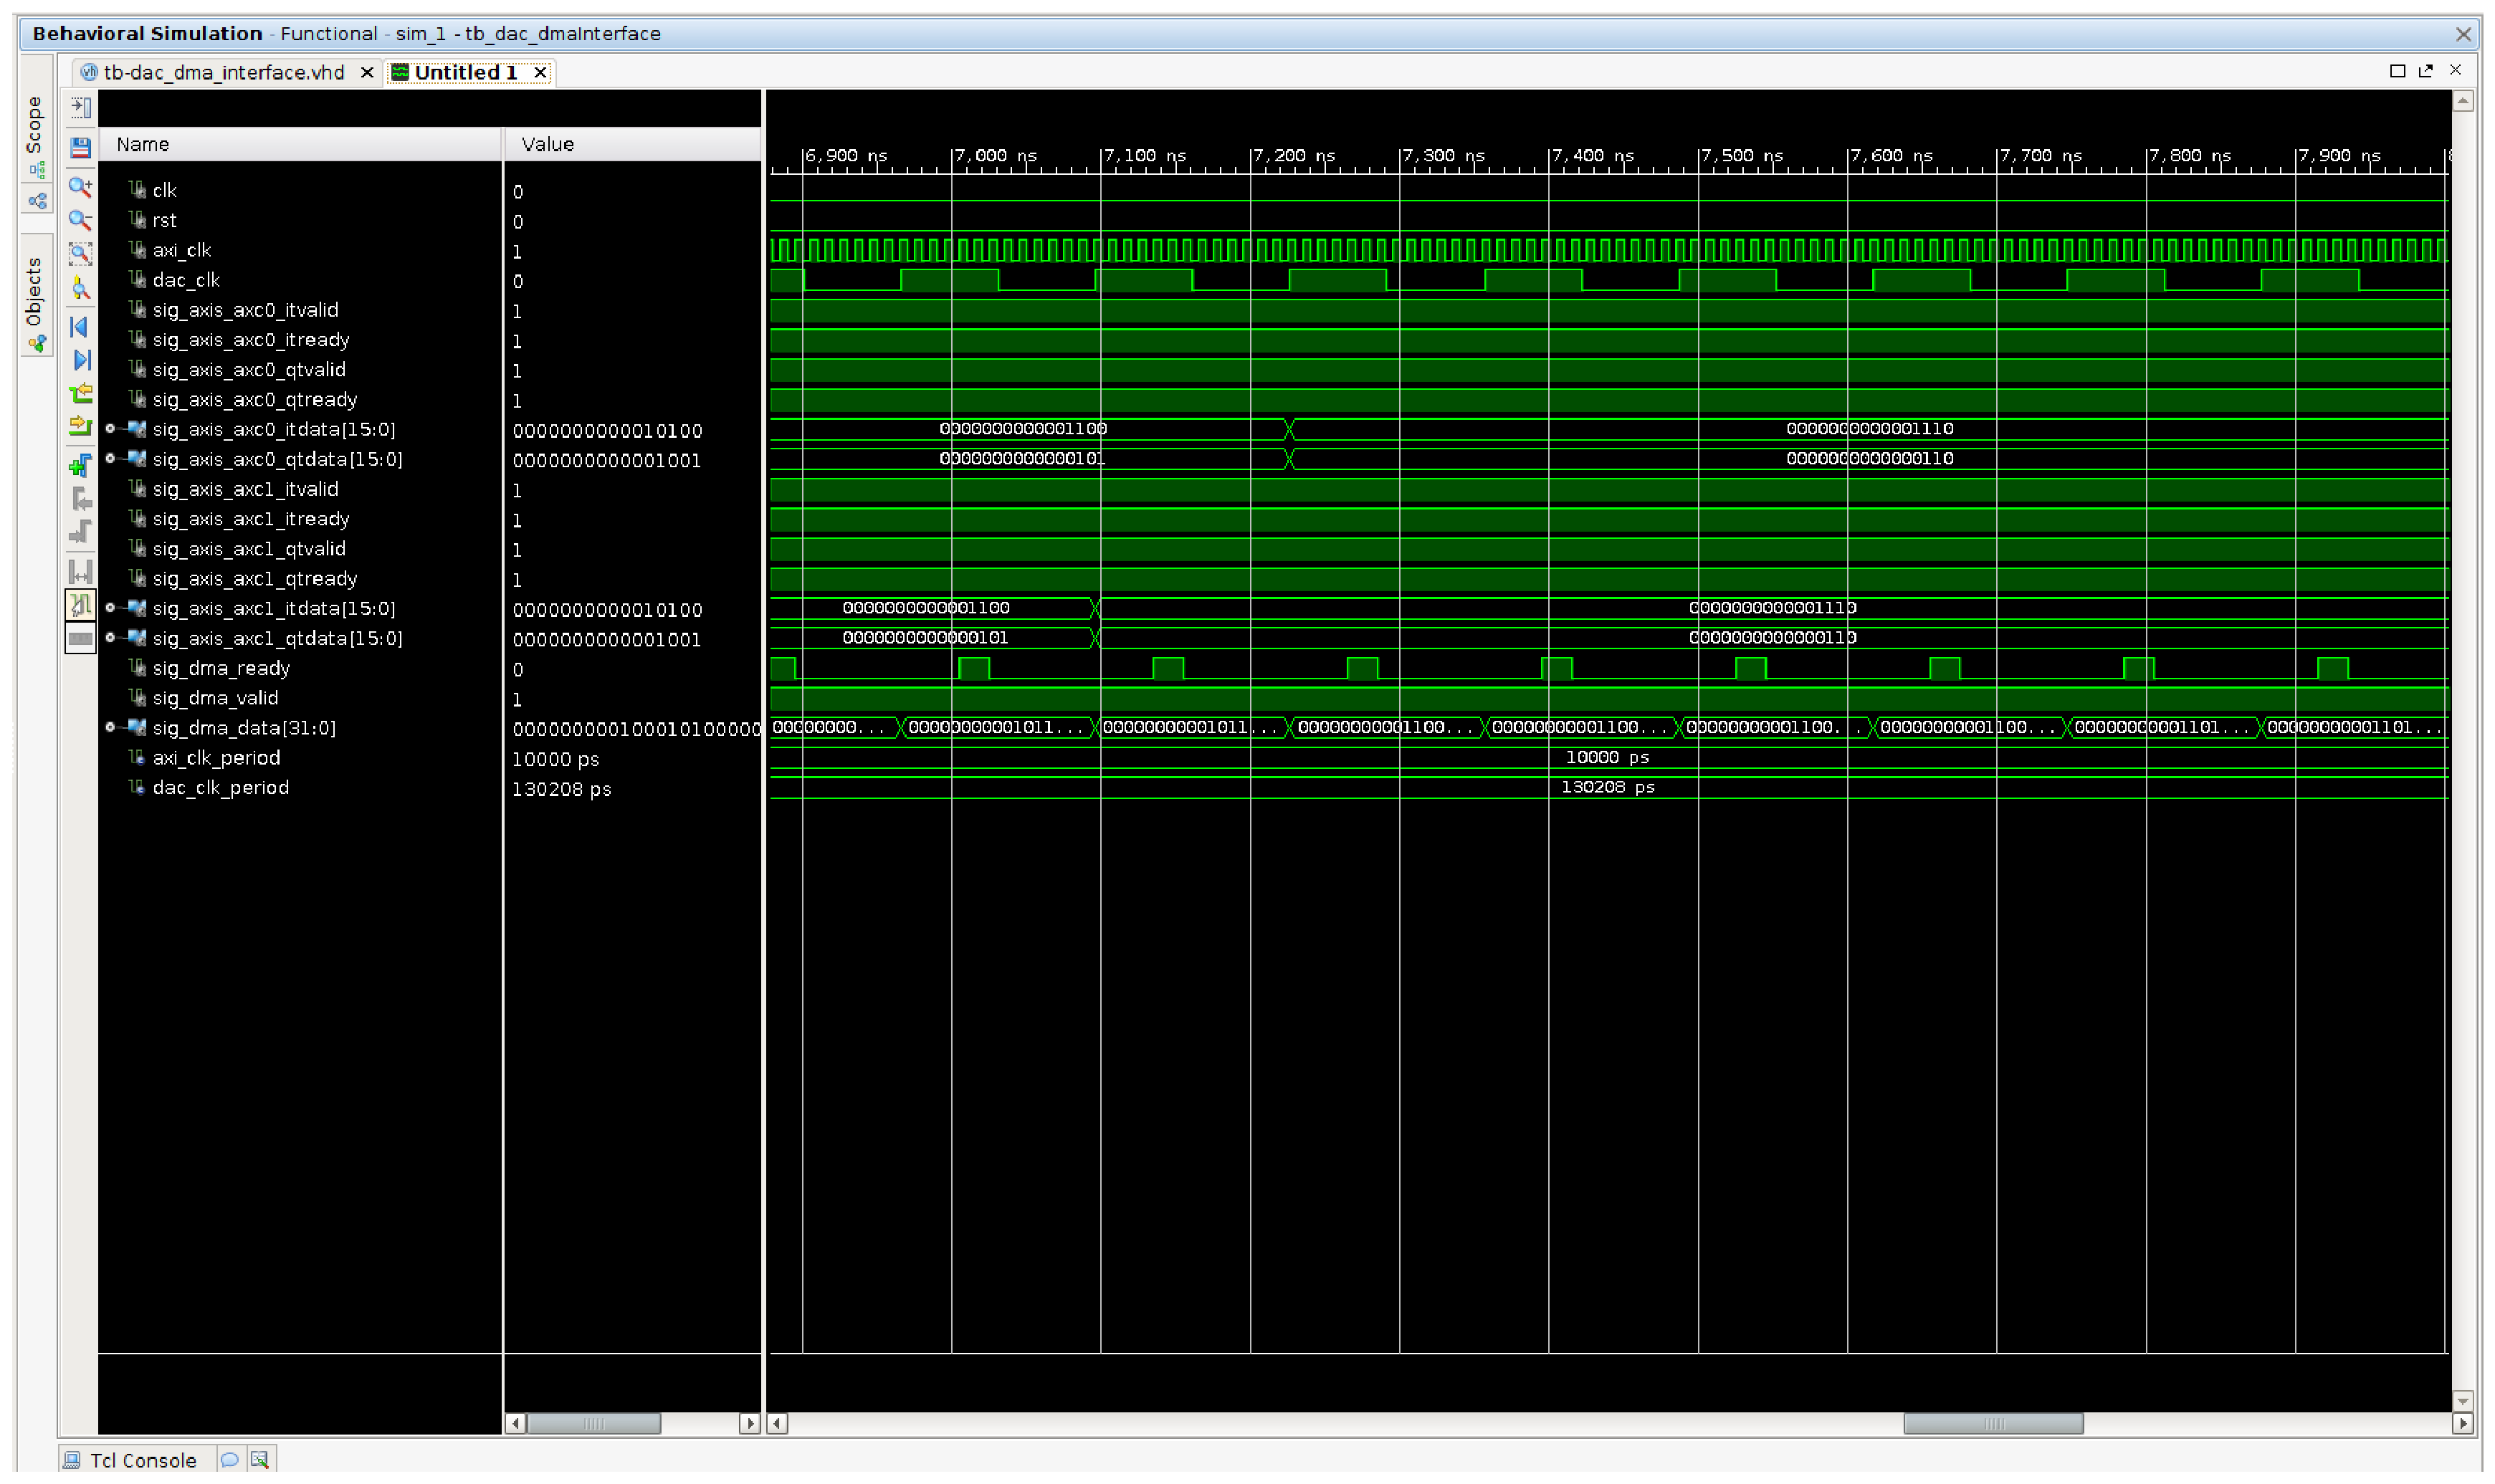
\includegraphics[width=0.95\textwidth]{./figures/dac_dmaInterface}
    \caption{ Step 1: DAC-DMA Interface Block Simulation
    \label{fig:simdacdma}}
\end{figure}

 In the figure \ref{fig:simdac} the \textit{dacInterface} is simulated and again
 it is possible to watch teh signals \textit{sig\_axis\_axc0\_itdata,
 sig\_axis\_axc0\_qtdata, sig\_axis\_axc1\_itdata and sig\_axis\_axc1\_qtdata} being fed
 to the block and the outputs \textit{sig\_dac\_i0data, sig\_dac\_q0data,
 sig\_dac\_i1data and sig\_dac\_q1data}, teh point in both \textit{dac-dmaIterface}
 and \textit{dacInterface} is to watch ghanges in outputs accompanying
 \textit{ready and valid} signals whcih are used as a way of controlling reading
 speed from the \textit{DMA}, in such scheme, the \textit{DMA} assets
 \textit{valid} whenever is can send data, however it only send teh data when
 fed by a ready signal, meaning that the reading block can read the \textit{DMA}
 data.

\begin{figure}[htbp]
    \centering
    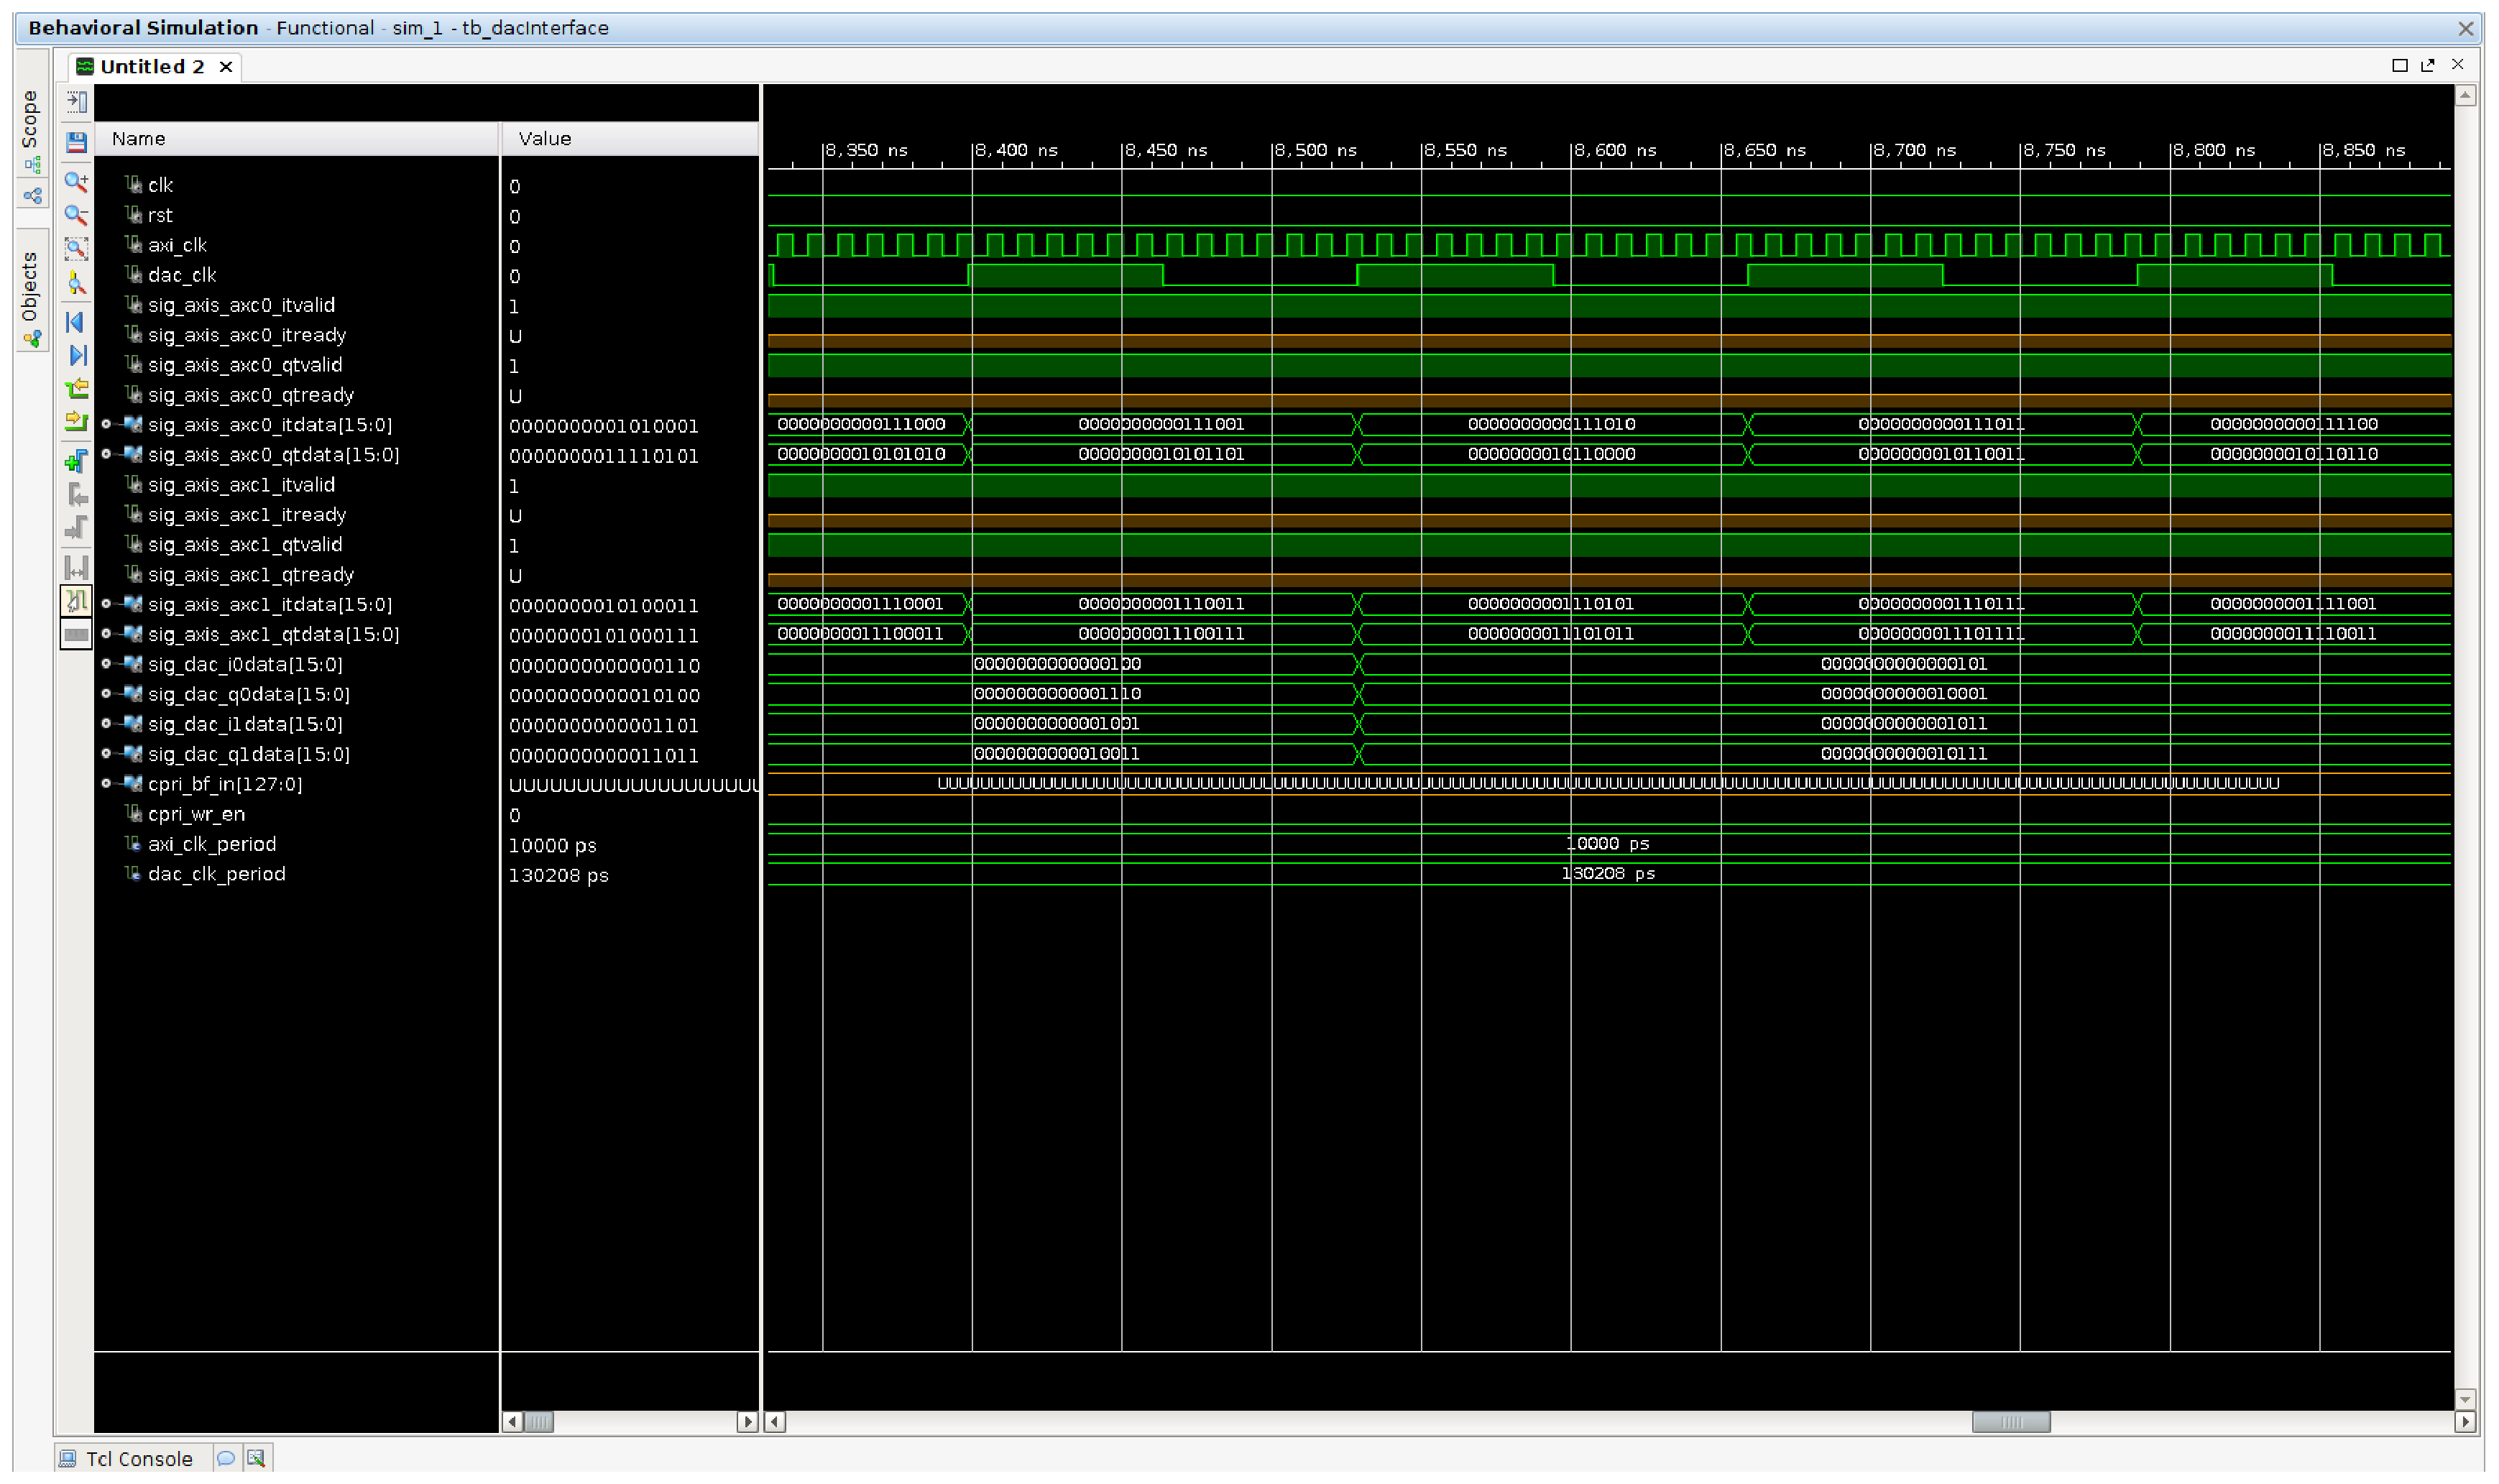
\includegraphics[width=0.95\textwidth]{./figures/dacInterface}
    \caption{ Step 2: DAC Interface Block Simulation
    \label{fig:simdac}}
\end{figure}

In the final simulation of the transmitting interface the whole transmit chain
blocks were simulated toghether and then is is possible to understand the
behavior of the whole transmit interface block. In the figure \ref{fig:simtxif}
it is possible to watch the \textit{DMA} data in the signal in
\textit{dac-dmaIterface} and the outputs which woul fedd the \textit{AD9361}
two \textit{DACs} in the signals \textit{sig\_dac\_i0data, sig\_dac\_q0data,
sig\_dac\_i1data and sig\_dac\_q1data}, again the important thing in the simulation
is to watch for the data change and the  \textit{ready and valid} changes.
Another interesting thing to observ is the two clock variables \textit{axi\_clk}
and \textit{dac\_clk} which represent both axi system clock $ 100 MHz$ and the
dac clock $40 MHz$, this difference justifies the use of such interface.


\begin{figure}[htbp]
    \centering
    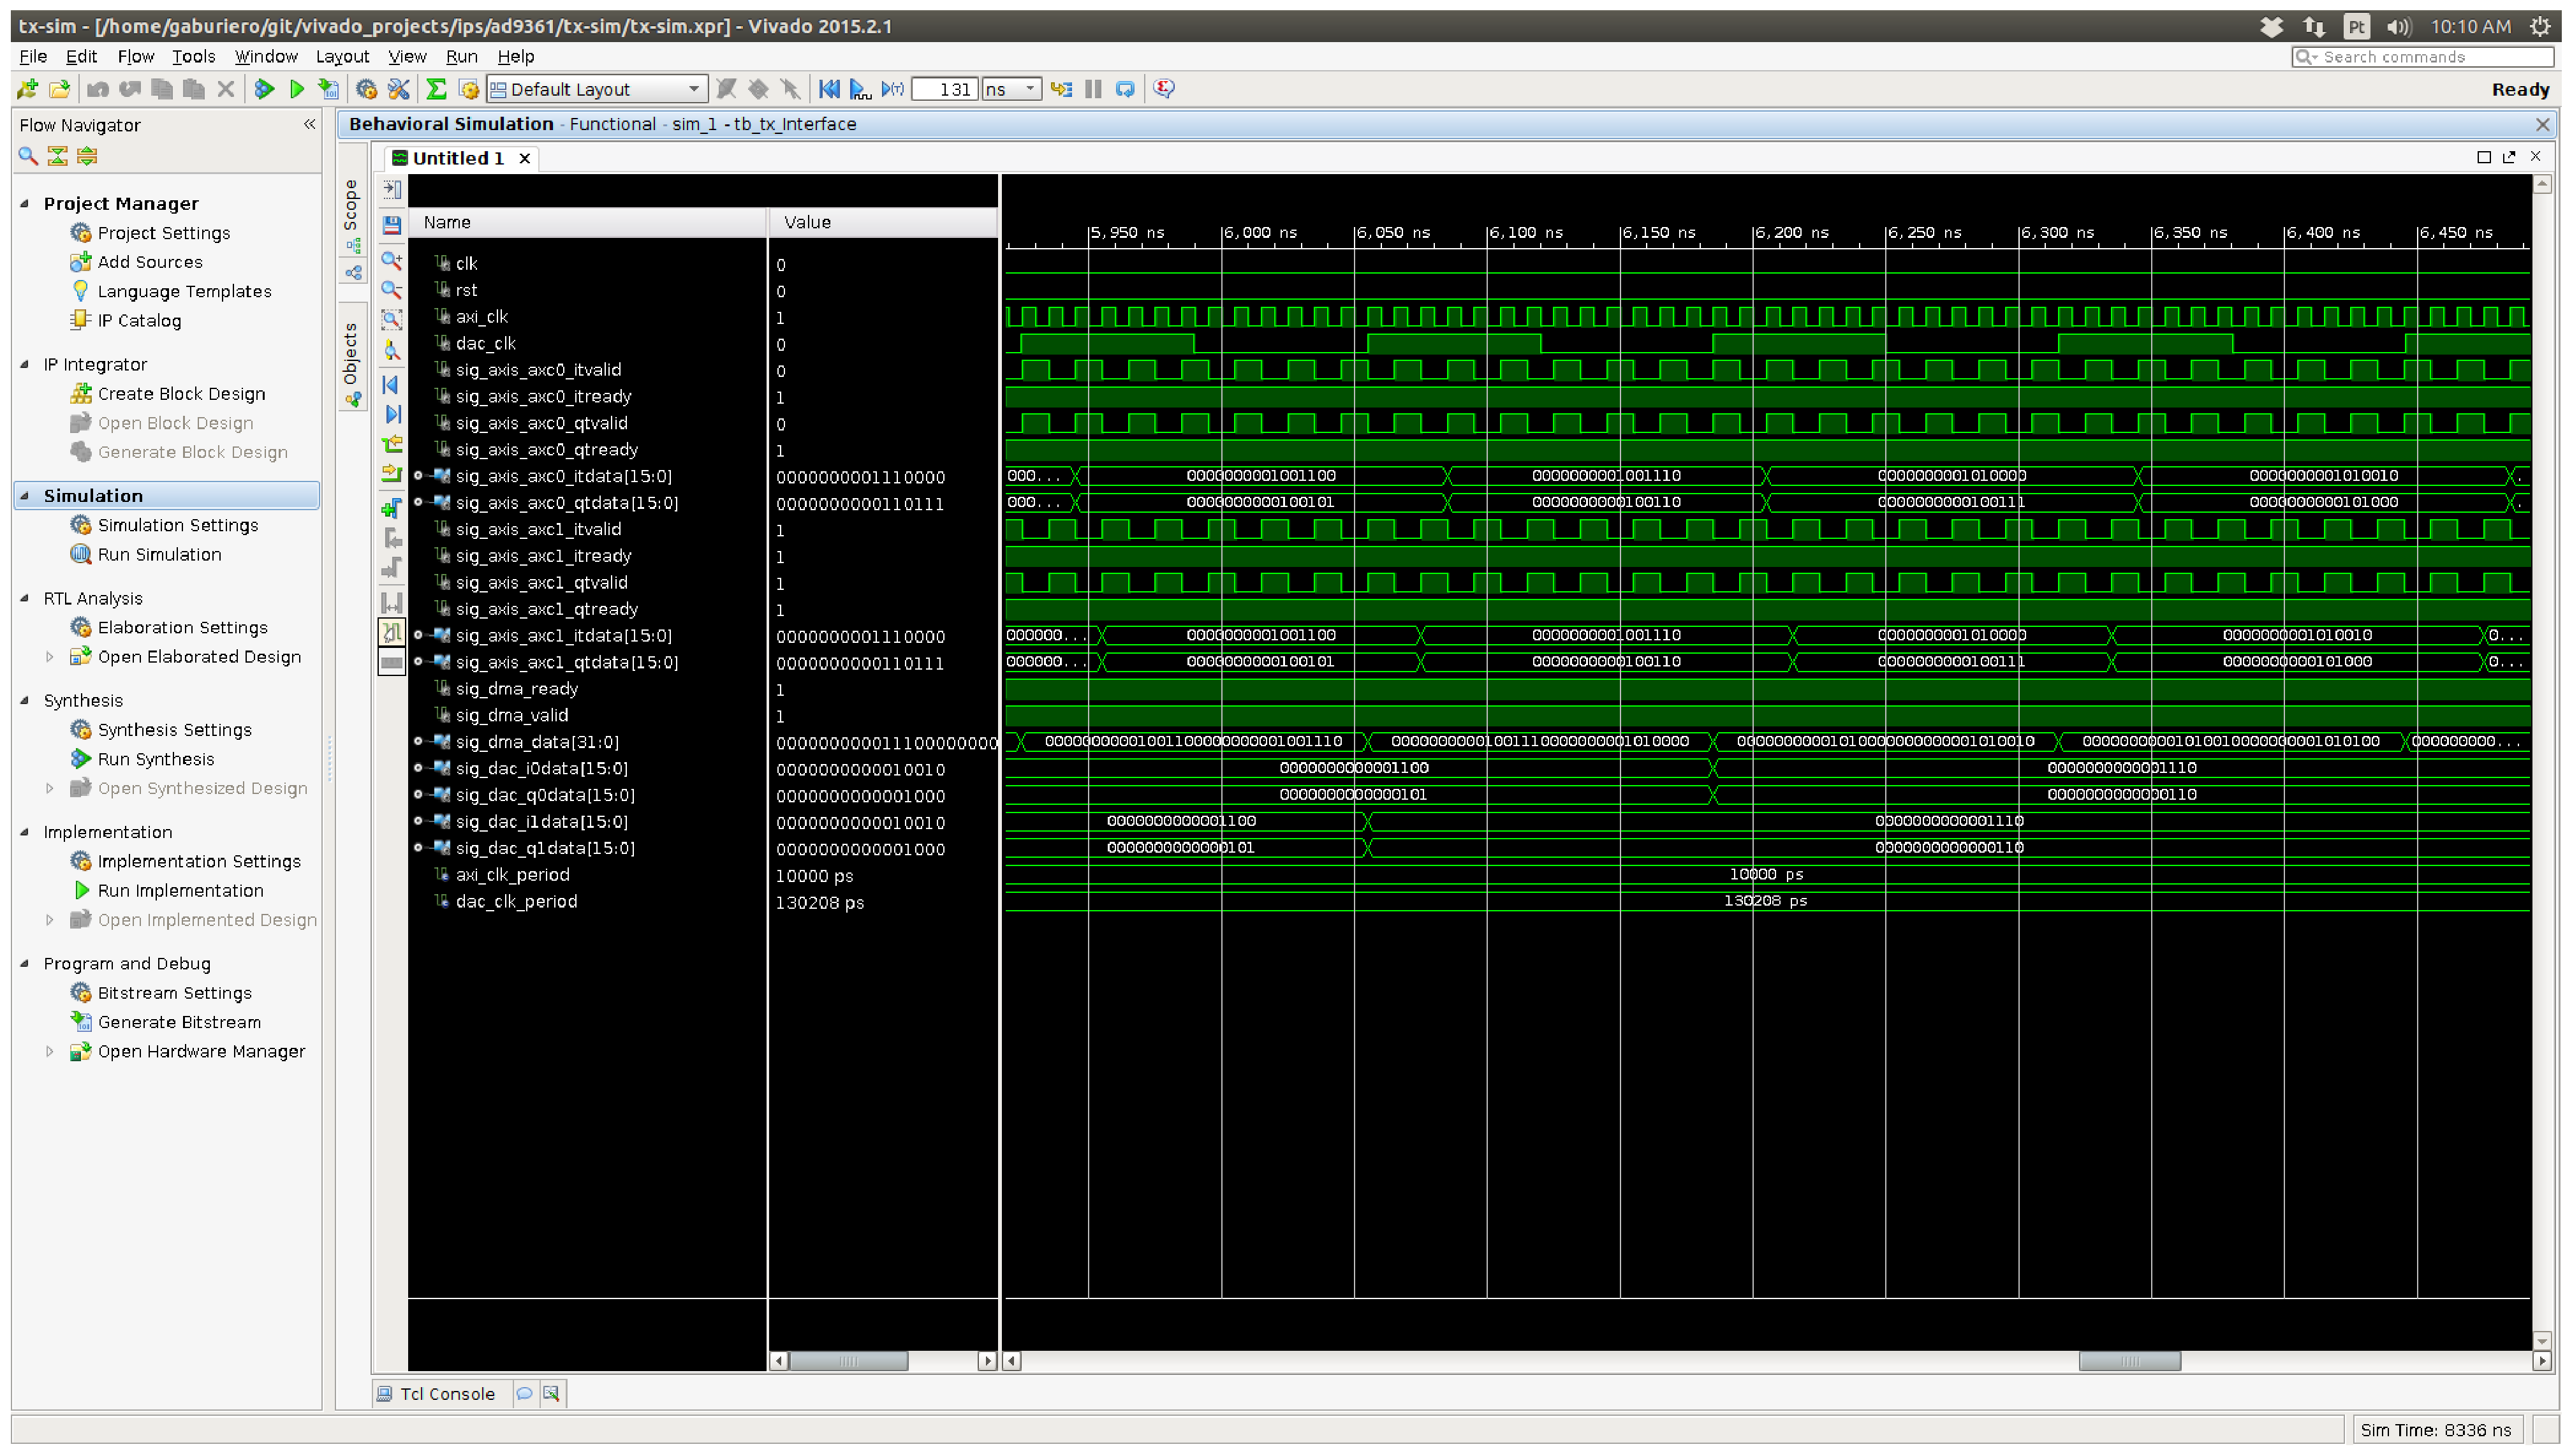
\includegraphics[width=0.95\textwidth]{./figures/txInterface}
    \caption{ Step 3: Transmitting Interface Block Simulation
    \label{fig:simtxif}}
\end{figure}

\subsection{Receive (ADC) Interface Simulation}

As stated before on chapter \ref{chap:implementation} in the section \ref{impl:setup},
the DAC interface is simple beacause the data input is already limited by the DAC
clock, so there is no need to make a bottleneck like in the DAC interface.

 In the figure \ref{fig:simdac} it is possible to see the output and wave
diagram in the simulation window. Since the \textit{adcInterface} is much more
simpler, because the data input is already limited by the \textit{AD9361}
clock, in the signals \textit{sig\_rx\_i0\_data, sig\_rx\_q0\_data,
sig\_rx\_i1\_data, sig\_rx\_q1\_data} there is the outputs from both
\textit{DACs} and \textit{dout} is the data that will be fed to the
\textit{DMA}.\\

\begin{figure}[htbp]
    \centering
    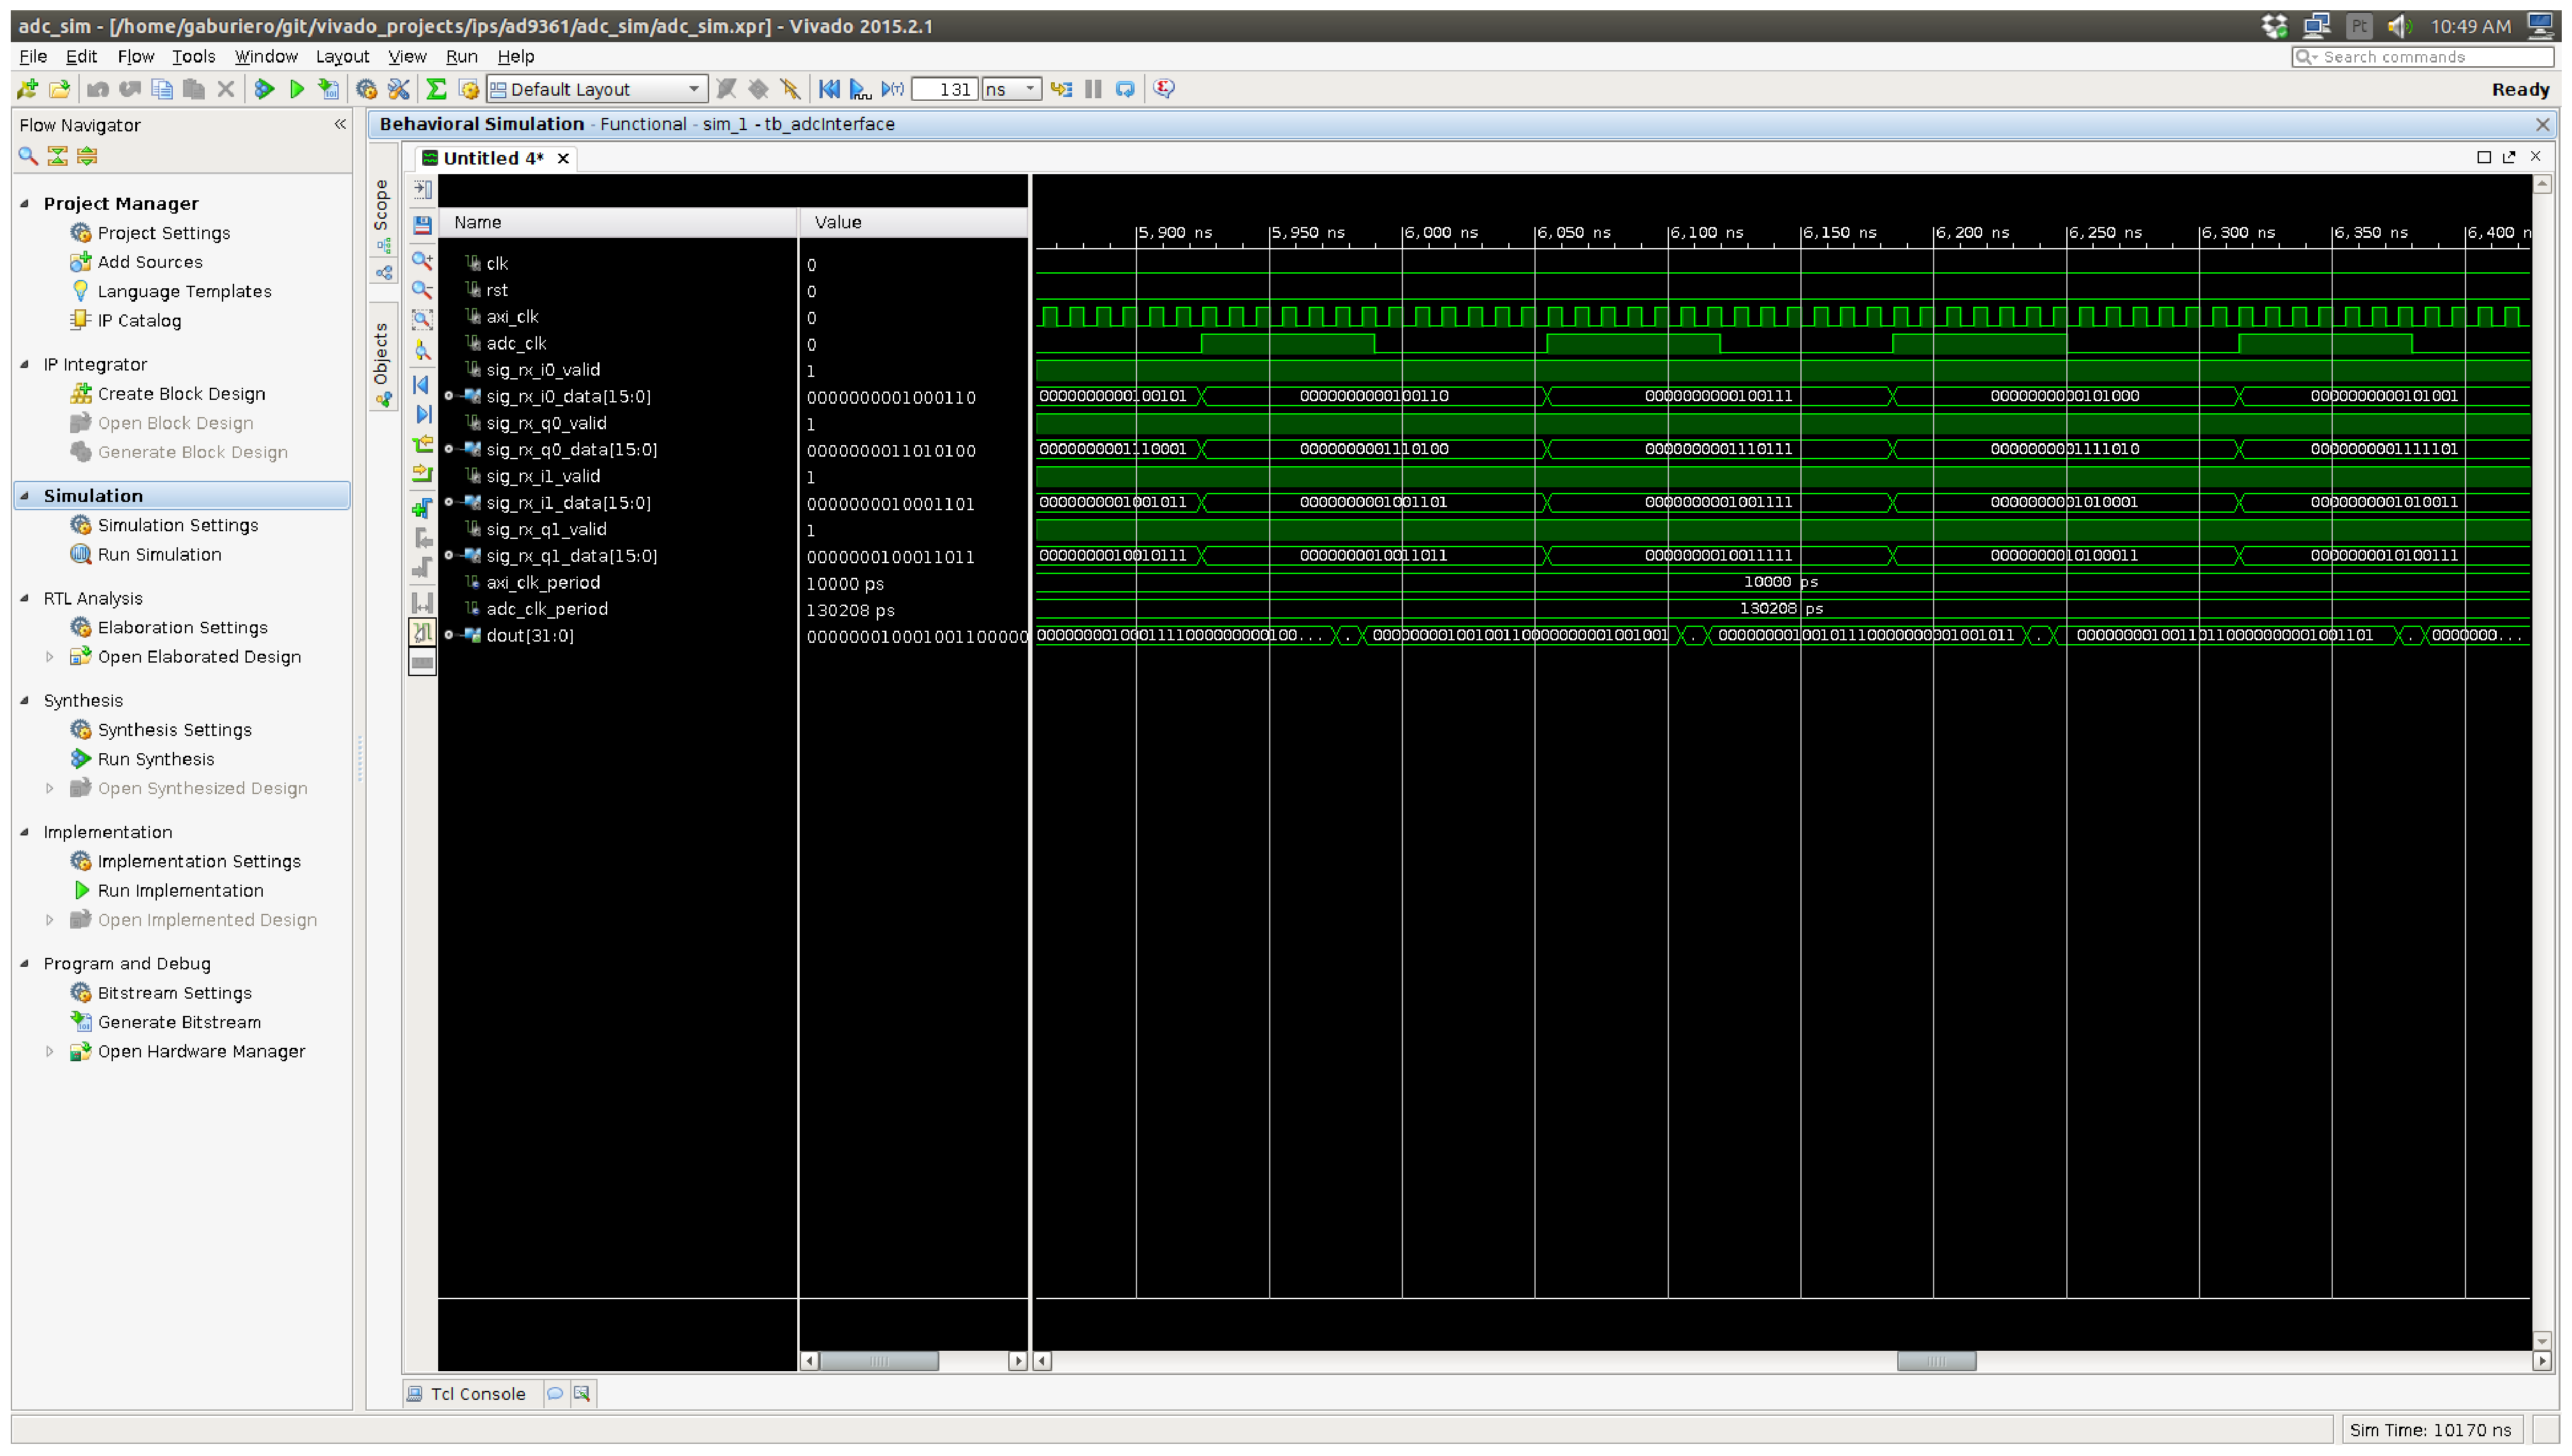
\includegraphics[width=0.95\textwidth]{./figures/adcInterface}
    \caption{ ADC Interface Block Simulation
    \label{fig:simadc}}
\end{figure}

\vfill
\clearpage

\section{Transmission Tests (DAC)}
\label{result:dac}

 The transmission tests aim to evaluate a Donwlink LTE transmission, it means
that the data is being transmitted from the BTS to the UE. In this trnasmission
test there were generated LTE samples in matlab, and these samples were loaded
in the memory by putting them in a header file, the as explained before, DMA
shall read them and the DAC shall make an analog output. In the figure
\ref{fig:dacsignals} there are the DAC control signals sent to the data
interface block in order to control the data flow, thus this control makes a
back-pressure in the DMA engine controlling if DMA reads or not data from
memory, thus the DMA Engine reading output can be seen in the figures
\ref{fig:dataflowdig} and \ref{fig:dataflowana}, digital and analog waveforms
respectively.\\

 It is possible to configure in the driver if the AD9361 ouputs or not a clock
in a special clock\_output pin, so in order to evaluate frequency and clock
quality, the figure \ref{fig:dacclk} shows the clock output from the AD9361 and
last but not least the figure \ref{fig:lte5m} show the output spectrum of the
LTE analog wave outputted from the FMComms2 board.

\begin{figure}[htbp]
    \centering
    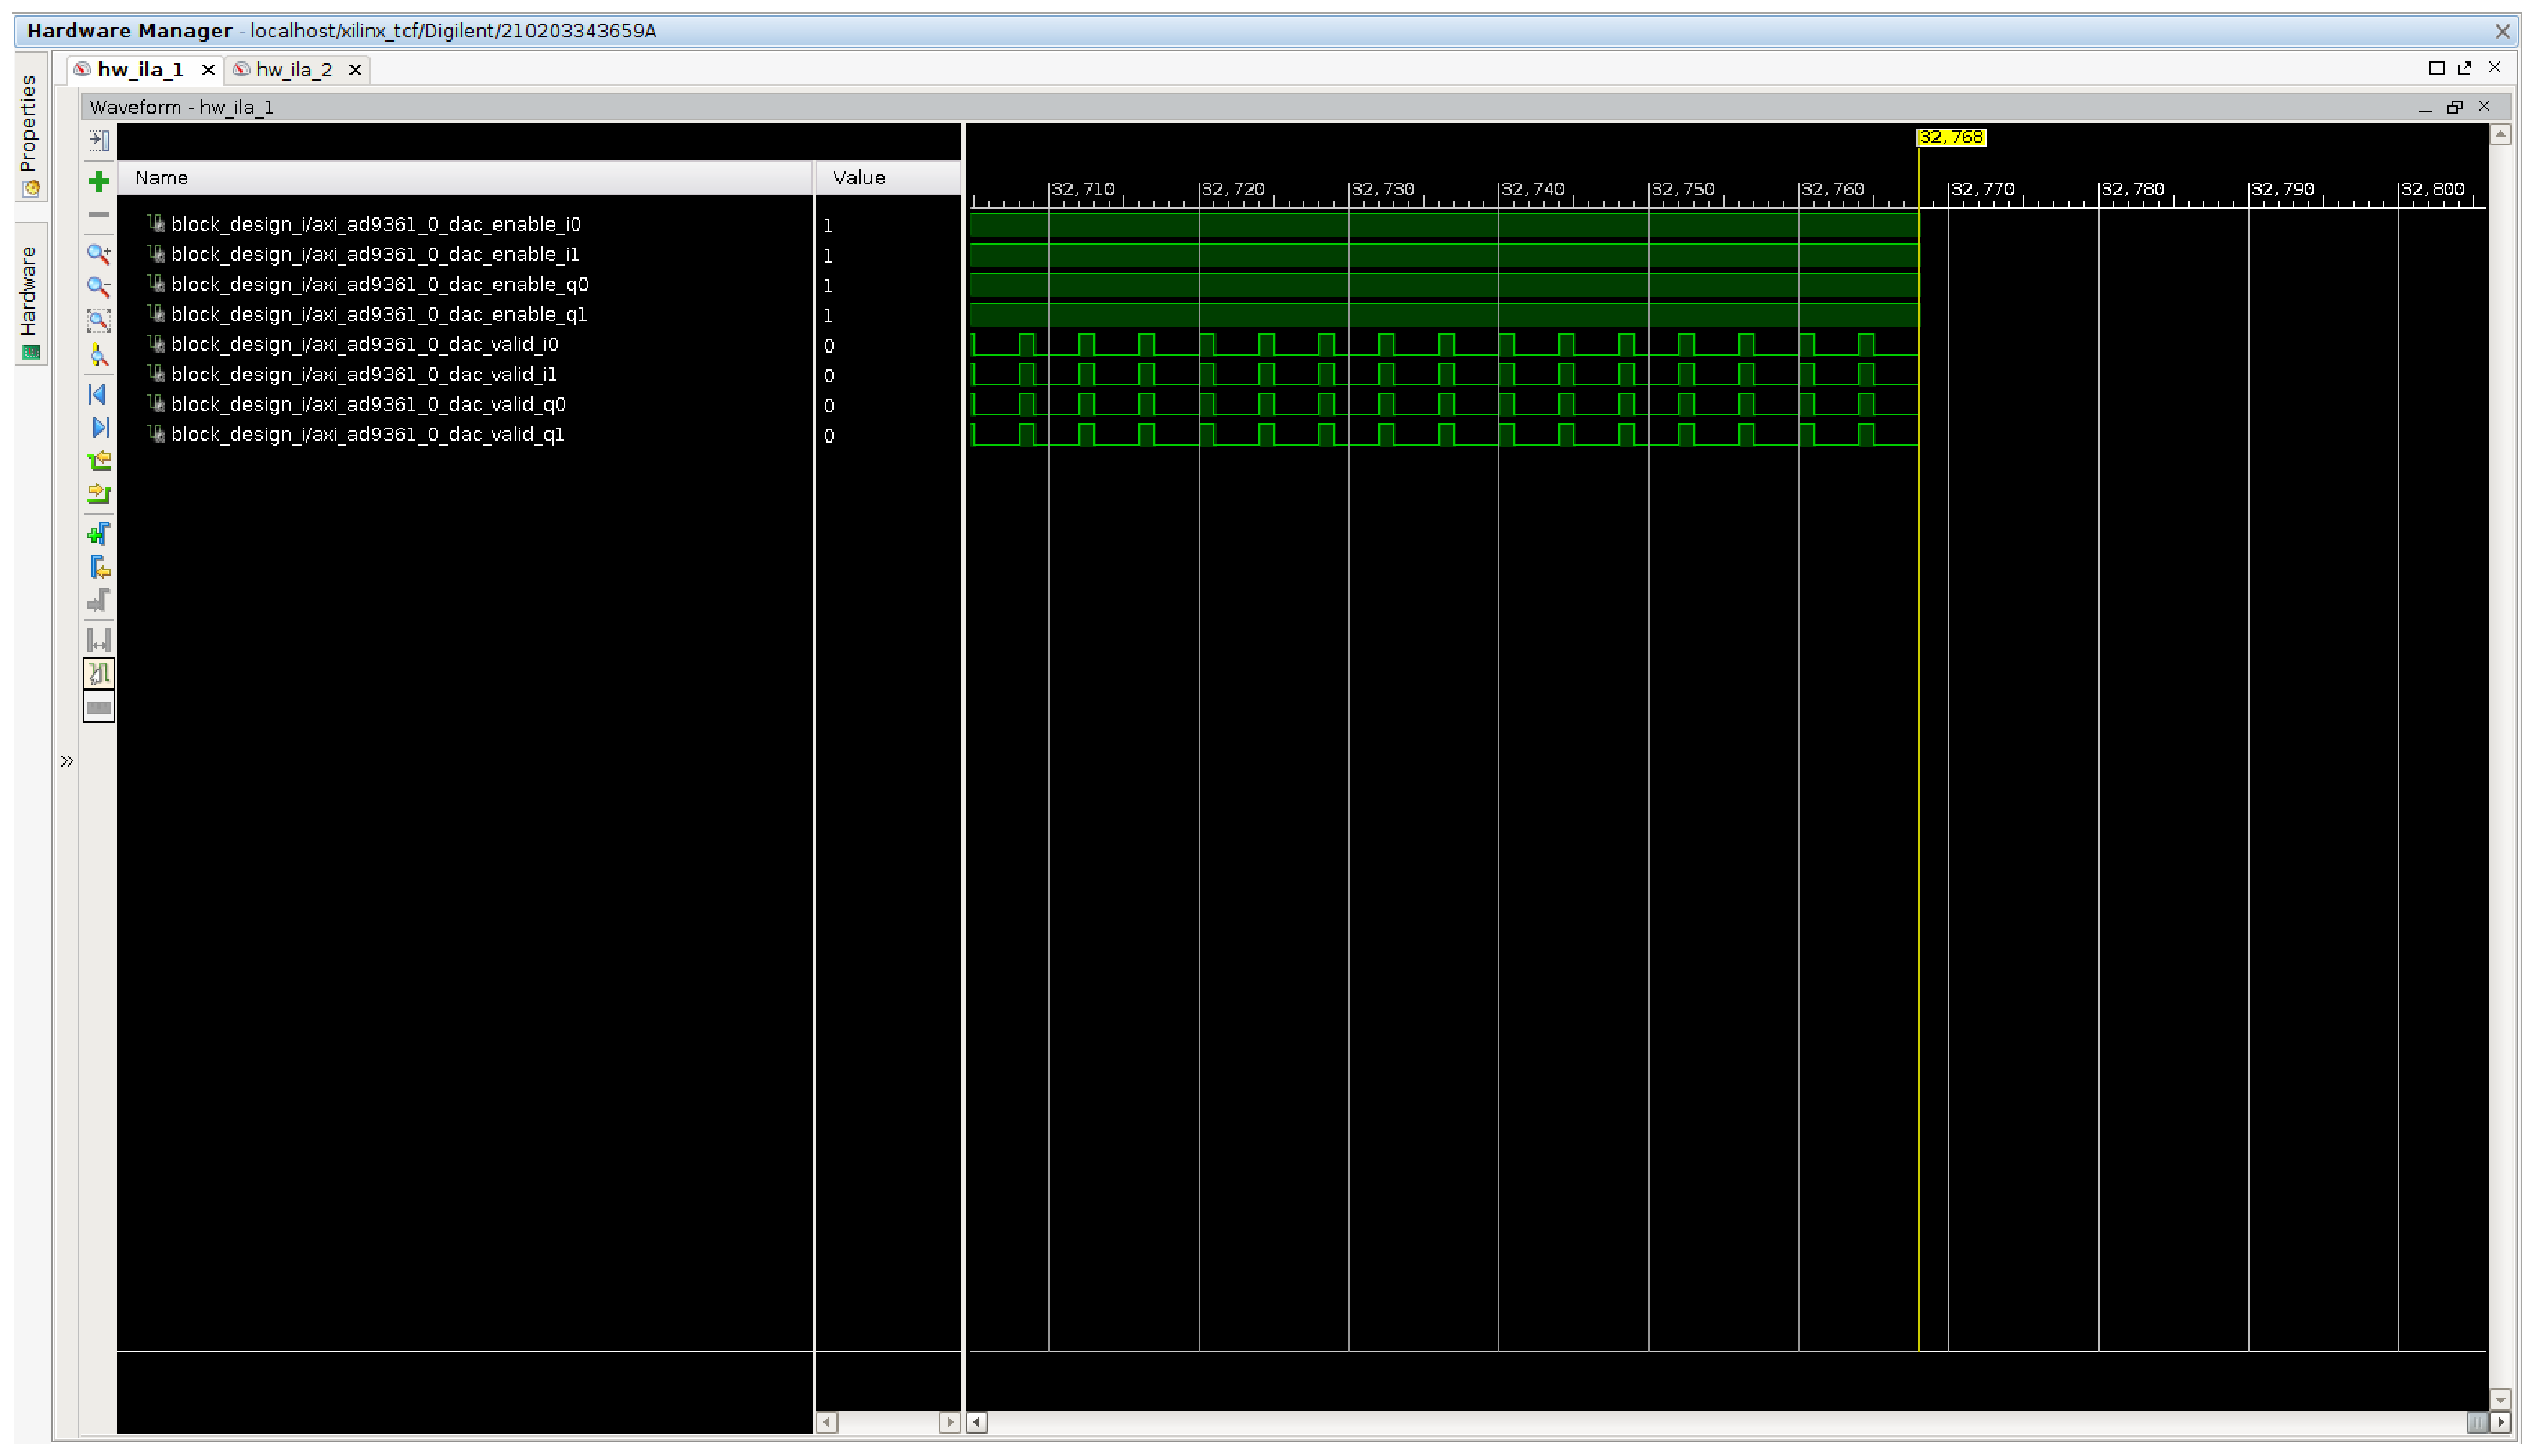
\includegraphics[width=0.85\textwidth]{./figures/dac_signals}
    \caption{ DAC signals controlling data reading
    \label{fig:dacsignals}}
\end{figure}

\begin{figure}[htbp]
    \centering
    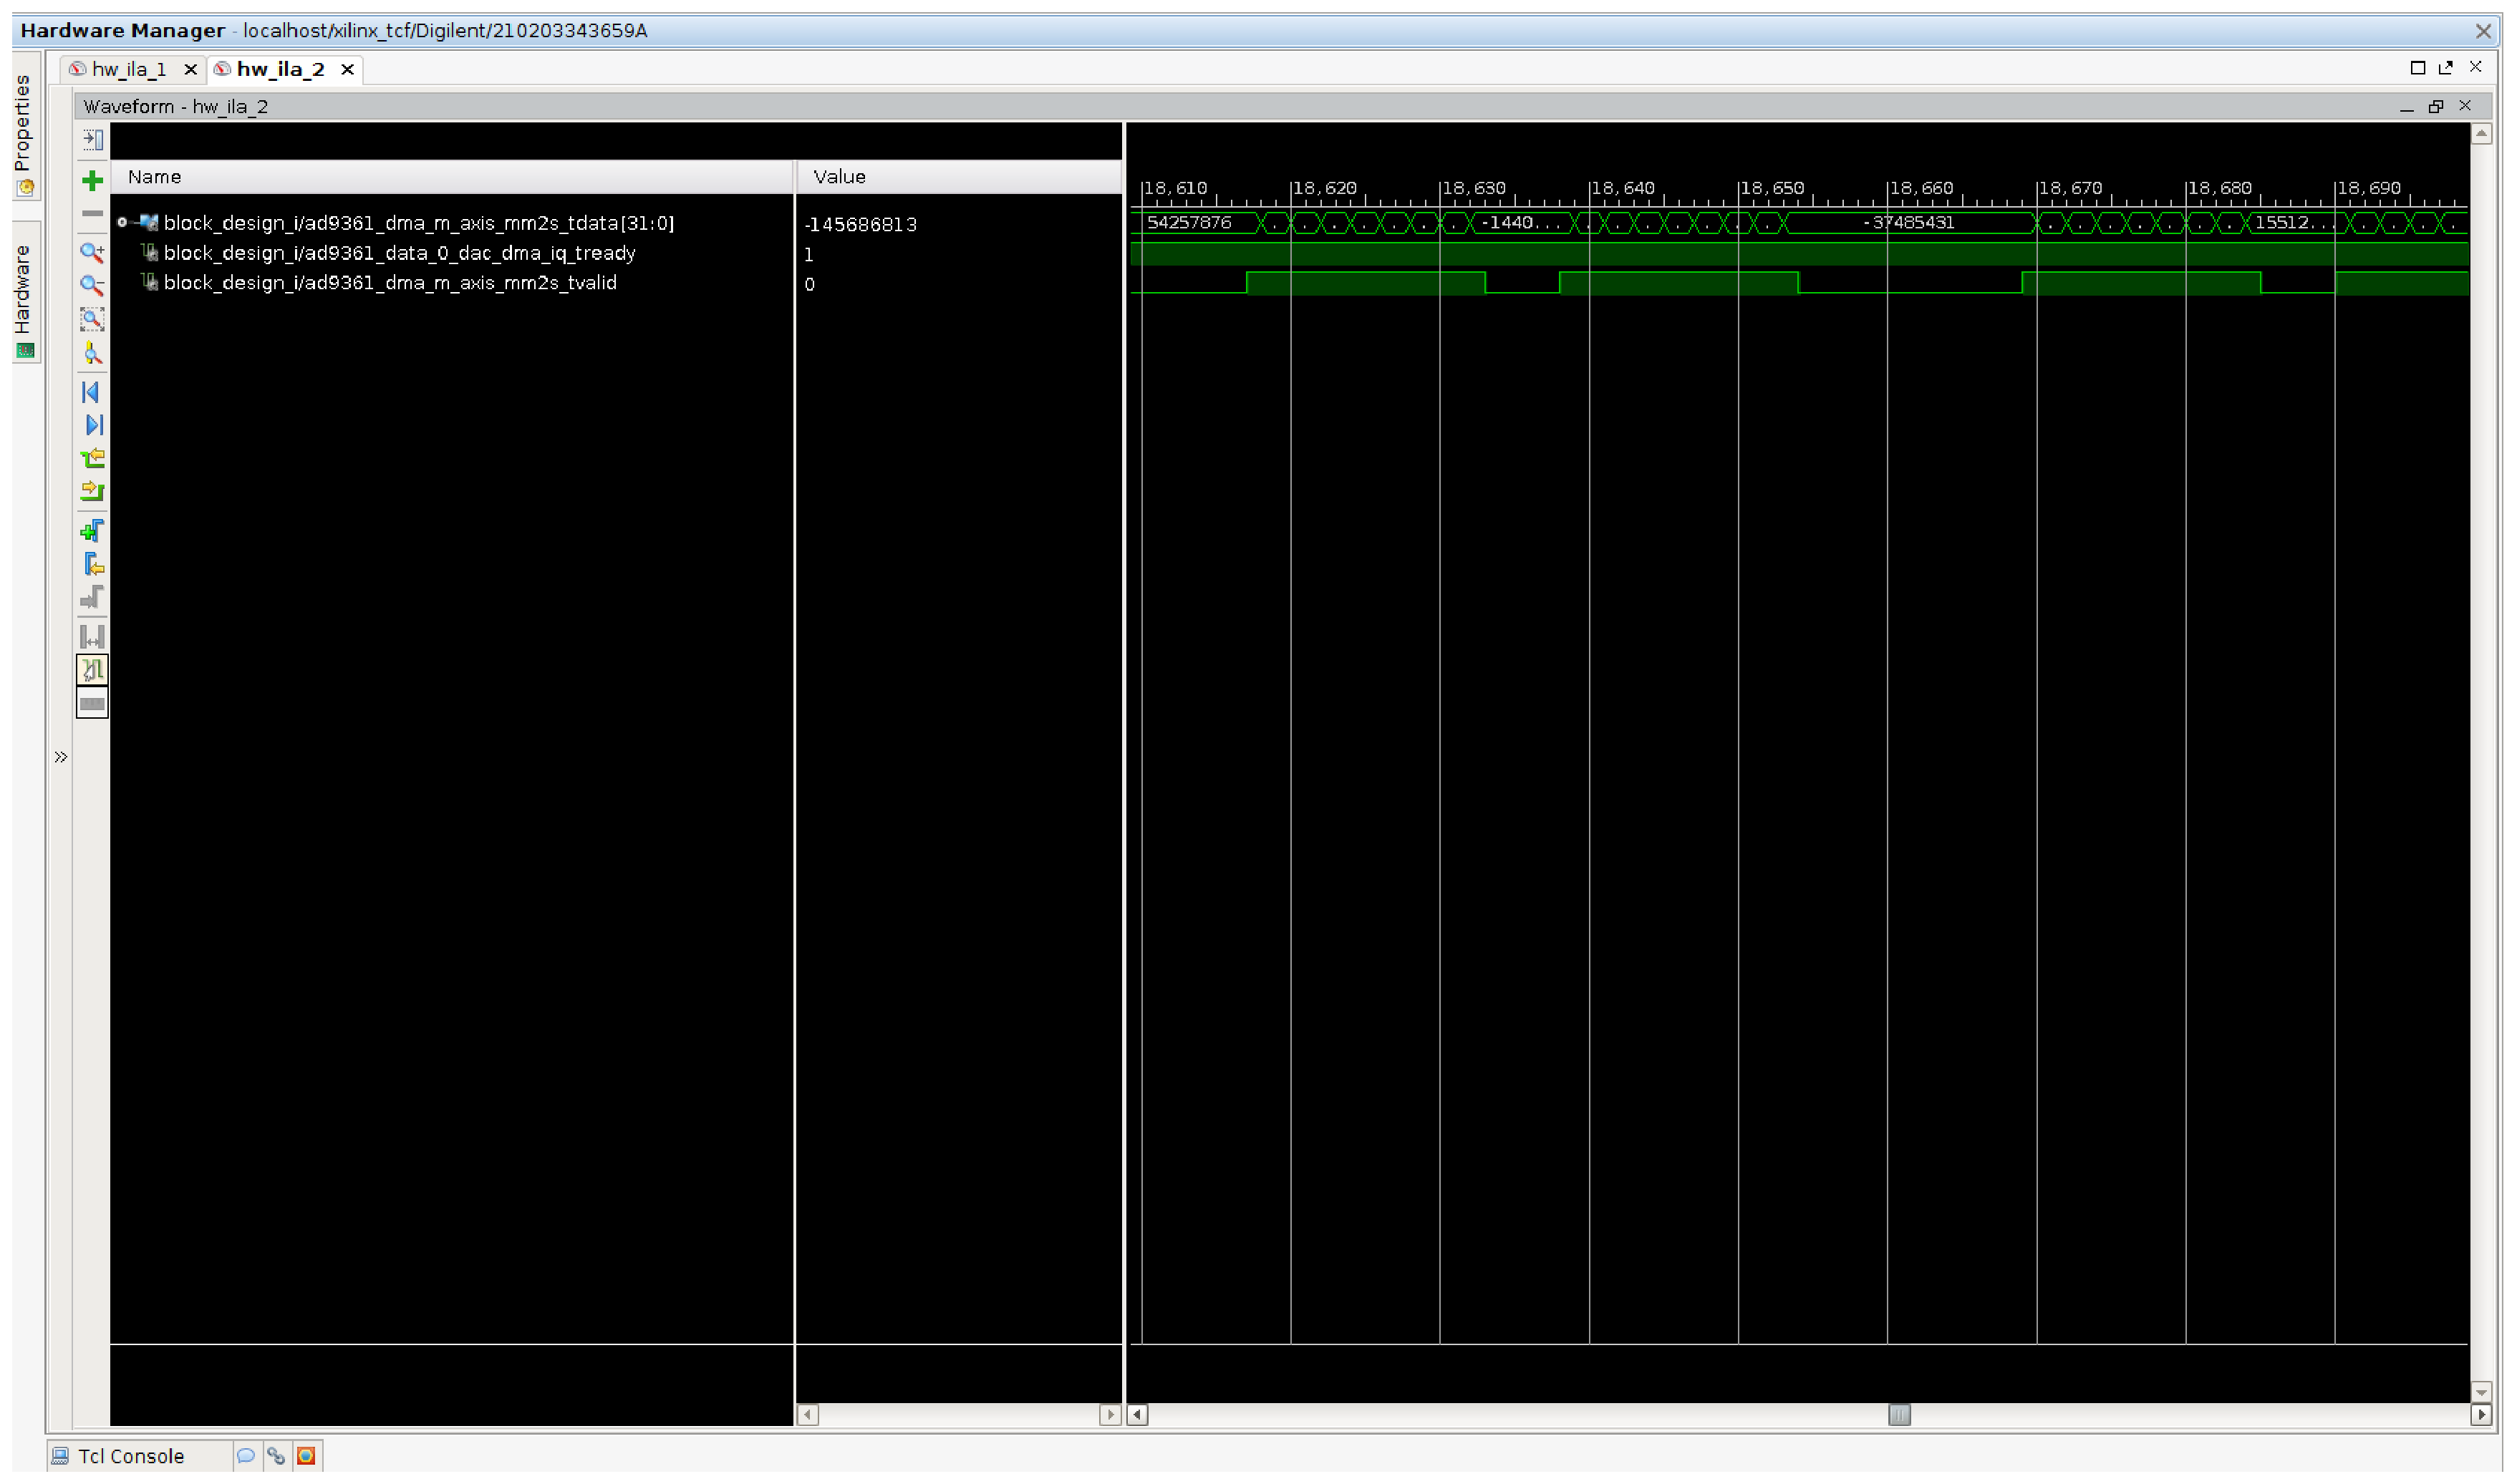
\includegraphics[width=0.85\textwidth]{./figures/ila_dataflow}
    \caption{ Digital Data read from memory by DMA.
    \label{fig:dataflowdig}}
\end{figure}

\begin{figure}[htbp]
    \centering
    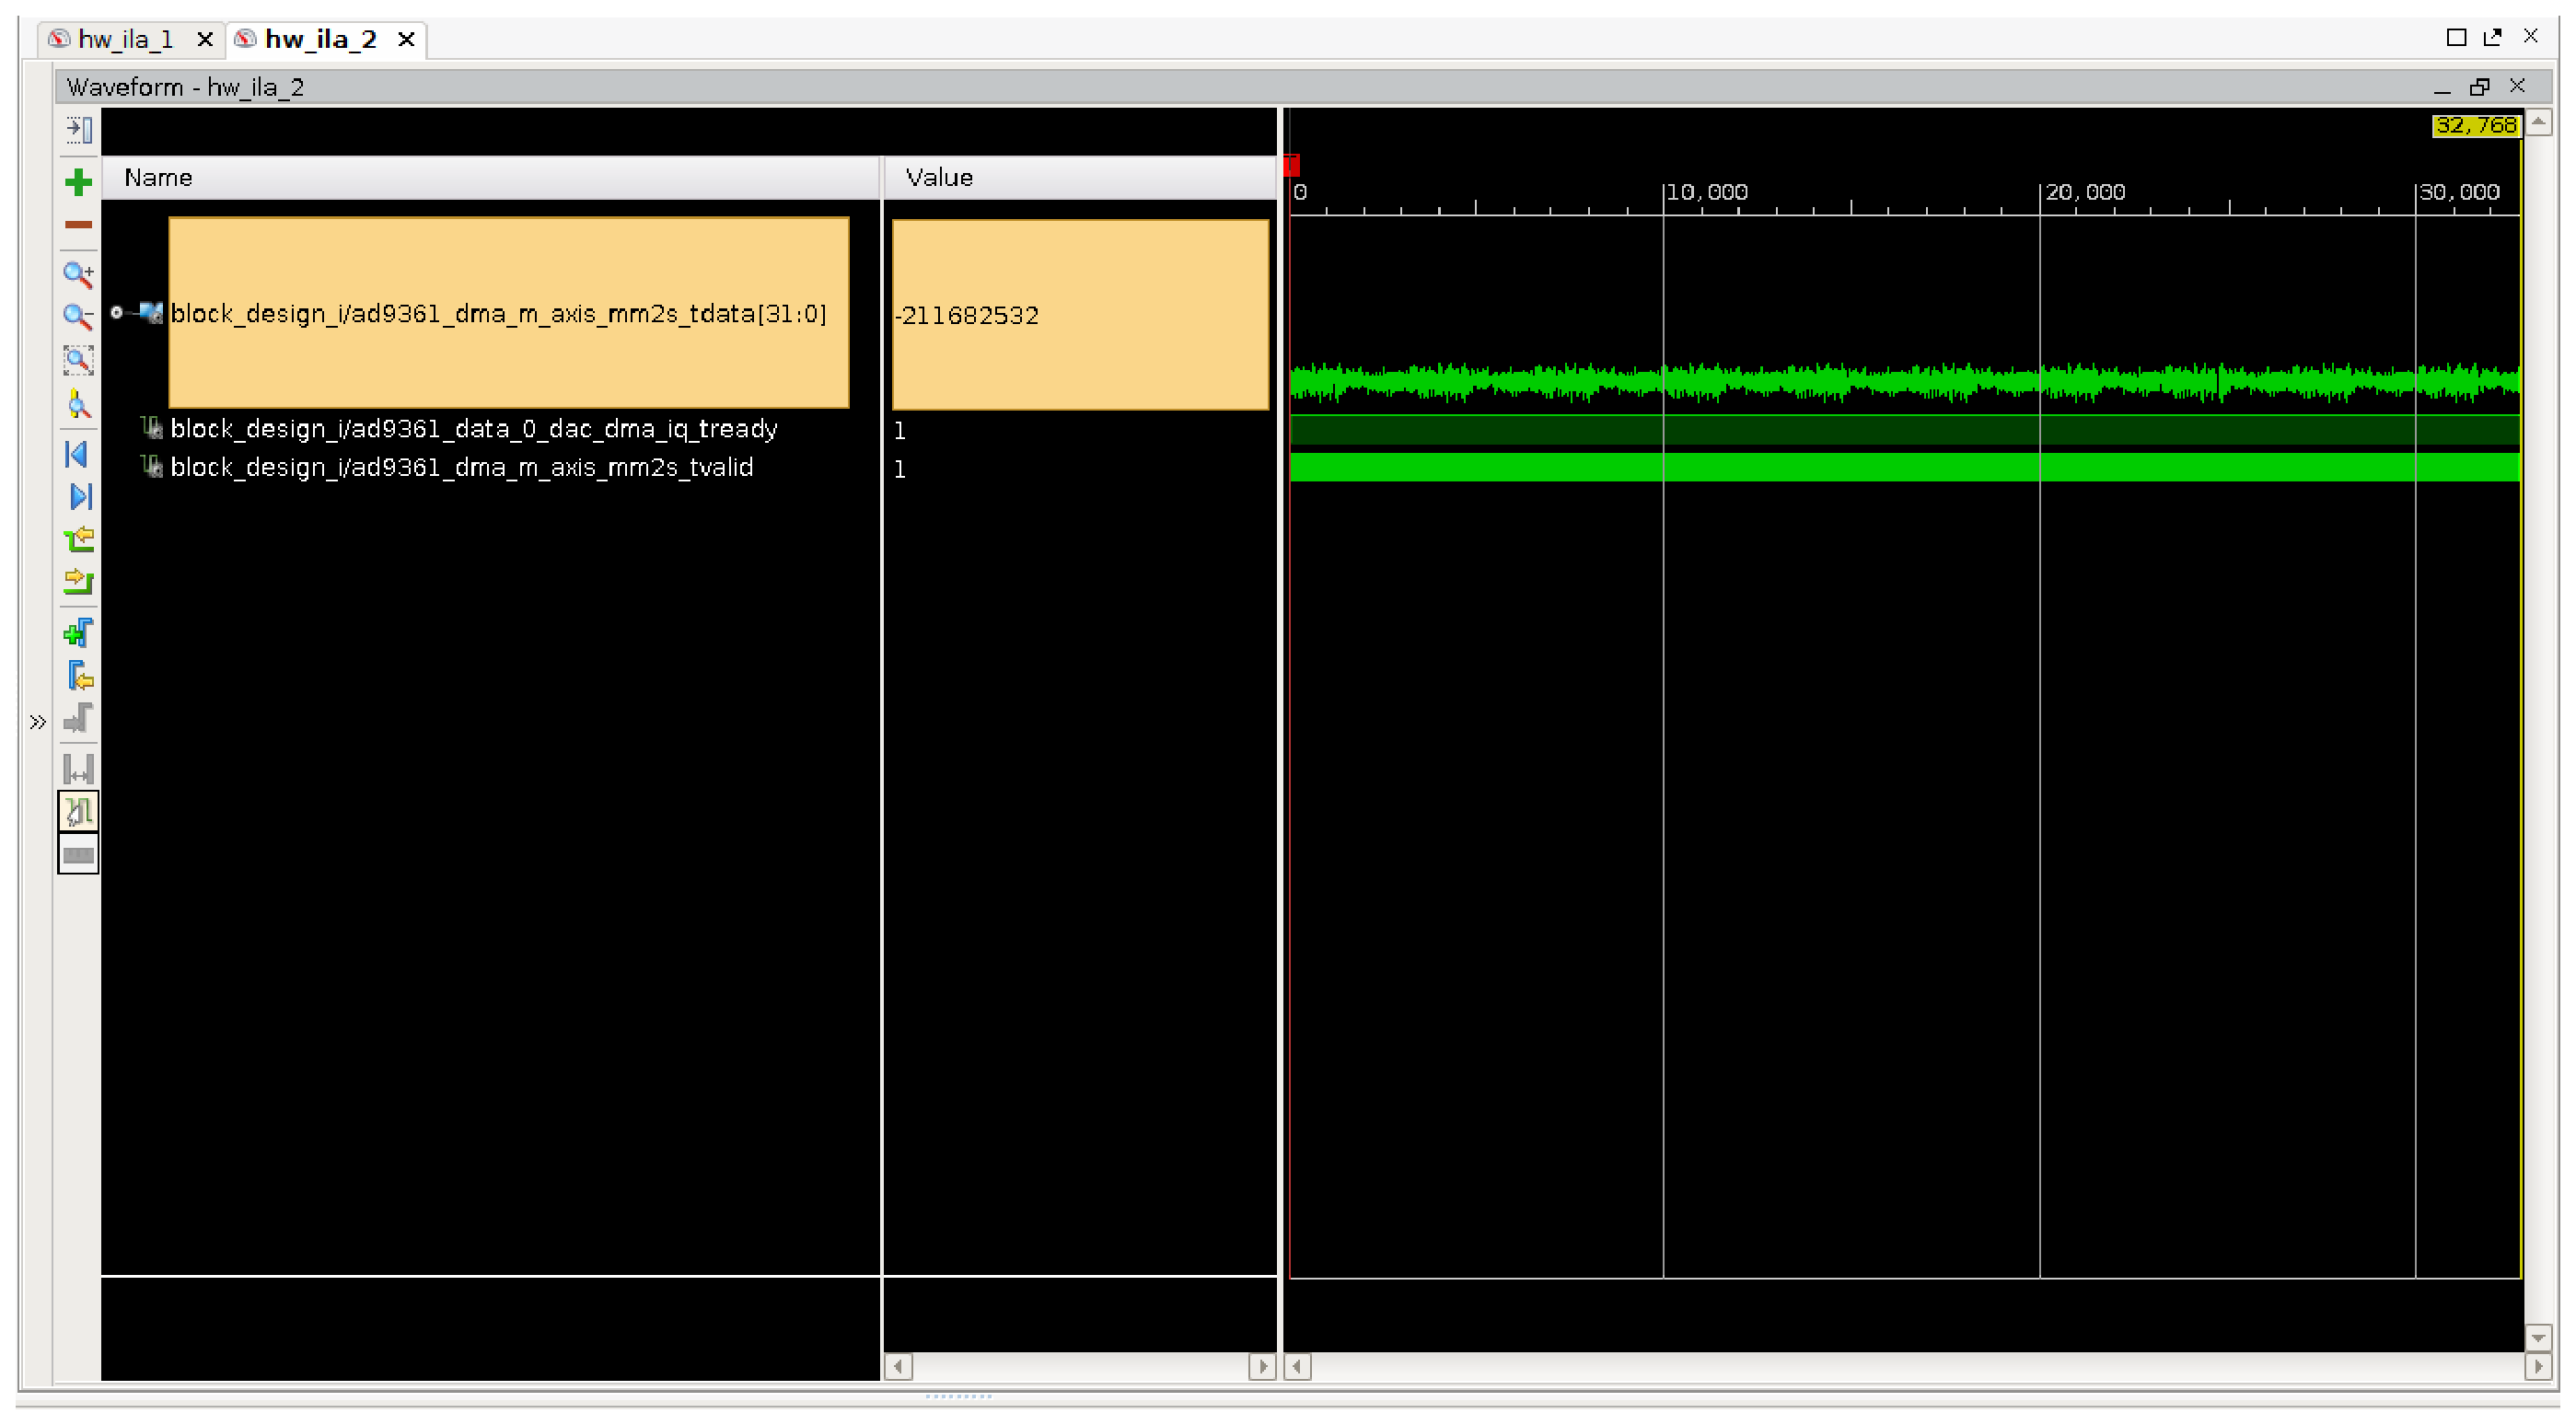
\includegraphics[width=0.85\textwidth]{./figures/ltedac_ila}
    \caption{ Analog form Data read form memory by DMA.
    \label{fig:dataflowana}}
\end{figure}

\begin{figure}[htbp]
    \centering
    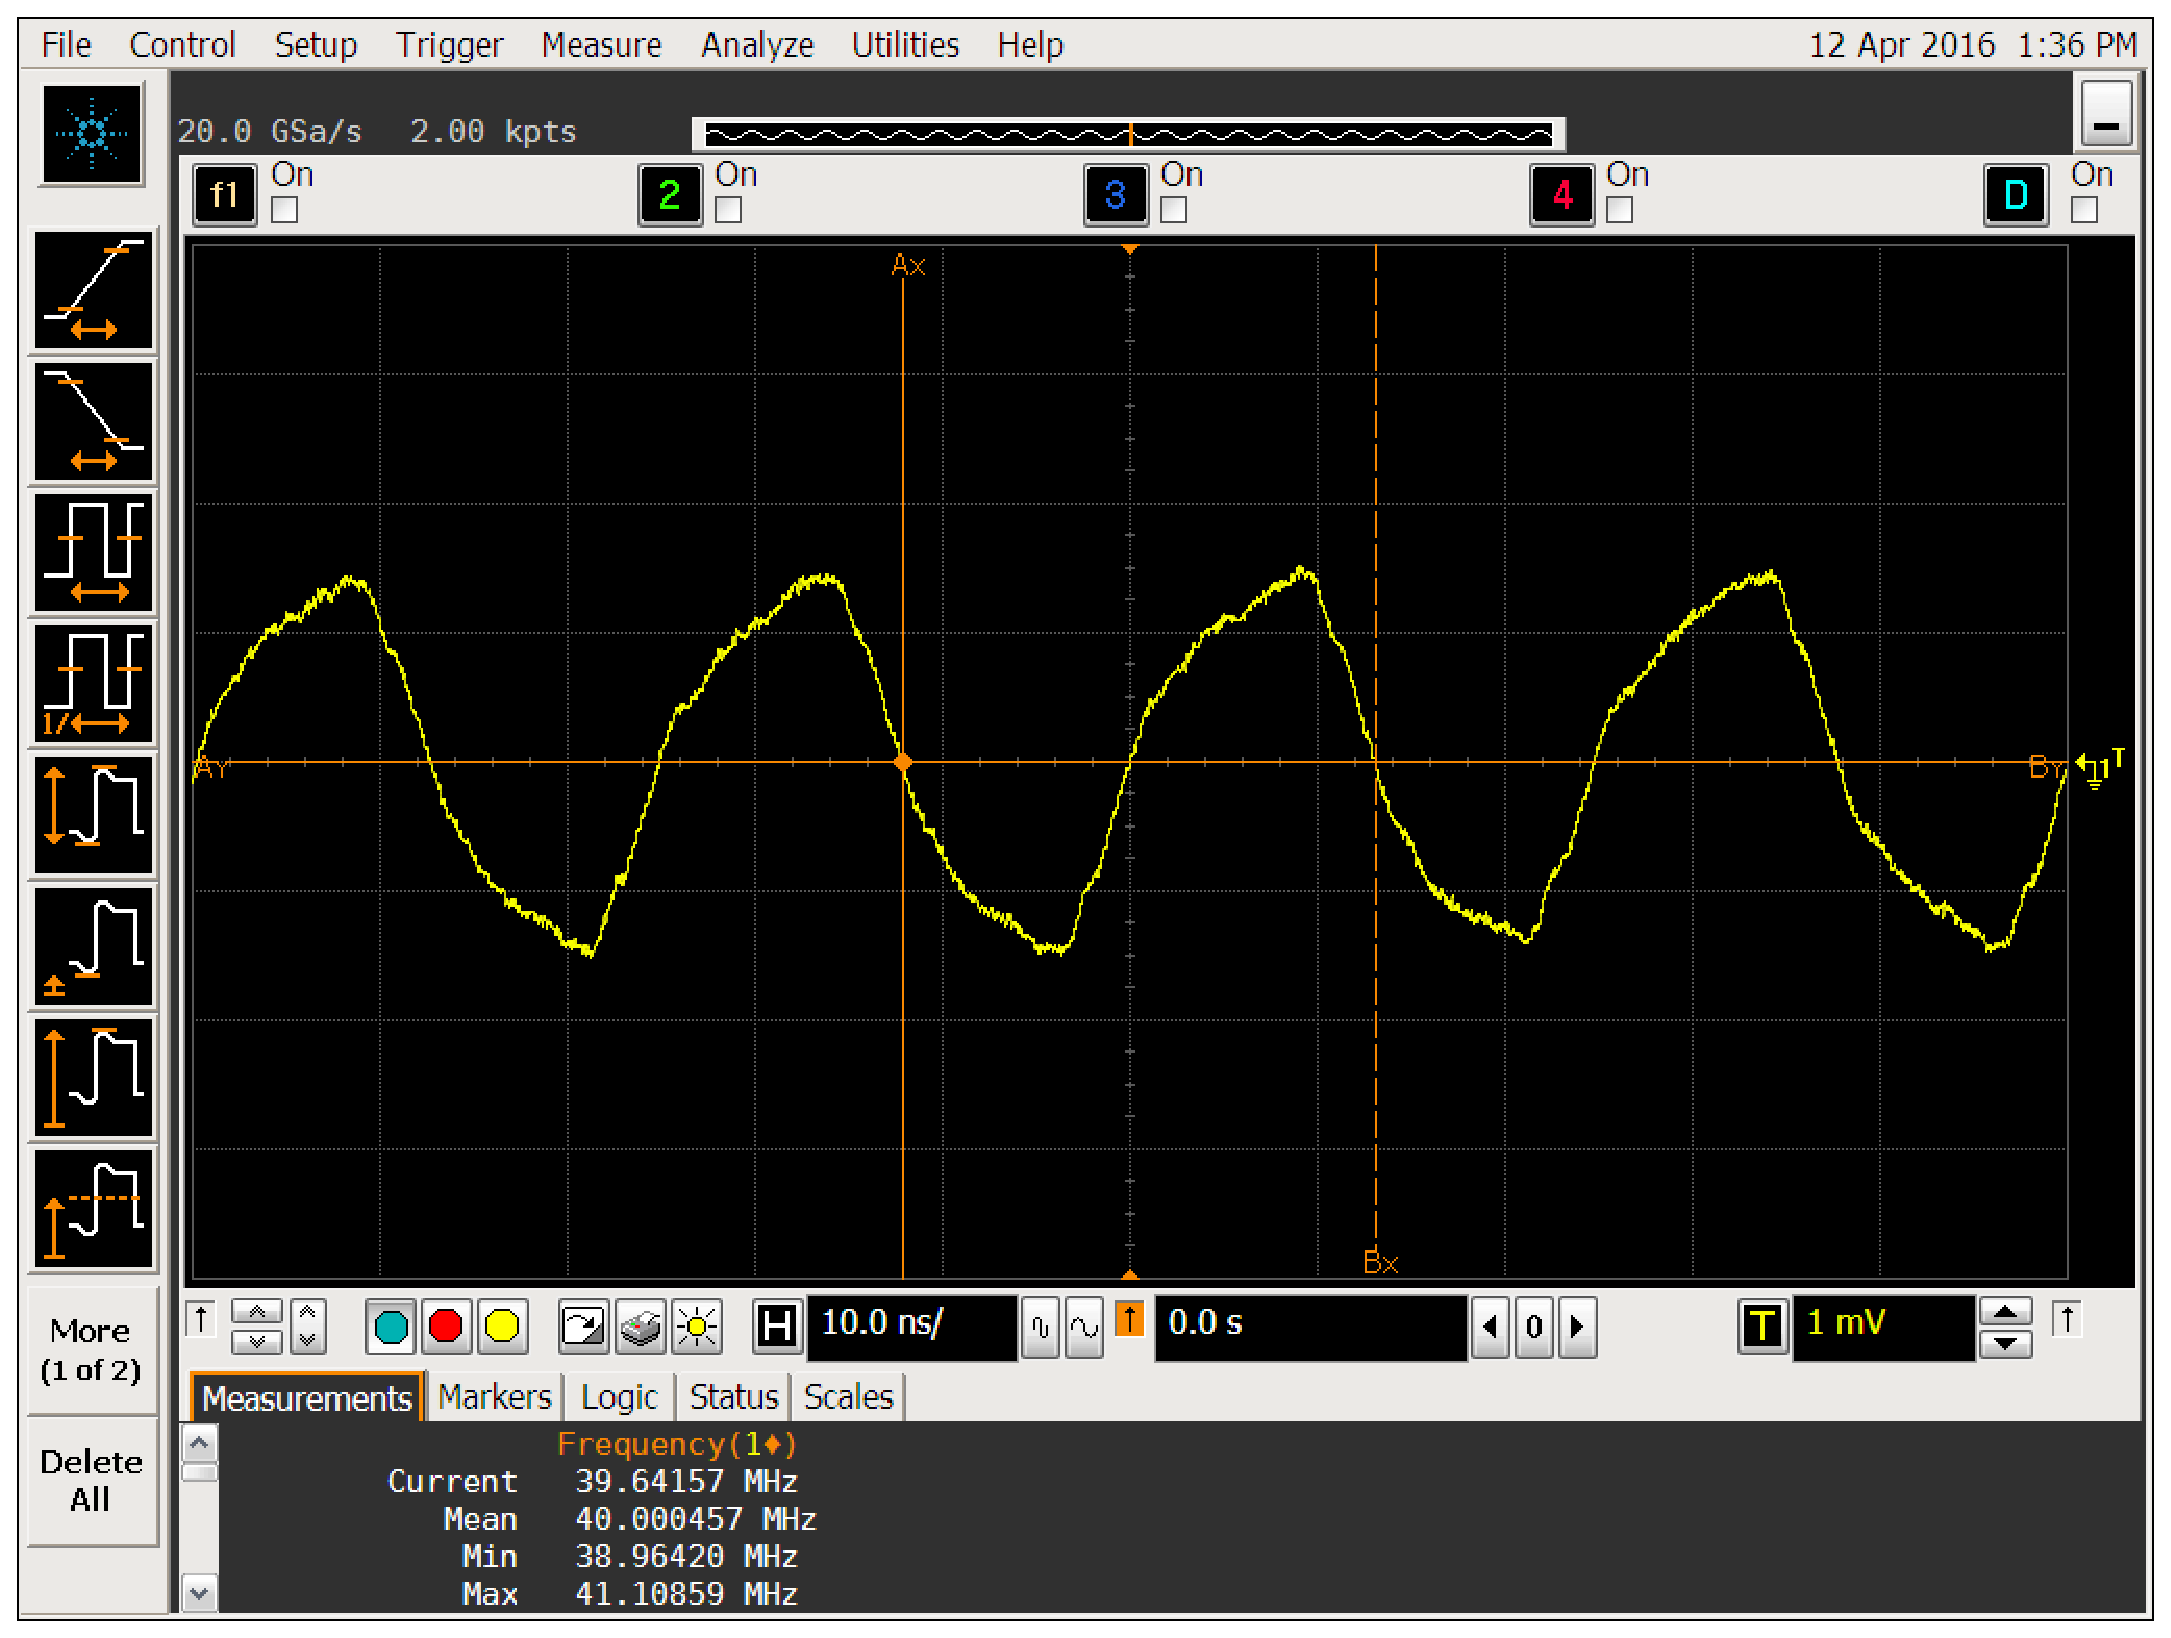
\includegraphics[width=0.85\textwidth]{./figures/oscill_ad9361_dac_clk}
    \caption{ DAC Clock Output
    \label{fig:dacclk}}
\end{figure}

\begin{figure}[htbp]
    \centering
    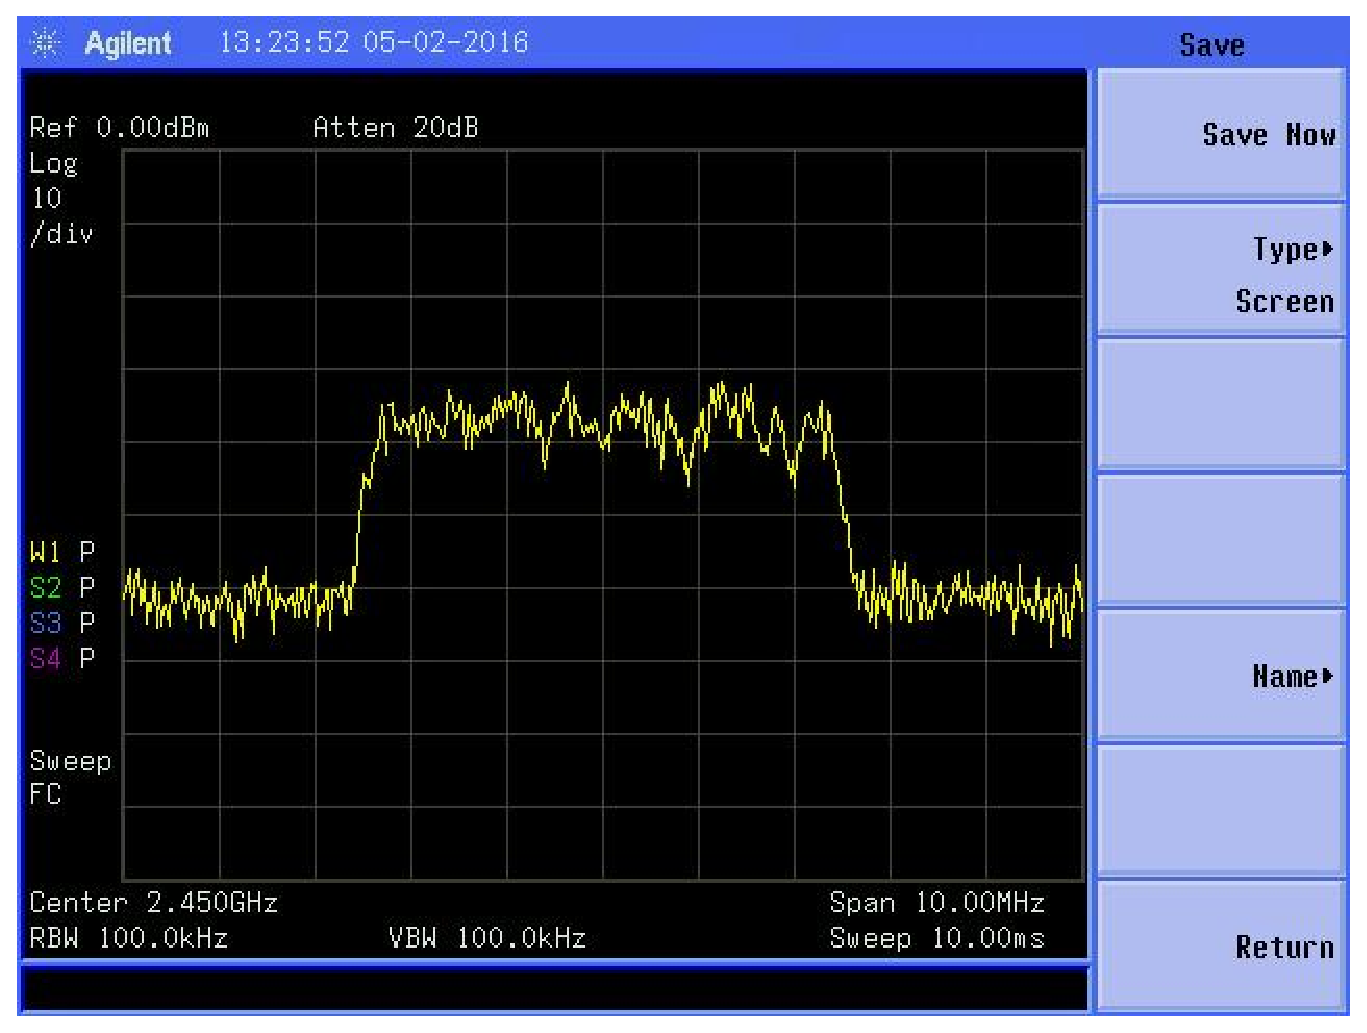
\includegraphics[width=0.85\textwidth]{./figures/lte_5m}
    \caption{ LTE signal output from FMComms2 Spectrum
    \label{fig:lte5m}}
\end{figure}

\vfill
\clearpage

\section{Reception Tests (ADC)}
\label{result:adc}

\begin{figure}[htbp]
    \centering
    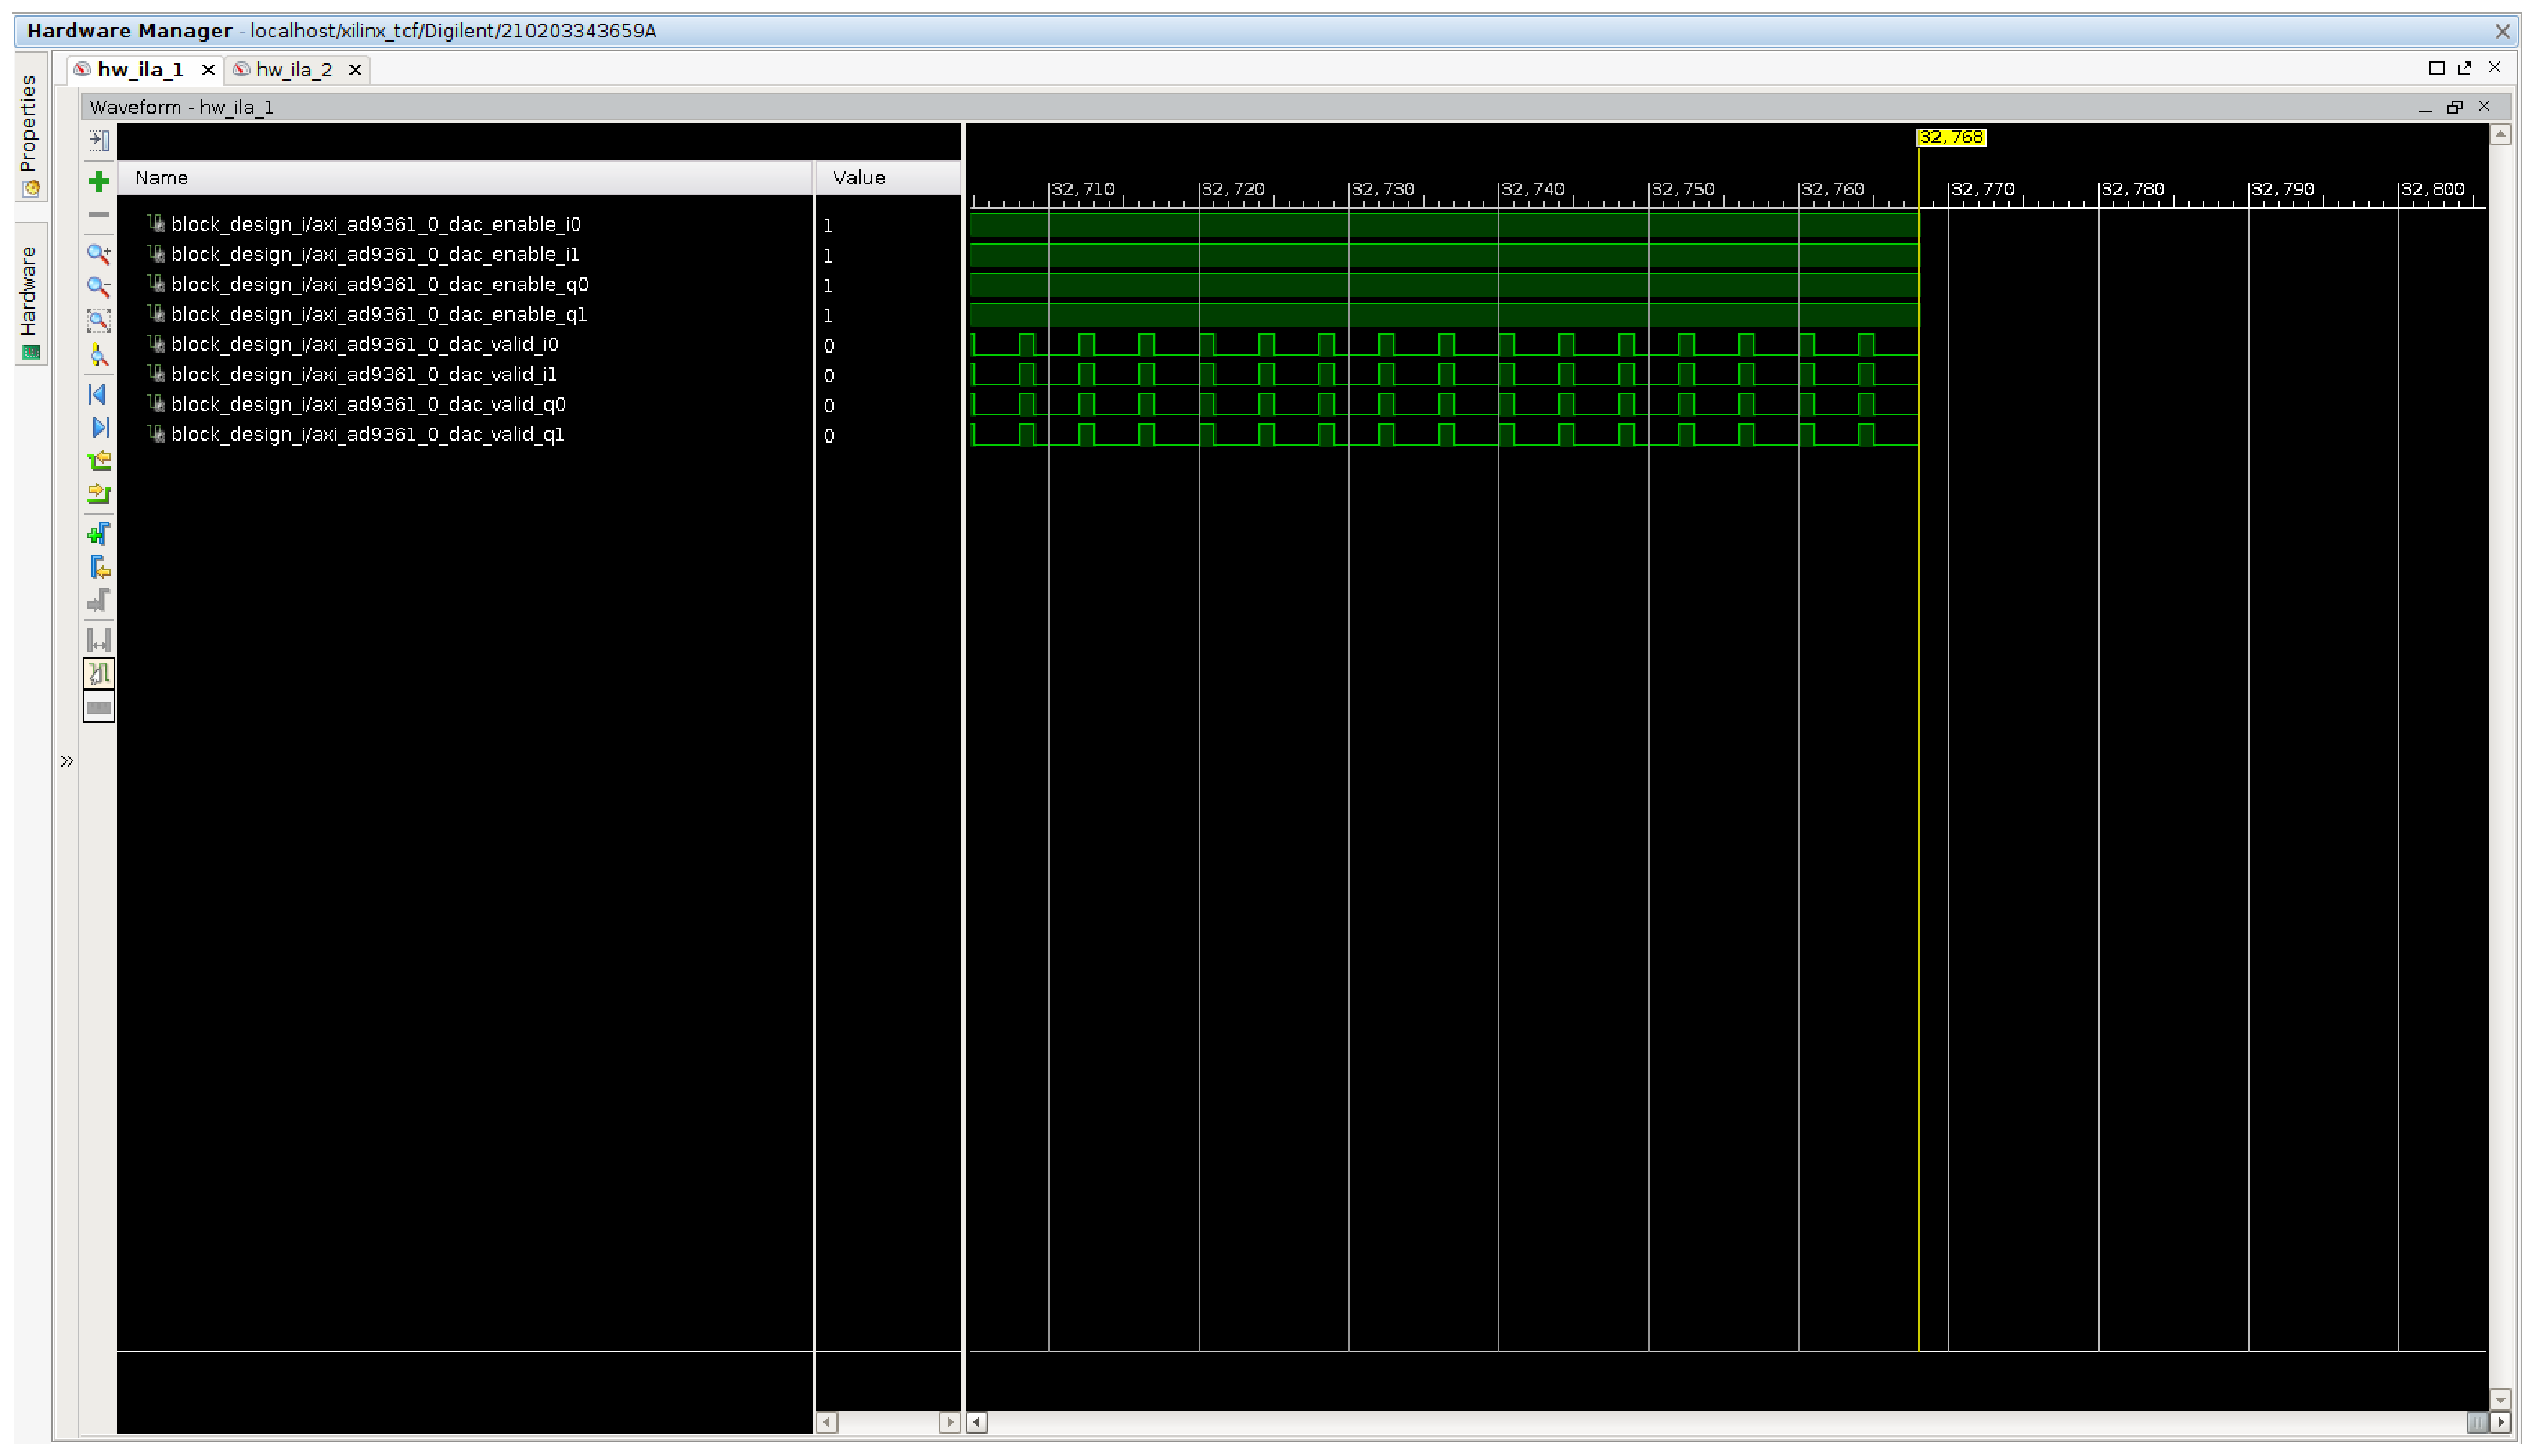
\includegraphics[width=0.85\textwidth]{./figures/dac_signals}
    \caption{ DAC signals controlling data writing
    \label{fig:adcsignals}}
\end{figure}

\vfill
\clearpage

\section{Optimum Results}
\label{result:optimum}

The expected transmission of lTE signals are below demonstrated by the Analog
Devices IIO scope application.

\begin{figure}[htbp]
    \centering
    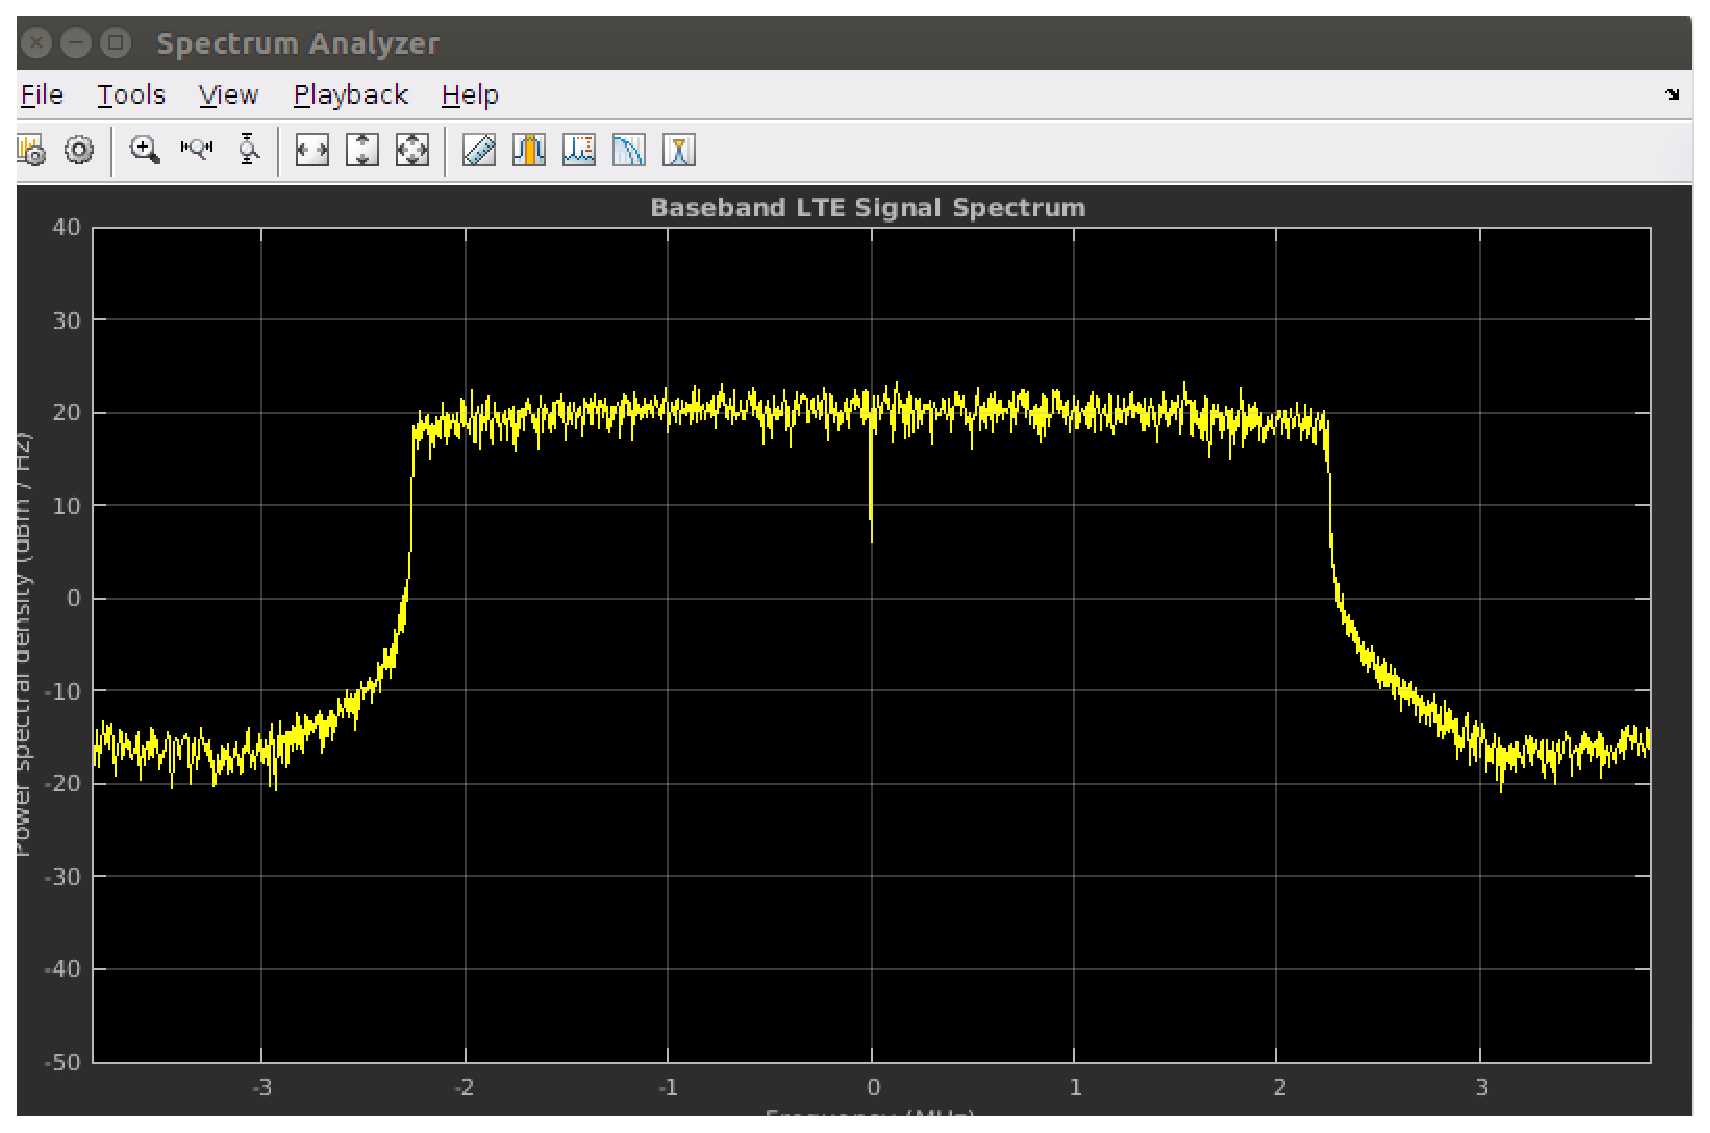
\includegraphics[width=0.65\textwidth]{./figures/lte_spectrum_iio}
    \caption{ LTE Spectrum
    \label{fig:ltespectrumiio}}
\end{figure}

\begin{figure}[htbp]
    \centering
    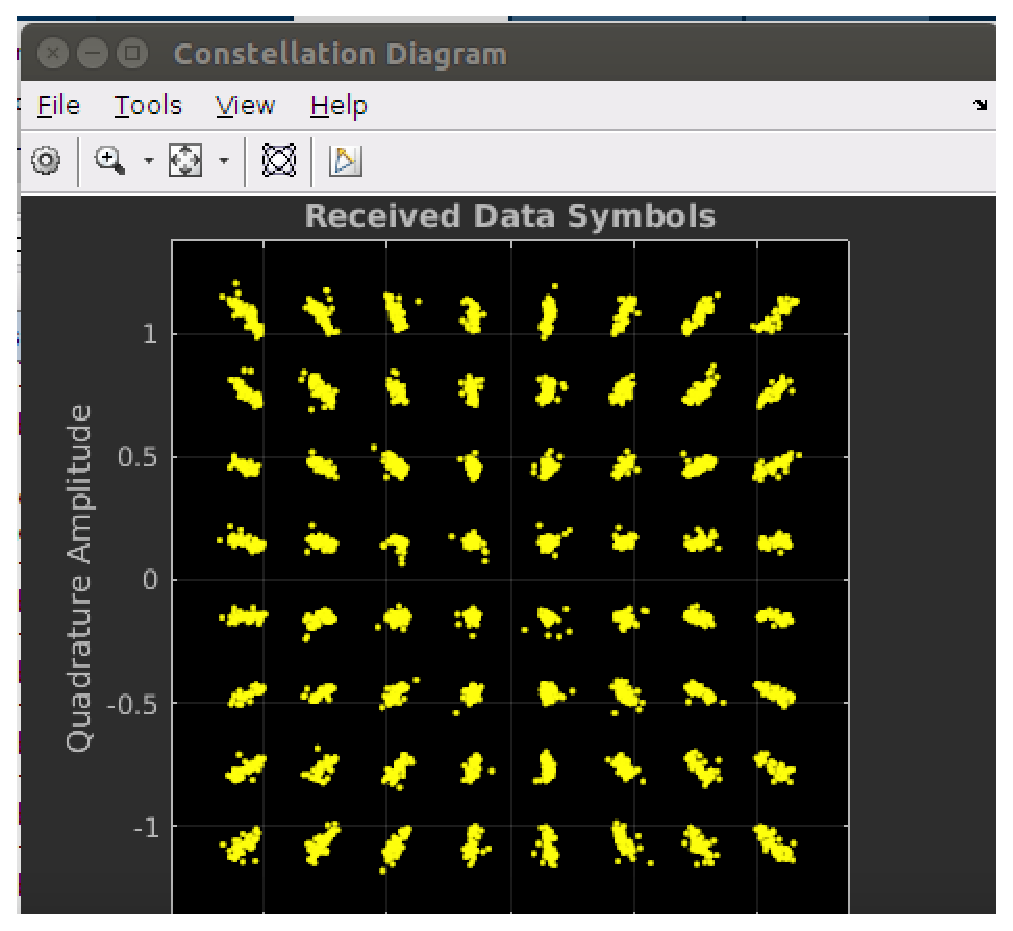
\includegraphics[width=0.65\textwidth]{./figures/lte_constellation_iio}
    \caption{ LTE Constellation
    \label{fig:lteconstellationiio}}
\end{figure}

\begin{figure}[htbp]
    \centering
    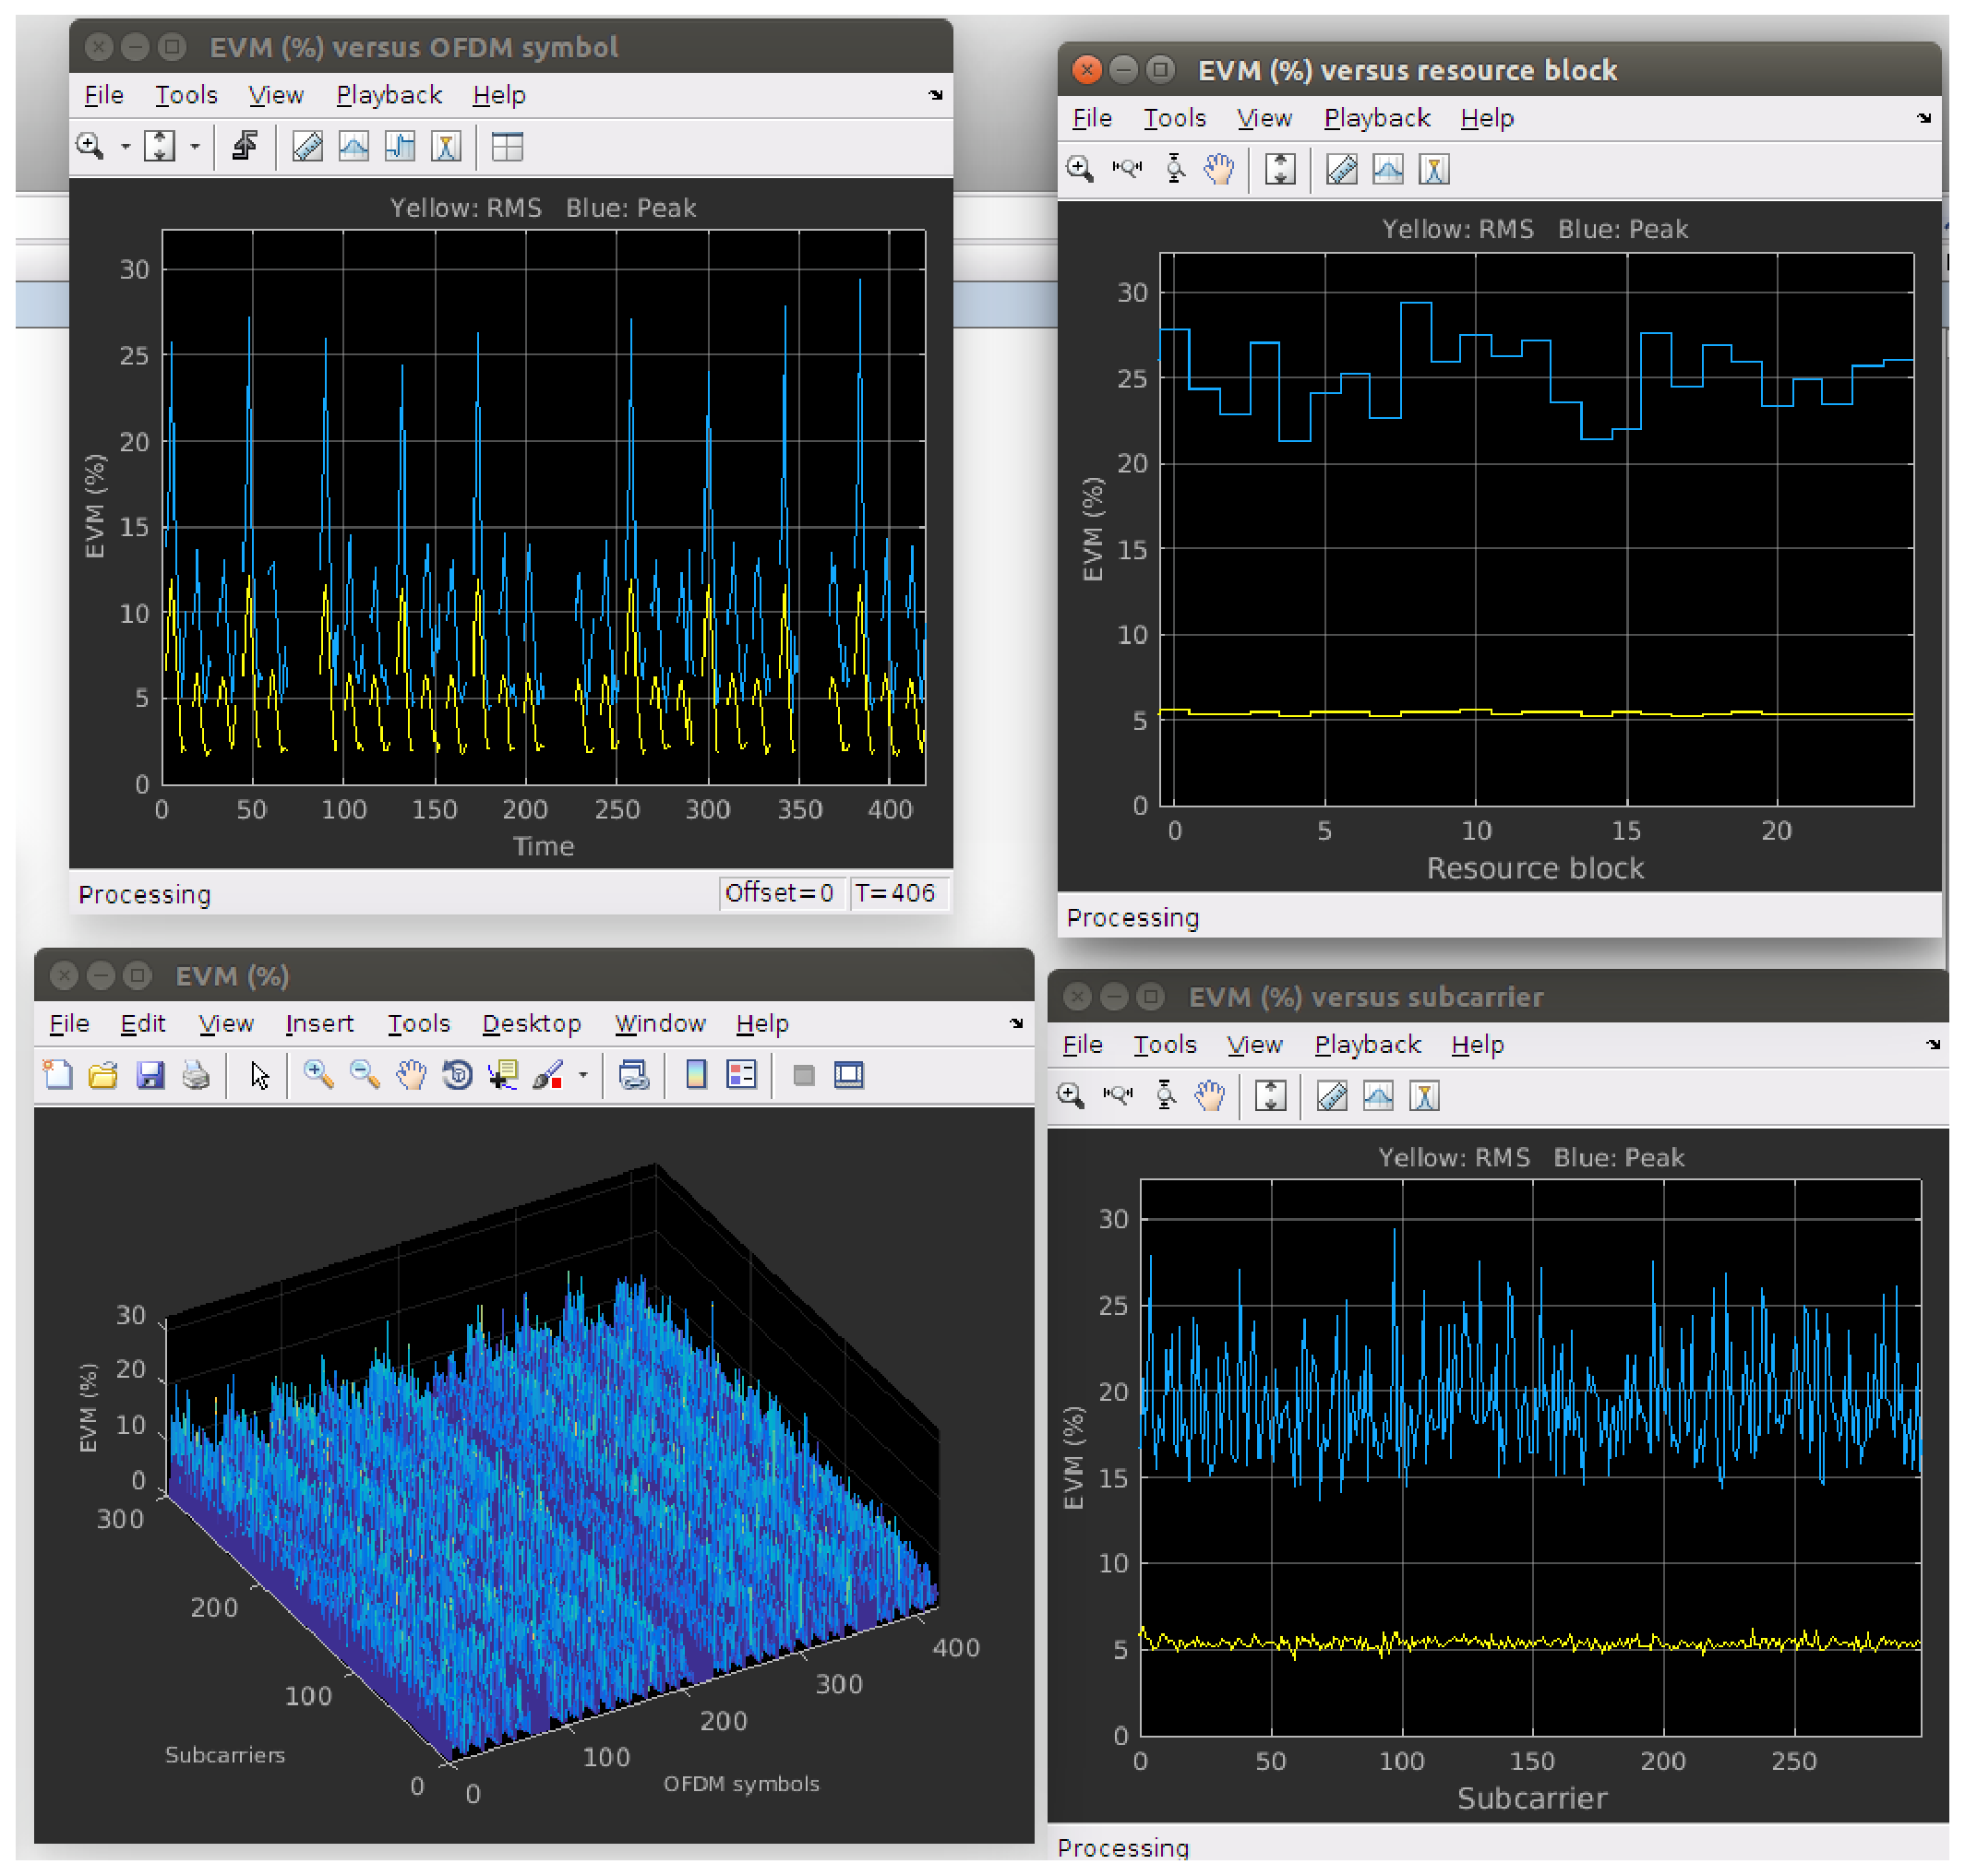
\includegraphics[width=0.85\textwidth]{./figures/lte_evm_iio}
    \caption{ LTE EVM
    \label{fig:lteevmiio}}
\end{figure}

\vfill
\clearpage
